\documentclass[11pt,a4paper]{article}

\usepackage[margin=2.5cm]{geometry}
\usepackage[utf8]{inputenc}
\usepackage{parskip}
\usepackage{todonotes}
\usepackage{microtype}
\usepackage{amssymb,amsmath}
\usepackage{mathpazo}
\usepackage{longtable,booktabs}
\usepackage{graphicx}

\usepackage{hyperref}
\usepackage[capitalise,noabbrev,nameinlink]{cleveref}
\hypersetup{
  pdftitle={Introduction to the design of the Data Diffusion and Networking for Cardano/Shelley},
  pdfborder={0 0 0},
  breaklinks=true
}

\begin{document}

\title{Introduction to the design of the
       Data Diffusion and Networking for
       Cardano/Shelley \\
       Part 1 (overview)\footnote{Supplemented by a Part 2 which is a
       Reference Document aimed at implementers of Shelly.
  \href{https://hydra.iohk.io/build/1011577/download/1/network.pdf}{{https://hydra.iohk.io/build/1011577/download/1/network.pdf}}} \\ \vspace{1cm}
       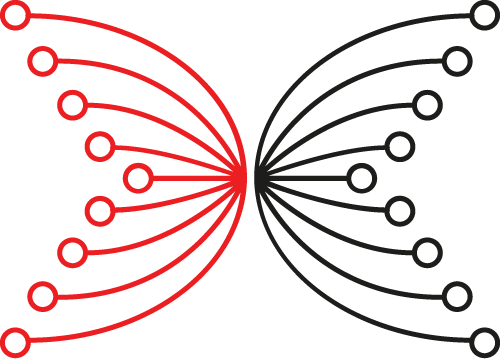
\includegraphics[width=1.95833in,height=1.40669in]{./media/image3.png}
  }
\date{}

\maketitle

\tableofcontents

\section{Revision History}
\label{revision-history}

\begin{longtable}[]{@{}llll@{}}
\toprule
\textbf{Version} & \textbf{Date} & \textbf{Change} &
\textbf{Reason}\tabularnewline
\midrule
\endhead
0.1 & 2020-05-21 & Created & Started from version 1.5 of internal
document.\tabularnewline
1.0 & 2020-05-28 & Revised & Edits to remove irrelevant and redundant
material\tabularnewline
1.1 & 2020-08-05 & Revised & Resolving remaining points and correcting
headings\tabularnewline
& & &\tabularnewline
& & &\tabularnewline
& & &\tabularnewline
& & &\tabularnewline
& & &\tabularnewline
& & &\tabularnewline
& & &\tabularnewline
& & &\tabularnewline
& & &\tabularnewline
& & &\tabularnewline
& & &\tabularnewline
& & &\tabularnewline
\bottomrule
\end{longtable}

\section{Executive Summary}
\label{executive-summary}

\emph{\textbf{Purpose of document.} }

We explain the technical requirements and key constraints for the
networking layer of the Cardano Shelley implementation of Ouroboros
Praos. The key functional role of this layer is the data diffusion of
blocks, transactions and(and other information to be shared) in Cardano
Shelly. The general design was created to meet the likely needs of
highly distributed, publicly facing PoS blockchain system in general.

The technical requirements are expressed in terms of the key business
requirements provided at the project's outset then refined with the IOHK
business team.

We give design requirements, compare with existing protocols, and
describe the rationale for the solution adopted by the IOHK Networking
Team.

\emph{\textbf{Who the original was for:. }}

\todo[inline]{ND: Need Biz Level decision - is this still the avowed intended audience?}

It was intended to provide a management-level overview of the Cardano
Shelley networking layer to inform strategic decision making and to
provide confidence in the proposed networking implementation,
supplementing this with a detailed technical analysis explaining the
design and implementation to the Engineering and Quality Assurance team.

\emph{\textbf{Where does it fit in the overall documentation scheme
(dependencies, technical/management etc)?}}

We build and expand on the design requirements from the Ouroboros Praos
paper. It links with the Shelley Ledger specification.

The networking solution is being deployed as part of the Shelley
\emph{mainnet} implementation, linking with the \emph{ledger, wallet}
and other implementations. Design decisions will also be used to inform
the future \emph{testnet} implementations, as appropriate to ensure the
necessary rapid deployment. The document will be used to derive
information for subsequent testing and deployment.

\emph{\textbf{Achievements and Status. }}

The business requirements necessitated a bespoke protocol design,
compatible with hard real-time concerns, security concerns, and a
globally distributed network. This is a novel, technically complex
issue. The resulting implementation is carefully designed but relatively
simple. It has been validated, substantially implemented and tested.

\section{Technical Summary and Motivation for the New Design}
\label{technical-summary-and-motivation-for-the-new-design}

The networking requirements for a Proof-of-Stake (PoS) system, such as
Ouroboros, differ from those of a Proof-of-Work (PoW) system, such as
Bitcoin or Ethereum.

In PoW, adversaries must expend hashing power, which honest players can
check in a cheap and stateless way. Honest nodes in a PoS system lack
this advantage, which tips the balance towards the attacker, so it is
necessary to mitigate this with careful design. Notably, off-the-shelf
overlay network solutions tend not to consider such attacks. Existing
solutions have been assessed, but the cost of retrofitting them to
address the new balance of power between the adversary and honest
players above is easy to underestimate and they would require
substantial modification which would negate any advantages of code
reuse. This is a major reason we undertook a from-scratch development.

Our design is simple and modular and interleaves the three parts of the
Ouroboros distributed consensus algorithm: chain transmission,
validation and selection. The design uses a stateful chain
synchronisation protocol\footnote{We follow a stream processing paradigm
  adapted for the eventual finality behaviour of blockchain systems.},
both for the node-to-node case and for the case of local IPC with
wallets/explorers etc. The design is extensible for future flexibility,
and has a plug-in consensus algorithm to support the anticipated
evolution of Ouroboros. It includes a network protocol framework that
currently is used for three application-level protocols. Protocols can
be added or changed for future requirements. Protocols can be pipelined
to enable effective use of network resources (all the node-to-node
protocols are fully pipelined), and have been designed for
decentralisation. The framework is reused for local client IPC, such as
the explorer backend.

The implementation has been kept simple to minimise complexity and
attack surface. It is fully integrated with the rest of the node and is
working in the Shelly mainnet. At the time of writing only one component
has not yet been deployed, namely the peer selection and subscription
management (outline design in \cref{decentralisation-design}
\cref{decentralisation-design}).

\section{Introduction}
\label{introduction}

A blockchain is a mechanism for computing \emph{distributed consensus}
on a global scale, i.e. coming to global agreement on a sequence of
events, in the presence of `bad actors' trying to bias or disrupt the
system, and without a centralised authority.

Distributed consensus algorithms fall into two main camps: proof-of-work
(PoW) and proof-of-stake (PoS).

\begin{itemize}
\item
  \begin{quote}
  \textbf{Proof-of-work} algorithms, like Bitcoin's, are a race to
  `mine' blocks. The winner gets to add a block on the blockchain, and
  collects rewards for doing so.\\
  Miners consume vast computational resources as they compete on a
  global scale.
  \end{quote}
\item
  \begin{quote}
  \textbf{Proof-of-stake} algorithms take turns to produce blocks in
  proportions that are determined by the users' stakes in the system.\\
  Blocks can be produced efficiently and frequently, improving
  throughput and settling time\footnote{The amount of time that must
    pass for the consensus to be considered immutable.}, but at the risk
  of creating forks if a previous block fails to reach the next block
  producer in time.
  \end{quote}
\end{itemize}

Cardano is a third-generation blockchain\footnote{Bitcoin was the first
  generation. Ethereum is an example of a second generation blockchain.}
based on a new proof-of-stake consensus algorithm called Ouroboros
{[}BGKR17, BGKRZ19{]}. Cardano's first implementation,
\href{https://cardanoroadmap.com/en/byron/}{{Byron}}, was introduced in
September 2017.

Shelley is a full, modular, reimplementation of Cardano, organised into
two main functional components:

\begin{enumerate}
\def\labelenumi{\arabic{enumi}.}
\item
  \begin{quote}
  the \emph{data diffusion} layer, which governs how data propagates
  between Cardano nodes, and
  \end{quote}
\item
  \begin{quote}
  the \emph{consensus} layer, which implements the Ouroboros algorithm
  and applies the ledger rules.
  \end{quote}
\end{enumerate}

Cardano is a distributed algorithm. Consequently in the Shelley
implementation each network node runs a Shelley \emph{instance}, whose
functions interact via the data diffusion component.

This document describes, for the Shelley implementation of Cardano:

\begin{enumerate}
\def\labelenumi{\arabic{enumi}.}
\item
  \begin{quote}
  the goals and constraints of the data diffusion component,
  \end{quote}
\item
  \begin{quote}
  the design decisions that were made in meeting these goals and
  constraints, and
  \end{quote}
\item
  \begin{quote}
  why those particular decisions were made.
  \end{quote}
\end{enumerate}

A note on terminology: while ``data diffusion'' and ``network'' mean
slightly different things -- technically, data diffuses \emph{across} a
network -- for simplicity we may use these terms synonymously in this
document.

\subsection{Structure of the document}
\label{structure-of-the-document}

\todo[inline]{ND: May be missing "this is how the bits fit together" part of the story - this could be as diagram(s) or text.
The aim would be to "tell them what we are going to tell them" to provide some hooks for the reader to attach ideas to as they are presented.}

This document is structured as follows:

\begin{enumerate}
\def\labelenumi{\arabic{enumi}.}
\item
  \begin{quote}
  In \cref{overview} we describe the overall
  implementation of the Ouroboros algorithm, and summarise the key
  constraints and design decisions, in particular how validation and
  forwarding have to be interleaved in order to deliver a robust
  implementation.
  \end{quote}
\item
  \begin{quote}
  In \cref{distributed-consensus-on-a-global-scale} we discuss how the
  constraints of the physical world impact on a distributed ledger
  system and also the implications of running an autonomous
  collaborative algorithm with hard real-time constraints on a
  global-scale. We consider the threats that such a system faces because
  it is global and open, including the possibility of \emph{adversarial
  nodes} within the system and the vulnerability of being on the global
  Internet, such as exposure to DDoS attacks.
  \end{quote}
\item
  \begin{quote}
  In \cref{analysis-of-alternative-approaches} we consider a range of
  published approaches to transferring information between nodes and the
  extent to which they are able to meet the constraints and deal with
  the threats that were discussed in
  \cref{distributed-consensus-on-a-global-scale}.
  \end{quote}
\item
  \begin{quote}
  In \cref{operational-environment-and-constraints} we enumerate the
  operational environment and the constraints that are derived from the
  business requirements from \cref{business-requirements}.
  \end{quote}
\item
  \begin{quote}
  In \cref{key-design-decisions} we discuss our development
  approach and design decisions.
  \end{quote}
\item
  \begin{quote}
  In \cref{outstanding-unresolved-issues} we look at currently
  unresolved issues.
  \end{quote}
\item
  \begin{quote}
  In the appendix we provide: the previously-agreed business
  requirements (\cref{business-requirements}); numerical models of TCP
  performance (\cref{tcp-rpc-response-behavior}), the network scaling
  (\cref{model-of-network-scaling}), and the leadership distribution in
  Ouroboros Praos (\cref{performance-model-of-ouroboros-praos}); and
  give a detailed description of the software components that are
  required by our solution (\cref{ouroboros-network-components}).
  \end{quote}
\end{enumerate}

\section{Overview}
\label{overview}

This document concerns the requirements, constraints and design
decisions of the network layer of Cardano. However, the network layer
design is fundamentally shaped by

\begin{itemize}
\item
  \begin{quote}
  the constraints and design of the Cardano consensus layer, and
  \end{quote}
\item
  \begin{quote}
  keeping extensibility in mind for the product roadmap.
  \end{quote}
\end{itemize}

Thus far, the network parts exist almost exclusively to serve the needs
of the consensus implementation\footnote{Although they have been written
  in a modular way to facilitate extension and re-use.}. So to
understand the design constraints and design decisions for the network
layer implementation we must first consider the requirements,
constraints and design decisions of the consensus layer implementation.

\subsection{Consensus constraints and design decisions}
\label{consensus-constraints-and-design-decisions}

Cardano as a cryptocurrency system fundamentally relies on an
implementation of Ouroboros {[}BGKR17, BGKRZ19{]}. The underlying
properties of Ouroboros\footnote{Specifically, liveness and persistence
  -- see below.} ensure, \emph{by design,} that Cardano users can submit
valid transactions and can rely on them being incorporated into the
\emph{immutable} prefix of the cryptocurrency ledger. This is despite
the system being open (accessible to those with minimal or no stake)
where adversaries may attempt to steal money or cripple the system, and
operating over the public Internet where the network load, bandwidth and
latency may be highly variable and unpredictable.

It follows that a key part of the commercial offering is that Cardano,
being based on an implementation of Ouroboros, can actually achieve
these goals and so provide a sound underpinning of the cryptocurrency,
while operating on the public internet network with a public IP and thus
fully exposed to bad actors.

The key requirements for the Ouroboros implementation come from the
Ouroboros specification as embodied in the published and peer-reviewed
\href{https://iohk.io/research/papers/}{{papers}}, and from business
requirements (see \cref{business-requirements})
including quantitative non-functional requirements.

There are three levels of refinement:

\begin{enumerate}
\def\labelenumi{\arabic{enumi}.}
\item
  \begin{quote}
  The underpinning academic papers (e.g. {[}BGKR17, BGKRZ19{]}) that
  give a \emph{mathematical description} of the algorithm;
  \end{quote}
\item
  \begin{quote}
  An \emph{implementation design} that:
  \end{quote}

  \begin{enumerate}
  \def\labelenumii{\alph{enumii}.}
  \item
    \begin{quote}
    Can be shown equivalent to the mathematical description (informally
    at first, formal proof to follow as and when time permits);
    \end{quote}
  \item
    \begin{quote}
    Can be implemented in a real-world distributed computational
    setting;
    \end{quote}
  \item
    \begin{quote}
    Does not introduce new possibilities -- with respect to the
    mathematical description -- for attackers to disrupt or subvert the
    system, or at least includes mitigations for any vulnerabilities
    that it does introduce;
    \end{quote}
  \end{enumerate}
\item
  \begin{quote}
  A \emph{software implementation} that follows from the implementation
  design;
  \end{quote}

  \begin{enumerate}
  \def\labelenumii{\alph{enumii}.}
  \setcounter{enumii}{3}
  \item
    \begin{quote}
    The correspondence between the two being checked through tests,
    property checking etc.;
    \end{quote}
  \item
    \begin{quote}
    That is efficient, modular and easy to maintain; and
    \end{quote}
  \item
    \begin{quote}
    That does not introduce any further possibilities -- with respect to
    the implementation design -- for attackers to disrupt or subvert the
    system through refinements of or changes to the design, or at least
    includes mitigations for any that it does introduce.
    \end{quote}
  \end{enumerate}
\end{enumerate}

This section focuses on the first refinement step, from the mathematical
description to the implementation design.

The mathematical description of the Ouroboros algorithm is not intended
to be a directly implementable design. For example, transmitting entire
blockchains is impractical, but is a valid specification of an outcome
to be achieved by a practical design. Substantial work was required to
refine the mathematical description to an implementation design.

Ouroboros establishes strong properties of \emph{progress} (liveness)
and \emph{persistence}\footnote{These two properties are the
  underpinning of the Cardano cryptocurrency ledger.} , based on
surprisingly weak assumptions {[}BGKRZ19, Section 1{]}, and in an
environment with potentially powerful adversaries. This environment
combined with the capabilities of the adversaries collectively comprise
the threat model (see \cref{high-level-threat-model}).

\subsubsection{Interleaving transmission and validation}
\label{interleaving-transmission-and-validation}

\paragraph{The Ouroboros specification}
\label{the-ouroboros-specification}

Ouroboros \emph{as an algorithm specification} is elegantly modular,
comprising:

\begin{enumerate}
\def\labelenumi{\arabic{enumi}.}
\item
  \begin{quote}
  Reliable chain broadcast; followed by
  \end{quote}
\item
  \begin{quote}
  Chain validation; followed by
  \end{quote}
\item
  \begin{quote}
  Chain selection
  \end{quote}
\end{enumerate}

All current members of the Ouroboros family have this same structure,
which suggests using a parameterized consensus design that can be
instantiated for BFT, Praos and the other variants\footnote{The new
  Byron-compatible consensus algorithm is Ouroboros ``Permissive'' BFT,
  a custom variation designed to handle the transition from Ouroboros
  Classic to Ouroboros BFT. The Shelley consensus algorithm is the
  sequential composition of Ouroboros Permissive BFT followed by the
  combination of Ouroboros Praos with a transitional BFT overlay
  schedule.} that are used in Cardano Byron and Cardano Shelley.

In the specification, the reliable chain broadcast is expected to
achieve delivery within fixed deadlines. In practice this is, of course,
impossible: delivery with high probability is the best that can be
achieved. Failure to meet deadlines in the \emph{typical} case or for an
extended period of time is fatal to the system, but occasional failure
simply eats into the ``adversarial stake budget''. IOHK's Ouroboros
researchers have set a practical target of achieving the deadline in
95\% of cases.

A simple broadcast implementation is impractical because adversarial
players can use it to DoS the system with invalid chains. By
deliberately over-using the broadcast mechanism, adversarial players can
consume the system's limited broadcast capacity to the point where
chains sent by honest players \emph{consistently} fail to reach the next
slot leader within the required deadline.

It is also impossible to make a \emph{simple} alteration to a broadcast
algorithm to filter out bad data sent by adversarial players: A simple
alteration to a broadcast algorithm would require a \emph{stateless}
validation check. However, no known practical\footnote{There is of
  course an \emph{impractical} stateless check, which is to validate the
  entire broadcast chain from the Genesis.} stateless check can exclude
invalid chains for Ouroboros. The validation check for Ouroboros relies
on having a full and (nearly) up-to-date ledger state. Having a full
ledger state depends on the other two pieces of Ouroboros functionality,
the chain validation and chain selection. Thus, to validate new
chains/blocks, we are required to run \emph{all} of the consensus
implementation. We cannot, therefore, use a straightforward modification
of a broadcast algorithm.

Therefore, existing off-the-shelf implementations of the broadcasting
paradigm (\emph{pure} \emph{gossip} and/or \emph{pub/sub}) are hard to
reuse; any form of broadcast in a PoS context opens up trivial DoS attacks, in
which the asymmetric power of broadcast is weighted in favour of the
attacker. Mitigating that problem is impossible in practice, since every
end user would be susceptible to attack. At best we can use broadcast as
an inspiration for the overall consensus design.

As if validation was not challenging enough, broadcast can also be used
by adversaries who become (or have recently become) slot leader in order
to send an unbounded number of \emph{valid} chains. Avoiding this
requires the Ouroboros chain selection and chain validation features,
which can be used to reduce the number of chains broadcast to within a
plausible bound that could fit within the available resources.

\paragraph{Consequences of PoS vs PoW}

A crucial difference exists between PoS and PoW at the network layer,
with significant design consequences: in PoW-based systems,
proof-of-work itself gives honest nodes an advantage over adversarial
nodes (as listed below), and this enables system designs that are
simpler and more modular. There is no such advantage for honest nodes in
PoS-based systems such as Ouroboros.

In PoW systems:

\begin{itemize}
\item
  \begin{quote}
  The number of different block headers with a valid PoW that can be
  constructed (over any given period of time) is bounded by the total
  available hashing power in the world. In Bitcoin for example this is
  one header every ten minutes on average.
  \end{quote}
\item
  \begin{quote}
  The header PoW can be checked with little computational cost. This
  does not require any significant or recent state, only a
  vaguely-recent lower bound on the hashing difficulty value is needed.
  \end{quote}
\item
  \begin{quote}
  Such a cheap and simple test can be easily integrated into existing
  distributed algorithms such as broadcast algorithms.
  \end{quote}
\end{itemize}

By contrast, with PoS in Ouroboros:

\begin{itemize}
\item
  \begin{quote}
  There is no equivalent of the PoW check that is expensive for the
  adversaries and cheap for the honest nodes: adversaries can create
  many apparently valid or actually valid candidate headers or whole
  chains.
  \end{quote}
\item
  \begin{quote}
  Block headers can only be fully validated with access to a very recent
  copy of the full ledger state, and the other preceding headers --
  which is not a simple stateless check.
  \end{quote}
\item
  \begin{quote}
  Having the full ledger state relies on the other two pieces of
  Ouroboros functionality: chain validation and chain selection.
  \end{quote}
\end{itemize}

Thus we conclude that the Ouroboros broadcast functionality cannot be
implemented in isolation, and that an integrated design is required that
combines all three areas of Ouroboros functionality: chain broadcast,
validation and selection.

\paragraph{Bounding the resource use of honest nodes}

An important consideration in making a more detailed design for
Ouroboros stems from the nature of the proof of the Ouroboros
properties: the proof can be thought of as starting with

\emph{``For all possible actions of the adversaries \ldots{}'' }

s we refine our design by making more detailed and realistic the
mechanisms by which (honest and adversarial) nodes interact, so we also
expand the threat model, because the more detailed design gives
adversaries more ways to interact with the honest nodes.

For example, a single abstract broadcast interaction may be replaced by
a collection of RPC interactions running atop layers of lower level
protocols, each with their own complex interactions. We discussed in
\cref{the-ouroboros-specification} the
problems that arise when the resource use of honest nodes is under the
control of adversaries; this too can only get worse during design
refinement or implementation, as we provide new mechanisms to interact.

Thus, a fundamental constraint when evaluating consensus designs is to
find one with a plausible argument for bounding the resource use of
honest nodes, given \emph{all} the possible actions of the adversary
that are enabled by the design -- otherwise, the security guarantees of
the mathematical consensus algorithm are negated. This is a high bar --
even with the caveats of ``plausible'' and ``informal''. The contrasts
with the orthodox approach, which only solves the simpler problem of
solving or mitigating against known classes of attack\footnote{For
  example, much of the critique of Kademlia (ours in
  \cref{kademlia} and others' {[}MHG18{]})
  comes down to the fact that it followed the orthadox design approach.
  It does not start with a threat model and establish positive results.
  Many academic papers on Kademlia establish negative results: they find
  flaws and then fix or mitigate them. We must however suspect that
  there are more flaws to be found, because none establish a positive
  result.}.

After much effort evaluating various designs that incorporated some
aspect of broadcast (e.g. broadcast of block headers), we were unable to
find a design for which we could make even an informal resource bounds
argument. The designs we studied also tended to be excessively complex.

In abandoning the notion of broadcast we move from a situation in which
a participating node receives information from \emph{all} other nodes to
one in which it receives information from only \emph{some} of the other
nodes, which we refer to as its `peers'. Nodes are then connected in a
graph through which information flows.

Our final design thus interleaves (in a sense made more precise below)
the three parts of the Ouroboros algorithm functionality:

\begin{itemize}
\item
  \begin{quote}
  chain transmission,
  \end{quote}
\item
  \begin{quote}
  chain validation and
  \end{quote}
\item
  \begin{quote}
  chain selection.
  \end{quote}
\end{itemize}

These three parts are used at every node in the graph that indirectly
connects all (or at least most) nodes. This design turns out to be
relatively simple and could plausibly be refined further to (at least
informally) establish resource bounds.

Our design interleaves Ouroboros functionality in the following sense:
along any path through the graph of nodes, there will be multiple rounds
of chain transmission, validation and selection, with one round per hop
in the path. After the first design refinement\footnote{This design is
  an intermediate design refinement. Like the high level Ouroboros
  algorithm, it still uses elements that are not directly implementable
  (like transmitting whole chains). Further refinements will attain
  directly implementable design. This refinement process is a standard
  technique for modular design, allowing design options to be considered
  in relative isolation. This modularity is especially helpful if and
  when we apply formal methods to prove correctness of low level designs
  with respect to high level specifications.} step, our high level
algorithm is as follows:

\begin{itemize}
\item
  \begin{quote}
  each node transmits its current chain to its immediate neighbours;
  \end{quote}
\item
  \begin{quote}
  each node validates the incoming chain from each neighbour;
  \end{quote}
\item
  \begin{quote}
  each node does chain selection on the candidate chains;
  \end{quote}
\item
  \begin{quote}
  the selected chain becomes the node's new current chain, ready to be
  transmitted to its neighbours again; and
  \end{quote}
\item
  \begin{quote}
  when a node is a slot leader, it extends its own current chain with
  the new block.
  \end{quote}
\end{itemize}

By contrast, recall that in the original mathematical description of the
algorithm, the chains are broadcast to \emph{all} nodes, and \emph{then}
each node locally performs chain validation and selection over all the
chains that it receives.

It is worth noting again that this design is not `broadcast' in the
classical sense, and hence, as discussed earlier in
\cref{the-ouroboros-specification},
existing broadcast implementations (including multicast and pub/sub)
cannot easily be adapted to provide an implementation of this design. It
is nevertheless a relatively simple design and can be implemented
directly, with some further essential refinement.

\subsubsection{Block/body splitting}
\label{blockbody-splitting}

An essential and uncontroversial design refinement in any blockchain
implementation is to separate block headers and block bodies:

\begin{itemize}
\item
  \begin{quote}
  If blocks can be almost fully validated in O(1) time based on looking
  at only a small fixed size block header, then honest nodes can
  validate candidate chains with a small bounded amount of work.
  \end{quote}
\item
  \begin{quote}
  It also enables a design where a node can see blocks available from
  many immediate peers but can choose to download each block body of
  interest just once (from a peer of its choosing from which it is
  available). This saves network bandwidth\footnote{We also exploit this
    to choose a peer that we have reason to believe will deliver the
    block soonest.}.
  \end{quote}
\end{itemize}

In the case of Ouroboros, we can pack all the cryptographic consensus
evidence into the block header, leaving the block body containing only
the ledger data, and check that the block has been signed by a node that
is the slot leader. If we validate this in the context of a chain of
headers\footnote{We also need the ledger state, and there are some other
  technical constraints.}, then we can establish this is a plausible
candidate chain, thus we eliminate several potential resource draining
attacks.

So the design at this stage involves transmitting chains of headers
rather than whole blocks, and using a secondary mechanism to download
block bodies of interest\footnote{Blocks can be fetched from any peer
  who announces it, or from multiple sources if desired.}.

\subsubsection{Stateful chain-following}
\label{stateful-chain-following}

The next design decision revolves around how to implement the
transmission of chains of headers in a resource-bounded way.

The general approach is to take advantage of the fact that we do not
need to transmit whole chains if most headers are already on the
destination node. Thus, we need a way to \emph{synchronise} chains of
headers, and interleave receiving headers and validating them. The
interleaving resists asymmetric resource attacks, by minimising and
bounding the resources expended before discovering an invalid header.

Alternatives considered included chasing chains from the tip, or
establishing an intersection and chasing from there. The chosen design
is a
\emph{\href{https://en.wikipedia.org/wiki/Connection-oriented_communication}{{connection-oriented}}}
application-level protocol where the producer side\footnote{The
  `producer' is the side that has new data, and the `consumer' is the
  side that may want it.} keeps track of the intersection point between
the producer's chain and the consumer's copy of the same chain. Consumer
and producer can operate in bounded resources and the consumer can
progress even with concurrent forks in the chain -- again considering
the power of the adversary.

This protocol\footnote{Meaning an algorithm where two parties maintain
  local state and exchange information.} is application-level in the
sense that it is part of the consensus application-level logic and
relies only on exchanging an ordered sequence of messages. It is simple
in the sense that the consumer can follow a very simple algorithm using
the protocol to achieve its ends of keeping in sync with the producer's
chain.

Alternative high-level protocols for chain synchronisation were
considered but none had a better combination of simplicity, efficiency
and a clear argument for working in bounded resources. In particular
"stateless" versions of chain synchronisation are possible but are
either more complex or are less efficient in both the typical case and
adversarial cases. The ones that have been considered also suffered from
asymmetric resource attacks that can be avoided in the stateful version.
See \cref{stateful-implementation} for more
details.

It may appear unfortunate that we have chosen a stateful protocol since
stateless protocols enjoy wider support in existing protocol frameworks
such as HTTP implementations\footnote{Of course TCP is a
  connection-oriented reliable sequential protocol, which supports all
  manner of higher level stateful protocols. It is undoubtedly the most
  widely deployed, supported and used protocol on the public internet.}.
Adding the required support on top of an existing stateless protocol
amounts to making it stateful e.g. by adding the concept of a session.
It is worth noting that stateless protocols can only support arguments
for worst case resource bounds whereas stateful protocols can also
support arguments for worst case \emph{amortised} resource bounds. It is
often easier to find effective algorithms that have amortised bounds. In
the final design we rely on amortised bounds for two of the three
consensus protocols.

It is perhaps not surprising that a stateful protocol is a natural fit.
A blockchain-based distributed information system is close to a
distributed information system based on the modern paradigm of
\href{https://en.wikipedia.org/wiki/Event-driven_architecture}{{event
sourcing, or event stream processing}}. Architectures based on event
sourcing tend to use a stateful or connection-oriented network protocol
to join and then incrementally consume the sequence of events. This
involves the event stream server maintaining state to know where in the
sequence the consumer is. This allows it to send exactly the right
events, and to do so promptly as soon as new events arrive. This
architecture is very similar to a design for a consensus node. The
``events'' are the blocks. The consumer applications find their point on
the chain and incrementally move forward, maintaining local
state\footnote{Ledger state in the case of a validating consensus node,
  or other application-specific state in the case of other applications
  such as wallets.} and reacting as appropriate. The key difference
between normal event sourcing and consuming a blockchain is that normal
event sourcing has \emph{immediate} finality of events, whereas
blockchain algorithms such as Ouroboros have \emph{eventual} finality,
meaning that there are forks that consumers have to follow. A stateful
protocol for consuming a sequence of events can be adapted for eventual
finality relatively easily. The simplest possible version of the chain
synchronisation protocol is essentially this, and our final version is
not significantly more complicated.

\subsubsection{Storage subsystem}
\label{storage-subsystem}

This is not immediately obviously connected to the network design
decisions, but there are some areas of contact.

A design decision with wider consequences that is motivated by the
storage subsystem is to identify \emph{points} on the blockchain not by
their block hash but by the \emph{pair} of the block's slot number and
the block hash.

This helps with the design of the chain storage subsystem. The block
points are ordered by time in the same order as the chain and can be
used as a physical pointer to near to where the data can be found
whereas block hashes have no useful order. This eliminates the need to
maintain a massive mutable index of all block hashes. This in turn
allows the entire storage system to be designed without a traditional
database and to use only simple file operations, and in particular to
exclusively use immutable append-only files. This has significant I/O
performance and reliability benefits, however the details are out of
scope for this document.

A consequence of using points to identify blocks internally is that the
network protocols must also use points when referring to blocks, such as
in the chain synchronisation and fetching of blocks. This might sound
like leaking an implementation detail but it in fact has advantages for
the network layer too. It gives us the property that points can be
ordered in the same order as the blocks appear in the chain. We take
advantage of this, in particular in the implementation of in-memory
fragments\footnote{The in-memory chain fragment data structure is used
  throughout the network and consensus layers. It is briefly covered in
  \cref{chain-fragments}. The
  implementation represents the sequence of headers using a
  \href{http://www.staff.city.ac.uk/~ross/papers/FingerTree.html}{{finger
  tree}} data structure that is instantiated for block headers such as
  to offer efficient O(log n) operations based on slot numbers and block
  numbers, in addition to the normal efficient sequence operations.} of
chain headers where it allows for a simple and efficient representation.

\subsection{Consensus components}
\label{consensus-components}

In addition to chain synchronisation, the consensus implementation needs
to:

\begin{itemize}
\item
  \begin{quote}
  download block bodies;
  \end{quote}
\item
  \begin{quote}
  validate new transactions;
  \end{quote}
\item
  \begin{quote}
  forward transactions towards block producing nodes; and
  \end{quote}
\item
  \begin{quote}
  use chain synchronisation, block download and transaction submission
  with multiple upstream and downstream peers at once.
  \end{quote}
\end{itemize}

None of these interactions needs to be synchronised with any of the
others. The high level design can support a fully asynchronous
implementation approach.

The high level consensus design following the various considerations
above consists of the following components:

\begin{itemize}
\item
  \begin{quote}
  The \emph{chain database} component wraps several other sub-components
  and covers several areas of consensus functionality:
  \end{quote}

  \begin{itemize}
  \item
    \begin{quote}
    It stores the node's current chain and the corresponding ledger
    state.
    \end{quote}
  \item
    \begin{quote}
    It manages the on-disk persistence of both pieces of state.
    \end{quote}
  \item
    \begin{quote}
    It maintains a set of blocks that have been recently downloaded but
    do not yet link onto the current chain, or are part of a recent fork
    that is not the current chain.
    \end{quote}
  \item
    \begin{quote}
    It performs the final stages of block validation: validating the
    contents of blocks according to the ledger rules.
    \end{quote}
  \item
    \begin{quote}
    It performs the final chain selection and adoption of a new chain as
    the current chain, keeping the current ledger state in sync.
    \end{quote}
  \item
    \begin{quote}
    It provides read access to the current chain and ledger state.
    \end{quote}
  \item
    \begin{quote}
    It provides a method to add new blocks to the database, which also
    triggers block body validation and chain selection.
    \end{quote}
  \end{itemize}
\item
  \begin{quote}
  The \emph{chain sync client} component engages in the consumer side of
  the chain synchronisation protocol to continuously get the candidate
  chains of headers from the immediate upstream peers, interleaved with
  chain header validation.
  \end{quote}
\item
  \begin{quote}
  The \emph{block fetch} component selects plausible candidate chains
  based on the available valid chains of headers, and decides which
  block bodies to download from which peers (the \emph{block fetch
  logic}). It uses the block fetch mechanism for downloading the
  selected blocks from the selected peers (the \emph{block fetch
  client}). The implementation of this component sits within the network
  layer package.
  \end{quote}
\item
  \begin{quote}
  Two simple components, the \emph{chain sync server} and \emph{block
  fetch server,} provide the producer side of the chain synchronisation
  and block fetching. These draw their data from the chain database and
  allow downstream peers to synchronise a copy of the node's current
  chain.
  \end{quote}
\item
  \begin{quote}
  The \emph{mempool} component stores and manages a set of valid pending
  transactions. It deals with keeping the mempool in sync with the
  current ledger state. It also deals with validating new transactions
  that are added to the mempool.
  \end{quote}
\item
  \begin{quote}
  The \emph{tx-submission client} component consumes transactions from
  the mempools of downstream peers and tries to add them to the local
  mempool. This enables downstream peers to submit their transactions to
  this node. It deals efficiently with the common case that the same
  transaction is available from many peers.
  \end{quote}
\item
  \begin{quote}
  The \emph{tx-submission server} is a simple component to provide the
  producer side of the transaction submission system. This enables the
  node to submit transactions to other upstream peers.
  \end{quote}
\item
  \begin{quote}
  A \emph{block forge} component creates new blocks when the node
  becomes the slot leader.
  \end{quote}
\end{itemize}

Each of these components is illustrated in the diagram below, which
illustrates the key data flows between the components. (The diagram also
distinguishes between passive state and active threads that interact
with the state, but this distinction is unimportant for the high level
summary.)

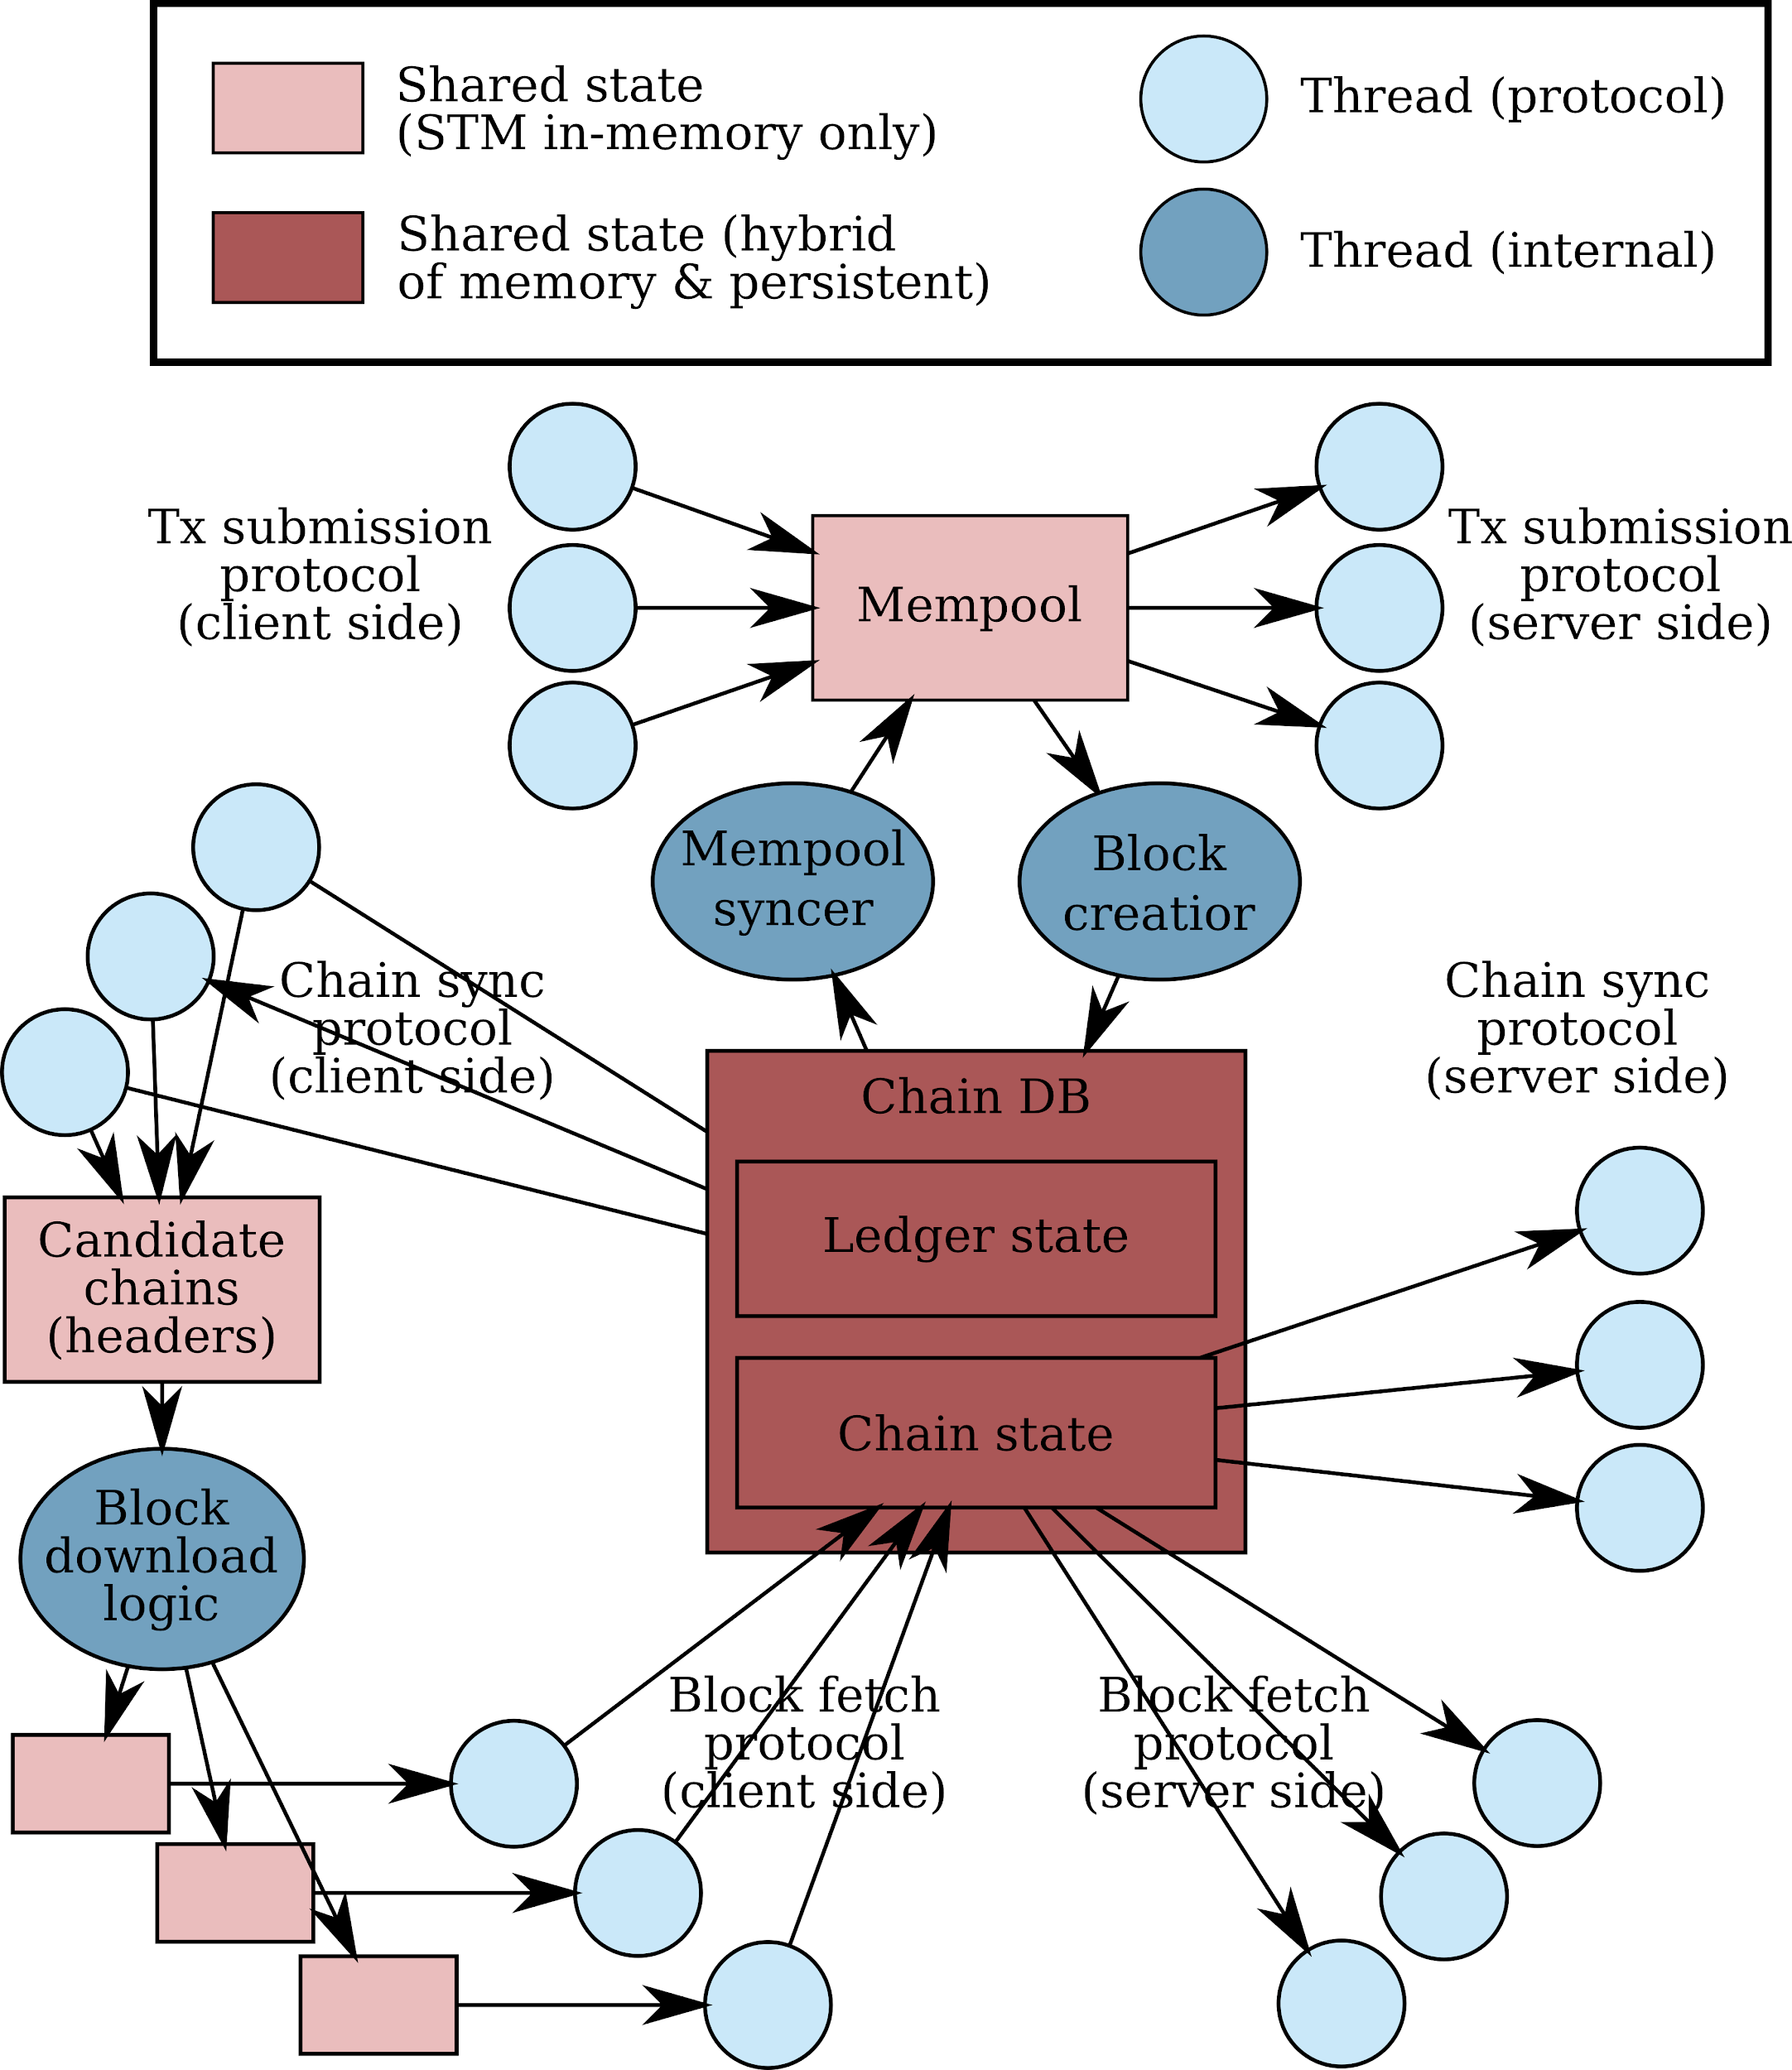
\includegraphics[width=6.27083in,height=7.25347in]{./media/image8.png}

The validation and chain selection functionalities of Ouroboros are in
four separate places:

\begin{enumerate}
\def\labelenumi{\arabic{enumi}.}
\item
  \begin{quote}
  Peer chain header validation is performed in the chain sync client.
  This covers all the Ouroboros chain validation protocol checks, but
  none of the checks on the block bodies.
  \end{quote}
\item
  \begin{quote}
  Initial selection of plausible chains takes place in the block fetch
  logic. It considers all the valid chains of headers maintained by the
  chain sync clients, and looks for ones that are longer than the
  current chain. It then picks one or more chains to download block
  bodies of. It picks on the basis of a combination of prioritising the
  longest chain, the available network resources and the expected
  ability to complete within deadlines. This should be considered part
  of chain selection.
  \end{quote}
\item
  \begin{quote}
  The evidence connecting the block header to the block body is checked
  by the block fetch client upon completing the download of the block
  body.
  \end{quote}
\item
  \begin{quote}
  The final block body (ledger) validation and chain selection are
  performed in a single integrated algorithm in the chain database.
  \end{quote}
\end{enumerate}

The fact that these are split up is deliberate. The checks are moved to
the earliest point in the operational cycle where the data is available,
and where the least resources have been expended. This helps build an
argument about bounded resource use and preventing asymmetric resource
attacks.

Some parts of the network layer are thus inherently specific to the
requirements of the consensus design\footnote{Though the implementation
  is highly parametric and can support the different protocol and ledger
  checks needed to implement many instances of the Ouroboros family.}, a
trade-off that is forced upon us by operating in an environment where
the adversary has so many cheap options\footnote{Again, contrast this
  with PoW where to get any higher than low-level network attacks using
  blocks, the adversary must provide a PoW which immediately shifts the
  resource argument in favour of the defenders.} but the other parts are
as general as reasonably possible. This provides more modularity and
flexibility and makes the code amenable to rigorous component level
testing and it also simplifies the review process (whether internal or
external).

\subsection{Network constraints and design decisions}
\label{network-constraints-and-design-decisions}

There is no clear line between the consensus and network layers of an
Ouroboros design. After all, Ouroboros itself is a high-level
message-based networked protocol. But generally speaking, the consensus
layer provides the \emph{policy} and the network layer provides the
\emph{mechanisms}:

\begin{itemize}
\item
  \begin{quote}
  The consensus layer handles issues deriving from the Ouroboros
  algorithm, whereas
  \end{quote}
\item
  \begin{quote}
  the network layer handles issues of effective use of network
  resources.
  \end{quote}
\end{itemize}

Both layers must be concerned with adversarial behaviour and asymmetric
resource attacks. The block fetch logic component is an exception in
that it has aspects of both layers: implementing parts of chain
selection, but also effective use of network resources.

The final high level consensus design has information exchange
requirements on three areas:

\begin{enumerate}
\def\labelenumi{\arabic{enumi}.}
\item
  \begin{quote}
  \emph{\textbf{chain sync}}: a requirement to support a stateful
  application-level protocol for synchronising chains of headers;
  \end{quote}
\item
  \begin{quote}
  \emph{\textbf{block fetch}}: a requirement for downloading block
  bodies; and
  \end{quote}
\item
  \begin{quote}
  \emph{\textbf{tx submission}}: a requirement for transmitting new
  transactions from the mempool in one node to that of another.
  \end{quote}
\end{enumerate}

\subsubsection{Stateful versus stateless protocols}
\label{stateful-versus-stateless-protocols}

Requirement 1 above (to support a stateful connection-oriented
application-level protocol) implies some notion of connection or
session.

This is straightforward by layering on top of a lower level
connection-oriented protocol, or as noted above, we could also add a
notion of session to a stateless protocol (at a price of more complex
resource management).

This design decision is discussed in
\cref{stateful-implementation}. The summary
is that there are not as many off-the-shelf solutions available as it
might first appear, since most protocol implementations are designed for
use within a data centre (thus within a controlled operational
environment) and not in the adversarial environment of the public
Internet. There does, however, exist a good stateful option: TCP; and
there is also a good stateless option: HTTP.

TCP and HTTP are common and well-supported, with robust and reliable
software libraries and tools. In terms of lines of code and maintenance
cost, there is little difference between approaches based on these two
protocols. Our chosen solution has two components layered on top of TCP,
each of which is less than 1000 lines of code.

To get to a roughly equivalent level of functionality with an
alternative solution (based on exclusively stateless application-level
protocols) on HTTP would likely involve picking existing libraries such
as "servant", that are built on top of the "wai" and "warp" HTTP server
stack. That would indeed save 2k lines of code, but there would then be
tens of thousands of extra lines of code to audit. There would also be
much more unnecessary functionality and network-exposed surface area for
attackers to exploit.

A further constraint stems from the business requirement to support
block-producing nodes on consumer-grade network connections. Such nodes
are usually behind firewalls. In practice this means they can only
establish outbound TCP connections, because inbound TCP connections are
blocked by the firewall. Protocols such as HTTP establish new TCP
connections for each new batch of requests, and those connections can
only be used for requests in one direction\footnote{HTTP persistent
  connections are a performance optimisation, and cannot be used for
  HTTP requests in the opposite direction. HTTP2 does allow some degree
  of server-push, but it is not a symmetric bi-directional connection.}.
This means that nodes behind firewalls can only make HTTP requests; they
cannot receive them. This places a general limitation on the design of
higher level consensus protocols, or requires a special asymmetric case
in the design to cope with such nodes. For example, in an RPC based
design layered on top of HTTP, RPC interactions can only be initiated by
the node behind the firewall. This

\begin{itemize}
\item
  \begin{quote}
  introduces an asymmetry into the design, and
  \end{quote}
\item
  \begin{quote}
  makes it harder to push notifications promptly, such as block header
  announcements, which puts ``home'' stake pools at a further
  disadvantage in meeting the Ouroboros timing constraints.
  \end{quote}
\end{itemize}

By comparison, with a bi-directional connection-oriented protocol such
as TCP, a connection can be established by the node behind the firewall
but once established the connection can be used in both directions. This
allows the application level protocols to be fully symmetric, which is
the natural design for a peer-to-peer rather than client/server system.

There are also significant advantages to being able to use stateful
application level protocols. Again, as noted above, stateful protocols
can rely on an amortised analysis for their resource bounds, which
simplifies the design of protocols that are (or can be made) resistant
to asymmetric resource attacks. For example, in an HTTP REST API, if
there is a moderately expensive operation that must be available to be
used as part of normal peer interactions then it is hard to mitigate an
attack where that API is used repeatedly -- without that mitigation also
affecting legitimate users of the API\footnote{For example through some
  form of rate limiting.}. In a stateful protocol that same interaction
can be tied to the previous actions of the same peer. This enables
mitigations that can add extra cost to the attacker, or can slow the
attacker down without slowing down other legitimate peers.

Ultimately, the choice of stateful or stateless chain synchronisation
protocol is a design decision on which reasonable people can and do
disagree. Maintenance costs are similar either way and both approaches
allow future flexibility, but

\begin{quote}
\emph{\textbf{this design decision in the consensus layer cannot easily
be changed later}}.
\end{quote}

The stateful chain sync pattern is relied upon in many parts of the
consensus design and implementation: the chain database, the peer
interactions and the local client IPC. Indeed, it is a unifying aspect
of the design that simplifies many aspects of the implementation.

An additional feature of adopting a contention-based, stateful
association with a peer is that, for the duration of that connection, we
can integrate information derived from that connection to inform local
decision making.

\subsubsection{Concurrency}
\label{concurrency}

Recall, from the beginning of
\cref{network-constraints-and-design-decisions}, that the consensus information exchange requirements cover three
areas: chain sync, block fetch and tx submission. Each relationship with
a direct upstream and downstream peer needs to cover all three areas,
however there is no requirement for any synchronisation between them
when talking to a single peer. They are independent when talking to
different peers, and at least semi-independent for a single peer.

Concurrency is of course a technique to structure programs in a modular
way, for those programs that need to interact with multiple external
agents {[}Marlow13, Chapter 1{]}. It is a natural design decision to use
concurrency for talking to independent peers. The same motivations lead
to the decision to handle the three areas (chain sync, block fetch and
tx submission) concurrently when talking to a single peer.

Using concurrency allows each of these three features to be handled in a
modular way. It results in three simple protocols rather than one
complex one, and a clear way to add new protocols or upgrade existing
ones. Chain sync, block fetch and transaction submission are independent
application-layer protocols that all run concurrently as required by the
consensus layer.

We thus end up with one Haskell thread per application-level protocol
per upstream and downstream peer. In extreme cases, this could be a
large number of threads but managing this is well within the
capabilities of the GHC runtime system {[}Marlow13, Chapter 15{]}.

\subsubsection{Bearer and multiplexing}
\label{bearer-and-multiplexing}

We must pick some underlying lower-level \emph{bearer} protocol over
which to run the collection of application-level protocols. Having
decided to support stateful application level protocols we must either
pick a stateful lower-level protocol or add session or connection
support to a stateless protocol. The clear and obvious choice is then to
use TCP. TCP is the best supported internet protocol when it comes to
the thorny issues surrounding consumer NAT and firewall hardware:
outbound TCP connections can almost always get through. It would be
plausible to use UDP-based options but that would either require
significant additional development work\footnote{And take on future risk
  as telecommunications start deploying
  \href{https://en.wikipedia.org/wiki/Carrier-grade_NAT}{{Carrier Grade
  Nat}} to migitage IPv4 address exhaustion.}, or it would be necessary
to rely on some relatively new UDP-based protocols with immature
implementations. Similarly, adding sessions to another higher level
protocol such as HTTP would add complexity, but would have little
benefit.

The only significant drawback of selecting TCP is that we wish to run
multiple application level message-based protocols with a single peer
concurrently, whereas TCP supports a \emph{single} reliable ordered byte
stream. Adapting stream-based communication to provide message-based
communication just needs simple \emph{framing}. To support concurrent
protocols requires either using multiple TCP connections or else running
the collection of protocols over a single TCP connection. Using multiple
TCP connections requires more resources\footnote{Kernel buffers,
  file/socket handles etc.} and also has other disadvantages such as
more complexity in fully disconnecting from a peer that is deemed to be
adversarial.

The standard solution to this well-known networking problem is to use
multiplexing. That is, at one end we multiplex by chopping up the data
streams from the individual protocols into bounded sized chunks and
interleave them on the single TCP data stream, and at the other end we
demultiplex to reverse the transformation. The abstraction that is
presented by the multiplexer is essentially the same as that of TCP
itself: a reliable ordered byte stream. This is described in more detail
in the \cref{network-mux}.

\subsubsection{Performance}
\label{performance}

Performance is a very important consideration for the network layer,
deriving from:

\begin{enumerate}
\def\labelenumi{\arabic{enumi}.}
\item
  \begin{quote}
  the Ouroboros timing constraints;
  \end{quote}
\item
  \begin{quote}
  the business requirements to support certain latencies and
  throughputs;
  \end{quote}
\item
  \begin{quote}
  the business requirement to support worldwide distribution; and
  \end{quote}
\item
  \begin{quote}
  the requirement to support block-producing nodes on consumer-grade
  network connections.
  \end{quote}
\end{enumerate}

In the context of networks, performance amounts primarily to trying to
use the network resource effectively whenever possible. Time that is
expended without sending or receiving data is time that can never be
regained. Point-to-point connections over a network can very
crudely\footnote{A much more precise characterisation is based on $\Delta{}Q$,
  see {[}Comp20{]}.} be characterised as having a certain bandwidth and
latency. Network connections do not support bursts of traffic well,
since they have a maximum bandwidth. Full network utilisation requires
that they be used at their maximum bandwidth continuously.

Network latency poses a significant challenge to effectively utilising a
network connection, and this challenge tends to leak all the way up to
the application-level protocols and application design. Network
latencies also vary considerably, with many orders of magnitude
difference between peers within a data center versus peers on other
continents (see \cref{tcp-rpc-response-behavior}). Catering for this very wide range of latencies requires
careful design. Ideally, protocols should be capable of adapting to the
latency that is actually experienced, rather than being targeted to a
specific latency.

There are two major approaches to dealing with network latency:
\emph{batching} and \emph{pipelining}. Batching amounts to sending a
large amount of data in one logical interaction, for example requesting
a multi-megabyte file over HTTP. This hides latency in the sense that
the full end-to-end round trip is amortised over the amount of data
moved. Batching is relatively easy to implement, though it does require
changes in the application level protocols. Moreover, picking the right
batching size requires some care and thus becomes an application level
concern. Batching by itself cannot fully utilise a network connection on
a continuous basis due to the need to wait for the end of each batch.
This improves as the batch size gets bigger, but there are also negative
trade-offs with large batch sizes. By contrast, a fully pipelined
protocol can fully saturate a network connection. Pipelining involves
sending multiple messages back to back without waiting for replies, and
handling replies as they come in. The primary disadvantage of pipelining
is that it tends to complicate the data flow and control flow in the
application\footnote{Surprisingly few HTTP client applications take
  advantage of HTTP pipelining for example.}.

\subsubsection{Binary formats}
\label{binary-formats}

We must choose an encoding format for messages in the protocols. Choices
include

\begin{itemize}
\item
  \begin{quote}
  standardised text formats like JSON, and
  \end{quote}
\item
  \begin{quote}
  standardised binary formats like ASN.1, MsgPack, CBOR and those used
  by Thrift and ProtoBufs.
  \end{quote}
\end{itemize}

The implementation (not just the encoding format) must be robust against
untrusted input from the network. Further considerations, in
roughly\footnote{The order is of course somewhat a matter of opinion,
  and it by no means implies a strict lexicographical order for
  evaluating different choices.} decreasing order of importance,
include:

\begin{enumerate}
\def\labelenumi{\arabic{enumi}.}
\item
  \begin{quote}
  standardised format or not
  \end{quote}
\item
  \begin{quote}
  stability of standard
  \end{quote}
\item
  \begin{quote}
  availability of format documentation
  \end{quote}
\item
  \begin{quote}
  availability of existing implementations
  \end{quote}
\item
  \begin{quote}
  availability of existing implementations for 3rd party implementations
  \end{quote}
\item
  \begin{quote}
  availability of existing support tools
  \end{quote}
\item
  \begin{quote}
  having a schema language for documentation and validation
  \end{quote}
\item
  \begin{quote}
  availability of schema tools
  \end{quote}
\item
  \begin{quote}
  ease of forwards/backwards compatibility
  \end{quote}
\item
  \begin{quote}
  encoding size
  \end{quote}
\item
  \begin{quote}
  performance of encoding and decoding
  \end{quote}
\item
  \begin{quote}
  minimising excessive code dependencies
  \end{quote}
\end{enumerate}

There are several perfectly adequate choices that score well against all
the criteria, including one -- CBOR
(\href{https://tools.ietf.org/html/rfc7049}{{RFC 7049}}) -- that is
already in use in the system as the binary format for the blockchain
itself that scores well on all the criteria\footnote{Thrift and
  ProtoBufs do score better on the support tools, particularly schema
  tools, but the CBOR schema schema language is standardised (as
  \href{https://tools.ietf.org/html/rfc8610}{{RFC 8610}}) and the
  validation tools are adequate and are already used in the CI tests for
  the new Cardano implementation.}. eusing the same choice leads to
significant savings:

\begin{itemize}
\item
  \begin{quote}
  reduces dependencies,
  \end{quote}
\item
  \begin{quote}
  simplifies documentation,
  \end{quote}
\item
  \begin{quote}
  reduces the cognitive load for developers,
  \end{quote}
\item
  \begin{quote}
  reduces audit costs, and
  \end{quote}
\item
  \begin{quote}
  minimises the maintenance burden.
  \end{quote}
\end{itemize}

This is true for the present Cardano implementation and any other
compatible implementation. The present implementation uses an existing
Haskell CBOR implementation that has been tested and externally audited
to deal robustly with untrusted input.

\subsection{Network libraries and components}
\label{network-libraries-and-components}

Following from the high-level design choices above, the network layer
design consists of the following libraries and components:

\begin{itemize}
\item
  \begin{quote}
  A \emph{multiplexer} component that carries multiple concurrent
  reliable ordered streams over a single reliable ordered bearer such as
  TCP\footnote{It can use any reliable ordered bearer connection.This
    greatly aids testing, but also adds flexibility.}.
  \end{quote}
\item
  \begin{quote}
  The \emph{typed-protocols} framework for describing and using
  application level protocols, with enforcement via Haskell types. This
  is a form of \href{https://groups.inf.ed.ac.uk/abcd/}{{session
  typing}}. It also has direct support for pipelining. It is described
  in more detail in this section below.
  \end{quote}
\item
  \begin{quote}
  An \emph{IO simulator} library was developed for the purpose of
  testing the network and consensus components. It is described in more
  detail in this section below.
  \end{quote}
\item
  \begin{quote}
  The three application level protocols (node to node):
  \end{quote}

  \begin{itemize}
  \item
    \begin{quote}
    chain sync;
    \end{quote}
  \item
    \begin{quote}
    block fetch; and
    \end{quote}
  \item
    \begin{quote}
    tx submission.
    \end{quote}
  \end{itemize}
\end{itemize}

\begin{quote}
These define the mechanism but not the policy for using these protocols.
They are defined using the typed-protocols framework.
\end{quote}

\begin{itemize}
\item
  \begin{quote}
  A \emph{connection handshake} protocol used during the initial set-up
  of connections with peers. It covers protocol version negotiation and
  checking compatibility of parameters like the network magic\footnote{This
    provides early failure and feedback when nodes accidentally connect
    to the wrong network, e.g. testnet vs mainnet.}. This is also
  defined using the typed-protocols framework.
  \end{quote}
\item
  \begin{quote}
  A \emph{subscription manager} component that decides when to make new
  outbound connections to peers, which peers to connect to, and handles
  the process of doing so.
  \end{quote}
\item
  \begin{quote}
  A \emph{server} component that handles accepting and managing inbound
  connections from other peers.
  \end{quote}
\item
  \begin{quote}
  A \emph{block fetch} component. This was also listed as a consensus
  component but because it incorporates many concerns from the network
  layer such as achieving good network performance it was developed by
  the network team and is included within the network layer package. As
  mentioned previously this is a relatively sophisticated concurrent
  component: it selects plausible candidate chains based on the
  available valid chains of headers, and decides which block bodies to
  download from which peers. It provides the policy for the block fetch
  protocol.
  \end{quote}
\item
  \begin{quote}
  A \emph{local tx submission protocol} which is tailored to local
  clients (wallets, explorers, etc.). Since it runs in a trusted
  environment it can be simpler, which reduces implementation complexity
  for clients. It also gives immediate verbose feedback to a client
  application on tx validation failures.
  \end{quote}
\item
  \begin{quote}
  A \emph{chain fragment} module that is shared with the consensus
  layer. It defines an in-memory data structure for dealing efficiently
  with sub-sequences of blockchain headers.
  \end{quote}
\end{itemize}

As described in the previous section, the multiplexer satisfies the need
to run multiple independent application level protocols concurrently
over a single TCP connection\footnote{While avoiding issues of ``TCP
  Meltdown'' (running
  \href{https://en.wikipedia.org/wiki/Tunneling_protocol\#Secure_Shell_tunneling}{{TCP
  over TCP}})}. It is perhaps worth noting that multiplexing is not
unusual: the old cardano-sl network implementation also relied on a
multiplexer as part of the network-transport-tcp package. The new
implementation is simpler, smaller, more modular, and a better fit for
the new design requirements.

We have the requirement
(\cref{network-connectivity}) that small
stakeholders with reasonable consumer-grade network connections and
equipment should be able to operate a stake pool. This translates to the
technical requirement that nodes behind firewalls should be able to take
part without having to make manual alterations to their firewall
configuration. To satisfy this, the design relies on establishing
outbound TCP connections and then using the connections in a
bi-directional manner.

We have the requirement to support multiple application level protocols
and to bridge the gap between the reliable ordered byte stream
abstraction presented by the multiplexer and the reliable ordered
message stream required by application level protocols. We must also
make effective use of network resources, and must do it all in a way
that respects the constraints stemming from the adversarial environment.
This collection of requirements is met by the typed-protocols library
developed for the purpose. It meets the requirements and brings with it
a simple conceptual framework for thinking about and describing
application level protocols.

The typed-protocols library is the jewel in the crown\footnote{It is a
  session type framework. Session types are actively researched for more
  than 20 years, see {[}H93, THK94, HVK98{]}, and various
  implementations exists:
  \href{http://www.dcs.gla.ac.uk/research/mungo/}{{Mungo}} (Java),
  \href{http://www.scrible.org}{{Scrible}}, or {[}MV11{]} (Erlang), and
  many others.} of the network layer implementation and it has already
been presented at three public events\footnote{Notably at the
  \href{https://monadic.party/\#talks}{``Monadic Party'' 2019 Haskell
  Summer School, Poznan, PL}, and at the
  \href{https://skillsmatter.com/conferences/11741-haskell-exchange-2019\#program}{{``Haskell
  eXchange'' 2019}} London.}. It casts application level protocols in
the form of state machines with the constraint that both peers agree on
the state that they are in. The transitions between states correspond to
messages sent between the peers, so the protocol state dictates which
messages may be sent or received. A further constraint is that each
protocol state is labeled with the peer that has agency to send messages
in that state. Thus in each protocol state one peer may send any message
(valid for the state) and the other peer must accept any valid message
(valid for the state). These constraints impose some simplicity on the
application level protocols and make the protocols deadlock-free by
construction. The library allows encoding protocols of this form in
Haskell types, and thereby enforcing at compile time that
implementations of the protocols comply with the constraints implied by
the protocol state machines. In combination with compiler warnings it
ensures that protocols only send when they are allowed to and only
messages appropriate for the state, and conversely are prepared to
receive when required and will handle all the messages allowed for the
state. This provides structure to help writing protocol implementations.

Performance is a major consideration for the protocol design, as
discussed in the previous section. The typed-protocols library has an
innovative and effective solution. Many protocols of interest, including
the three consensus protocols, can be pipelined \emph{without any change
to the protocol state machine}. The library provides a way to write a
protocol implementation in a pipelined way, with the exact same
protocol-compliance guarantee enforced by the types. Indeed it also
provides type safety for certain pipelining invariants which is
immensely helpful for writing pipelined implementations. The pièce de
résistance is that a pipelined client can be paired up against a
``normal'' server that is oblivious to pipelining with the result being
a pipelined use of the protocol. This makes using pipelining pervasively
a very tractable proposition, and all three consensus protocols have
fully pipelined implementations.

The individual consensus protocols are each designed with a few
constraints and qualities in mind. They are designed:

\begin{itemize}
\item
  \begin{quote}
  to allow implementations that can work in bounded space;
  \end{quote}
\item
  \begin{quote}
  to maximise the opportunities for pipelining;
  \end{quote}
\item
  \begin{quote}
  to exclusively use consumer driven control flow, without polling;
  \end{quote}
\item
  \begin{quote}
  to be highly parametric to maximise flexibility and simplify testing;
  \end{quote}
\item
  \begin{quote}
  to otherwise minimise the complexity of protocol implementations.
  \end{quote}
\end{itemize}

The motivations for these are all obvious except perhaps the consumer
driven control flow. The motivation here is again about resource use. To
avoid overload, malicious or otherwise, the consumer should decide when
it is ready to accept new information to process. This does not prevent
prompt transmission of, for example, new headers or transactions, and no
costly polling is required. This fits naturally in a stateful protocol.

The IO simulator was developed to aid testing. It is used in tests for
network components, individual protocols, application level protocol
implementations, components within the consensus layer, and the
combination of the network and consensus layers as a whole. It provides
deterministic execution of concurrent code. It can produce a trace of
interesting execution events. This is useful because many properties of
concurrent code we wish to test are expressed in terms of event traces.
It provides faster than real time simulation of time delays which is
helpful for testing network protocol timeouts. It will in future allow
testing consensus between nodes with clocks that are not completely in
sync, which is otherwise a very awkward test to set up and run
automatically.

The bulk of the code in the network and consensus implementations are
parameterized over the type classes from the io-sim-classes package,
which enables running \emph{precisely the same} code in IO for
production or in the IO simulator for testing. For example the consensus
storage subsystem is tested this way with simulated I/O failures and
file corruption.

\subsection{Related work (data diffusion)}
\label{related-work-data-diffusion}

As discussed in
\cref{interleaving-transmission-and-validation}, there are strong reasons to conclude that pure broadcast cannot
be used in any Ouroboros implementation that respects the Ouroboros
threat model, and reasons to conclude that modifying a broadcast
algorithm with the necessary checks is not a reasonable engineering
trade-off. This excludes many implementations of broadcast, including
multicast and pub/sub (publish/subscribe) algorithms.

\subsubsection{PolderCast}
\label{poldercast}

PolderCast {[}SSVV12{]} is an implementation of pub/sub. As such it is
not useful for an implementation of Ouroboros data diffusion as
discussed in
\cref{interleaving-transmission-and-validation}, (namely the asymmetry in favour of adeversies). PolderCast,
however, also establishes a P2P graph which is a necessary feature of a
fully distributed Cardano implementation. This is discussed in summary
in \cref{related-work-decentralisation} and PolderCast is considered in
more detail in \cref{poldercast-1}.

\subsubsection{Other blockchain systems}
\label{other-blockchain-systems}

Significant related work is the data diffusion function of other
existing (PoW) blockchain systems. As discussed in
\cref{interleaving-transmission-and-validation}, PoW provides a balance between adversaries and honest nodes
that allows such systems to use broadcast algorithms (at least for block
headers) modified with a stateless verification filter. PoW systems are
also typically asynchronous, unlike Ouroboros which must ensure block
delivery within deadlines.

Bitcoin, Ethereum and the previous Cardano implementation are considered
in more detail in
\cref{comparison-with-previous-network-implementations}.

\subsubsection{Other related work}
\label{other-related-work}

Much related work exists on the choice of lower level network protocols.
HTTP and the issue of stateless protocols was discussed in
\cref{stateful-versus-stateless-protocols}
and is also discussed in
\cref{stateful-implementation}.

Other stateful protocol layers include libraries such as ZeroMQ or
servers for message queue protocols like AMQP such as RabbitMQ.
Unfortunately, as discussed in
\cref{stateful-implementation} the widely
used choices are not designed to be used on the public internet.

The \href{https://martinfowler.com/eaaDev/EventSourcing.html}{{event
sourcing architecture}} is however a direct inspiration for the
architecture for the Cardano node. This architectural style is designed,
amongst other things, to achieve very loose coupling in distributed
applications. In particular, the relationship between the node as a data
source and local node clients as data consumers is directly based on
this idea. The key impediment to reusing implementations, rather than
just ideas, is the fact that blockchain algorithms only provide eventual
finality rather than instant finality.

UDP is a lower-level internet protocol than TCP. TCP was chosen versus
UDP because TCP delivers the appropriate bearer characteristics needed
for the mini-protocols, is supported in all firewalls and has tried and
tested methods for dealing with IP packet fragmentation. This is however
a decision that would be reasonable to revisit in future.

Establishing connections between consumer nodes that are both behind
firewalls is difficult but it would enable nodes on consumer broadband
to make a greater contribution to the P2P network. Further research
would be required to evaluate potential solutions, but a solution may
involve augmenting the system with an additional non-TCP based bearer
protocol specifically for use between nodes behind firewalls.

The typed-protocols library can be considered as a limited and very
lightweight form of session typing. Related work is thus the existing
literature on session types. The
\href{https://groups.inf.ed.ac.uk/abcd/}{{ABCD project}}, in which
Professor Wadler is involved, maintains a large collection of references
and other resources.

\subsection{Decentralisation constraints}
\label{decentralisation-constraints}

The requirements for decentralisation come from a combination of the
business requirements and technical requirements deriving from
Ouroboros. The business requirements are set out in
\cref{business-requirements}. The dominant
constraints derive from the nature of reality and from characteristics
of the Internet as it currently exists. We will review the key
requirements and constraints.

Ouroboros is a system with hard real-time deadlines. They are deadlines
measured in seconds, not microseconds, but they are deadlines
nevertheless. The deadlines can be missed from time to time by eating
into the adversarial stake budget, but consistent failure to meet the
deadlines destroys the properties of the system\footnote{Praos does make
  this better in that it becomes a gradual degradation rather than a
  cliff edge. This lets it cope better with variance in block delivery
  times, but it does not help substantially with the whole distribution
  being shifted.}. We get to pick the exact numbers for slot times or
block sizes, but whatever values we pick, we must be able to keep to the
deadlines in the vast majority of cases. IOHK's Chief Scientist Aggelos
Kiayias set a practical target of achieving the deadline in 95\% of
cases. Compare this, for example, with a PoW system such as Ethereum,
which is an asynchronous system without hard deadlines. It can be, and
has been, adjusted over time, with longer block times during periods of
high load (see \cref{ethereum} for
details). This is not an option for Ouroboros as it exists now: we must
pick the slot length parameter and we have no mechanism to adjust it on
short time scales in response to network events. If we pick too relaxed
a target then we leave transaction throughput on the table, and too
tight a target risks system collapse. Thus a clear priority is
\emph{consistency} of block delivery times. We wish to avoid a long
tail\footnote{See \cref{bitcoin} which
  touches on an analysis of the Bitcoin network and the long tail of
  block delivery times}.

The other key business requirements are:

\begin{itemize}
\item
  \begin{quote}
  the network layer should be decentralised in the sense that "IOHK
  should be in the same position on the network as any other stakeholder
  with an equivalent amount of stake";
  \end{quote}
\item
  \begin{quote}
  to support certain transaction latencies and throughput rates;
  \end{quote}
\item
  \begin{quote}
  to support worldwide distribution;
  \end{quote}
\item
  \begin{quote}
  1,000 stakepool nodes holding about 80\% of the system's
  stake\footnote{The original business requirement was for 100
    large-scale stake pools (see
    \cref{participate-in-network-as-a-large-stakeholder}) but this was
    later raised to 1000.};
  \end{quote}
\item
  \begin{quote}
  10,000 other small-scale private stakepool nodes; and
  \end{quote}
\item
  \begin{quote}
  the requirement to support private stake pools operating on
  consumer-grade network connections;
  \end{quote}
\end{itemize}

There is a trade-off between block size and the transmission time of a
block from one slot leader to the next. Of course the bigger the blocks
that can consistently be delivered within the deadline, the higher the
transaction throughput. The interesting question is how well we can do
within this trade-off: can we easily meet the TPS targets or is this a
harder problem? If the problem is easy then we may be able to use
off-the-shelf solutions that do not get the highest possible TPS but at
least cover the TPS targets. If the constraints make the problem more
difficult then we may require a customised solution simply to hit our
TPS targets. Thus we should review the factors that may impinge on
transferring blocks of various sizes across a network, since that
determines the envelope within which we can adjust the block size versus
transmission-time trade-off.

In general the consensus nodes must arrange themselves in a graph. It
does not scale very far to have every node linked to every other node.
To work in limited memory and network resources we must limit the
\emph{valency} for each node -- that is each graph node's in-degree or
out-degree. This means that in general a block must transit multiple
hops through the graph to get from one slot leader to the next. Since we
are interested in the overall transmission time between slot leaders
then we must be interested in both the number of hops and the
transmission time on each hop. A useful technical graph metric here is
one known as the characteristic path length (see
\cref{characteristic-path-length}). Informally it can be thought of the
typical path length, taking into account both the number of hops and
the hop transmission times.

Let us consider the number of hops. The typical number of hops clearly
depends on the size of the graph, the typical valency and the shape of
the graph. \cref{model-of-network-scaling}
provides tables relating hop counts and valencies with maximum graph
size (at least in the perfect case of a homogeneous spanning tree). This
tells us that for our target of 1000 stake pools, related relay nodes,
and other participants, we can expect to have a hop count of at least 5
and a valency of 5 or more. This valency appears reasonable, though in
reality it cannot be homogeneous. We would hope to allow edge nodes to
use a lower valency and server-class nodes to be able to support a
substantially higher valency.

Let us consider the transmission time per hop. This clearly depends on
the characteristics of the Internet and of TCP, the underlying transport
protocol that we use.
\cref{tcp-rpc-response-behavior} presents
tables of transmission delays based on a model of TCP, calibrated with
measurements between AWS data centres in various regions. For larger
block sizes, such as 1Mb, the transmission times for intercontinental
hops become quite large, in the 0.5--2.5 second range. Transmission
times in this range are a significant fraction of our overall slot
length budget.

The conclusion from the per-hop transmission time numbers is that if we
are to use larger block sizes then we will need to ensure that on a
typical path we do not get too many intercontinental hops. This can be
ensured either by keeping the overall hop count low, or by selecting
hops in a way that is sensitive to their transmission delays (or of
course a combination). We already know, however, that we must expect hop
counts of at least five, and five intercontinental hops brings us
perilously close to our overall slot time budget once one takes into
account other delays such as processing time, clock skews and other
factors mentioned in \cref{timeliness-constraint}. So this suggests that at least for larger block sizes, we are
not in the "easy" scenario since we must keep both hop count and hop
transmission times under control.

How large must the blocks be to hit our TPS targets? This is a
straightforward calculation.
\cref{fundamental-tradeoffs} has a table
relating average transaction size, block size and TPS, for 20s slot
times. For example, for 1kb (kilobyte) transactions, 50 TPS requires 1Mb
(megabyte) blocks. In the existing Byron system the smallest practical
transactions are over 350 bytes, while exchanges chafe at the 8kb
transaction size limit, and new features such as metadata, multi-sig and
scripts will all require larger transactions.

Once we take into account future user base growth and the expected
growth in transaction sizes then our conclusion must be that if we wish
to scale to our stretch goals, or perhaps even to hit our target goals,
we must use a decentralised P2P graph construction mechanism that is
sensitive to the combination of path hop counts and hop transmission
times. Or conversely, we can only be oblivious of hop transmission times
if we have small block sizes and hence low overall throughput.

Ideally any design we pick now should be one where we can have
confidence that we can meet conservative initial throughput goals, but
that does not preclude scaling to more users, higher throughputs etc.

A threat that is of significant concern in existing distributed
blockchain systems is that of \emph{eclipse} attacks. An eclipse attack
is where attackers try to insert themselves in the network graph in such
a way as to prevent a target node from discovering the "true" blocks
from the system. To prevent the target node from becoming aware that it
is eclipsed, the typical approach is for the attackers to supply the
target with their own valid chain.

Eclipse attacks are a relevant problem for PoW blockchain systems. The
crucial difficulties for PoW systems appear to be these:

\begin{itemize}
\item
  \begin{quote}
  attackers (with moderate hashing power) executing an eclipse attack
  can create growing -- albeit slowly growing -- valid chains; and
  \end{quote}
\item
  \begin{quote}
  a node does not generally know the amount or distribution of hashing
  power.
  \end{quote}
\end{itemize}

Ouroboros does not share these difficulties. While it remains the case
that attackers (with moderate stake) attempting to execute an eclipse
attack can create valid slowly-growing chains, the difference is that
validating nodes inherently know the current stake distribution. The
node that is the target of the attack can compare the chain it observes
with the current stake distribution and gather probabilistic evidence
that it is being eclipsed.
\cref{performance-model-of-ouroboros-praos}
provides an analysis of the speed and confidence with which this can be
established. The conclusion is that at least for low stake attackers the
time scales are very practical. More analysis is needed for medium and
high stake attackers. Our threat model dictates that we must at least
handle low stake adversaries.

\subsection{Decentralisation design}
\label{decentralisation-design}

Analysis of ``S/Kademlia'' suggests that one of the main drivers for its
complex design is that it attempts to establish a degree of resistance
to eclipse attacks based on very weak assumptions. It appears that
starting from so few assumptions makes it difficult to establish
resistance to eclipse attacks. As described above, however, Ouroboros
furnishes us with the ability to probabilistically detect eclipse
attacks on relatively short time scales. It is also worth noting that a
deliberate eclipse attack and an accidental network partition are
essentially identical from the perspective of the victims. Thus a
solution that can \emph{recover} from eclipse attacks already has many
of the characteristics needed to recover from accidental
partitions\footnote{The consideration of the appropriate mitigations to
  large scale network disruption (e.g. BGP routing issues, undersea
  cable damage) including their likely time to repair etc is part of the
  planned work.}.

In our use case we must build a large graph in a decentralised way,
initially from nodes contributed by IOHK and later by state pool
operators, and grow it to support all stake pools and users. We would
like small hop counts and we would also like to avoid the danger of
there being too many long hops.

A literature review did not reveal existing complete designs that could
meet the combination of timing and throughput goals, when scaled up to
the expected number of nodes, when globally distributed, and subject to
the behaviour of TCP\footnote{Using TCP is not a theoretical constraint,
  but it is a practical engineering and development schedule constraint.}.
Selected related work is discussed in the next section, and the
constraints are analysed in more detail in
\cref{timeliness-constraint} and
\crefrange{tcp-rpc-response-behavior}{time-synchronisation-constraints}.
The literature review does however reveal useful theory.

Graph theory {[}Watts99{]} tells us that small hop counts\footnote{This
  research provides a basis for the pre-existing popular "small world"
  idea of
  \href{https://en.wikipedia.org/wiki/Six_degrees_of_separation\#Computer_networks}{{six
  degrees of separation}}.} (formally, the characteristic path length)
can be achieved in large graphs, including random graphs. Furthermore it
tells us that these graphs can be "grown" from smaller ones. This is a
very helpful combination of characteristics for our use case, as we want
small hop counts, and random graphs are easier to build in a
decentralised way than highly structured ones, especially in the
presence of failures and adversarial behaviour. To achieve the low
characteristic path length, the theory requires that nodes have a high
enough mean valency, and a high enough standard deviation in the
valency. Under these conditions the low characteristic path length is
remarkably stable -- for a range of starting graph types including
random graphs\footnote{Interestingly, rings are a pathological starting
  case}. Typical numbers are a mean of 10 and standard deviation of 3,
which give a rough range of valencies of 4--16. This would appear to be
eminently achievable, using the middle of the range for edge consumer
nodes, and using the upper end for server nodes.

Bearing in mind the requirements, constraints and theory, our approach
is to solve the problem directly, using a single simple flexible design.

The theory tells us that we can use random graph construction, which we
can do with standard \emph{random gossip} techniques. This deals with
the decentralisation requirement and the low hop count constraint. The
remaining significant issues are avoiding eclipse attacks, as previously
discussed, and avoiding too many long hops. Our design is to augment
random gossip with two layers of control loop to address these two
issues. This general design is relatively simple, and has the
significant virtue that the policy for the control loops can be adjusted
after initial deployment with relatively few compatibility impacts. This
should enable the policy to be optimised based on real-world feedback,
and feedback from simulations of scale or scenarios that are hard (or
undesirable) to test in a real deployment.

Each node maintains three sets of known peer nodes:

\begin{itemize}
\item
  \begin{quote}
  \textbf{cold peers} are peers that are known of but where there is no
  established network connection;
  \end{quote}
\item
  \begin{quote}
  \textbf{warm peers} are peers where a bearer connection is established
  but it used only for network measurements and is not used for any
  application level consensus protocols;
  \end{quote}
\item
  \begin{quote}
  \textbf{hot peers} are peers where the bearer connection is actively
  used for the application level consensus protocols.
  \end{quote}
\end{itemize}

Limited information is maintained for these peers, based on previous
direct interactions. For cold nodes this will often be absent as there
may have been no previous direct interactions. This information is
comparable with "reputation" in other systems, but it should be
emphasised that it is purely local and not shared with any other node.
It is not shared because this is not necessary and because establishing
trust in such information is difficult and would add additional
complexity. The information about peers is kept persistently across node
restarts, but it is always safe to re-bootstrap -- as new nodes must do.

For an individual node to join the network, its bootstrapping phase
starts by contacting root nodes and requesting sets of other peers,
which are added to the cold peer set. It proceeds iteratively by
randomly selecting other peers to contact to request more known peers.
This gossip process is governed by a control loop that has a target to
find and maintain a certain number of cold peers. Bootstrapping is not a
special mode, rather it is just a phase for the control loop following
starting with a cold peers set consisting only of the root nodes. This
gossiping aspect is closely analogous to the first stage of Kademlia,
but with random selection rather than selection directed towards finding
peers in an artificial metric space.

The root nodes used in the bootstrapping phase are the stakepool relays
published in the blockchain as part of the stakepool registration
process. See the
\href{https://hydra.iohk.io/job/Cardano/cardano-ledger-specs/delegationDesignSpec/latest/download-by-type/doc-pdf/delegation_design_spec}{{Shelley
delegation design specification, Sections 3.4.4 and 4.2}}. As with
Bitcoin, a recent snapshot of this root set must be distributed with the
software.

The inner control loop governs the following activities:

\begin{itemize}
\item
  \begin{quote}
  the random gossip used to discover more cold peers;
  \end{quote}
\item
  \begin{quote}
  promotion of cold peers to be warm peers;
  \end{quote}
\item
  \begin{quote}
  demotion of warm peers to cold peers;
  \end{quote}
\item
  \begin{quote}
  promotion of warm peers to hot peers; and
  \end{quote}
\item
  \begin{quote}
  demotion of hot peers to warm peers.
  \end{quote}
\end{itemize}

The inner control loop has the following goals to establish and
maintain:

\begin{itemize}
\item
  \begin{quote}
  enough cold peers (e.g. 1000);
  \end{quote}
\item
  \begin{quote}
  enough hot peers to meet the valency target (e.g. order of 5--20);
  \end{quote}
\item
  \begin{quote}
  enough warm peers in total (e.g. order of 10--50)
  \end{quote}
\item
  \begin{quote}
  a set of warm peers that are sufficiently diverse in terms of hop
  distance.
  \end{quote}
\item
  \begin{quote}
  a target churn frequency for hot/warm changes
  \end{quote}
\item
  \begin{quote}
  a target churn frequency for warm/cold changes
  \end{quote}
\item
  \begin{quote}
  a target churn frequency for cold/unknown changes
  \end{quote}
\end{itemize}

The target churn values are adjusted by the outer control loop, which we
will address below.

Local static configuration can also be used to specify that certain
known nodes should be selected as hot or warm peers. This allows for
fixed relationships between nodes controlled by a single organisation,
such as a stake pool with several relays. It also enables private
peering relationships between stake pool operators and other likely
deployment scenarios.

Using 5--20 hot peers is not as expensive as it might sound. Keep in
mind that only block headers are sent for each peer. The block body is
typically only requested once. It is also worth noting that the block
body will tend to follow the shortest paths through the connectivity
graph formed by the hot peer links. This is because nodes will typically
request the block body from the first node that sends the block header.

While the purpose of cold and hot peers is clear, the purpose of warm
peers requires further explanation. The primary purpose is to address
the challenge of avoiding too many long hops in the graph. The random
gossip is oblivious to hop distance. By actually connecting to a
selection of peers and measuring the round trip delays\footnote{Or more
  precisely the two unidirectional $\Delta{}Q$ measures} we can start to
establish which peers are near or far. The policy for selecting which
warm peers to promote to hot peers will take into account this network
hop distance. The purpose of a degree of churn between cold and warm
peers is, in part, to discover the network distance for more peers and
enable further optimisation or adjust to changing conditions. The
purpose of a degree of churn between warm and hot peers is to allow
potentially better warm peers to take over from existing hot peers.

The purpose in maintaining a diversity in hop distances is to assist in
recovery from network events that may disrupt established short paths,
such as internet routing changes, partial loss of connectivity, or
accidental formation of cliques. For example, when a physical
infrastructure failure causes the short paths to a clique of nodes to be
lost, if some or all of the nodes in that clique maintain other longer
distance warm links then they can quickly promote them to hot links and
recover. The time to promote from warm to hot need be no more than one
network round trip.

Overall, this approach follows a common pattern\footnote{Simulated
  annealing for example} for probabilistic search or optimisation that
uses a balance of local optimisation with some elements of higher order
disruption to avoid becoming trapped in some poor local optimum.

The local peer reputation information is also updated when peer
connections fail. The existing implementation classifies the exceptions
that cause connections to fail into three classes:

\begin{itemize}
\item
  \begin{quote}
  internal node exceptions e.g. local disk corruption\footnote{The
    recovery from detected disk corruption involves resetting to a
    known-good state, which involves shutting down connections to all
    peers.};
  \end{quote}
\item
  \begin{quote}
  network failures e.g. dropped TCP connections; and
  \end{quote}
\item
  \begin{quote}
  adversarial behaviour, e.g. a protocol violation detected by the
  typed-protocols layer or by the consensus layer.
  \end{quote}
\end{itemize}

In the case of adversarial behaviour the peer can immediately be demoted
out of the hot, warm and cold sets. We choose not to maintain negative
peer information for extended periods of time; to bound resources and
due to the simplicity of Sybil attacks.

The outer control loop deals with the problem of eclipse -- whether
malicious or accidental -- and also adjusts the behaviour of the inner
control loop over longer time scales. The outer control loop controls:

\begin{itemize}
\item
  \begin{quote}
  the target churn frequencies of the inner control loop for
  promotion/demotion between the cold/warm/hot states
  \end{quote}
\item
  \begin{quote}
  partial or total re-bootstrapping under certain circumstances
  \end{quote}
\end{itemize}

The outer control loop monitors the chain growth quality, comparing it
with the stake distribution. The probability of being in a disconnected
clique or being eclipsed is calculated. As this rises the control loop
increases the target frequencies for the churn between the hot, warm,
cold, and unknown states. In the worst case it can re-bootstrap the peer
discovery entirely by clearing the hot and warm sets and resetting the
cold set to the bootstrap peers.

As previously stated, this design has a lot of opportunity to tweak and
tune the policies used in the two control loops. The points of
interaction in this design is limited to a mechanism to request known
peers, and the mechanism to change a peer connection between the warm
and hot states. All the rest is governed by purely local policies and
hence there is significant scope to adjust these over a series of
releases without introducing significant compatibility problems.

\subsection{Related work (decentralisation)}
\label{related-work-decentralisation}

\todo[inline]{Material on Kademlia etc has been integrated into the later section on alternative approaches}

As discussed in \cref{decentralisation-design}, prior graph theory {[}Watts99{]} tells us that we can construct
large graphs with small hop counts from a range of starting graph types.
To do so however requires a high enough mean and variance for the
valency, well above 2-3. The results also demonstrate that using rings
as the starting graph type is dramatically worse than using random
graphs for the starting graph type.

As discussed in
\cref{decentralisation-constraints}, poor
network topography can sometimes be tolerated provided that the block
size, and hence TPS, are suitably low. For example if 32k blocks were
used (similar to the typical Ethereum size\footnote{This fits in two TCP
  round trips given typical parameters.}) then the effect of using long
distance links is reduced, but even with the minimum useful transaction
size we would hit only 4.5 TPS, which falls well short of the minimum
TPS target from the business requirements of 8 TPS.

A recent paper {[}CBTBC19{]} applies fountain codes to the problem of
speeding up block broadcast. The essence is to improve the time to
complete, compared even to a perfect spanning tree, by taking greater
advantage of the full cross-sectional capacity of the graph. It works by
breaking a large block into small chunks and sending different chunks
across different paths in the network. It has an analysis of its
resistance to adversaries trying to interfere with the broadcast.
Overall, it is an innovative idea and while as a broadcast algorithm it
does not easily fit our design, it merits further analysis to determine
if the core ideas could be adapted.

A network performance problem with classic blockchain algorithms is that
they cannot fully utilise the available network capacity. We noted
previously that time that is expended without sending or receiving data
is time that can never be regained. Sending a block along a path in a
graph from one slot leader to the next means that at any one time, all
but one of the network links are idle and the capacity is wasted. The
approach described above with fountain codes is one approach to try to
use more of the links more of the time.

Another approach to achieve true scalability is by running a collection
of parallel but related blockchains, allowing different machines to
operate different subsets of the chains. Even in the special case that
every node in the system manages all chains, there is an opportunity for
better use of network capacity. By running multiple chains out of phase
(systematically or randomly), the times at which blocks need to be
transmitted can be spread out over time, leaving less wasted time when
the network links are idle.

As part of our literature survey on decentralised connectivity graph
construction we have sought out potential academic experts, including
attending ``The Mathematics of Networks'' EPSRC-funded seminar series in
the UK. Our general conclusion from the literature and from discussions
with experts is that P2P graph construction is not a mature academic
topic and would benefit from further study.

Other implementation approaches to decentralization are discussed in
\cref{analysis-of-alternative-approaches}.

\section{Distributed consensus on a global scale}
\label{distributed-consensus-on-a-global-scale}

\subsection{Characteristics of Cardano}
\label{characteristics-of-cardano}

We start with a PoS algorithm called \emph{Ouroboros}, and a
mathematical proof that it works even with a substantial proportion of
bad actors (adversaries) and a certain amount of delay in communication
between nodes {[}BGKR17{]}. As described in
\cref{overview}, the engineering design of
Cardano -- and its Shelley implementation in particular -- refines
Ouroboros\footnote{Shelley includes an array of proofs and tests to
  ensure that desirable properties of the Ouroboros algorithm are
  preserved in this transition from theory to implementation.} to a
robust, real-world, and computationally efficient implementation. A
globally distributed network of nodes implementing Ouroboros in the real
world must be robust against communication delays and failures,
constraints in capacity, hostile actors, etc..\footnote{The CAP Theorem
  (\href{https://en.wikipedia.org/wiki/CAP_theorem}{{https://en.wikipedia.org/wiki/CAP\_theorem}})
  places an upper bound on real-world performance which sums up as
  ``Consistency, Availability, and Partition-tolerance: pick two.''.}

Cardano is ultimately a cooperating system of autonomous nodes. It is
not a client-server design, so there is fundamentally no central point
of control nor any privileged class of centrally managed servers.
However, its original implementation codenamed `Byron' has seven
federated nodes that produce blocks.
\cref{decentralisation-design} is
the goal of the second phase of Shelley.

\subsection{Fundamental requirements of Cardano data diffusion}
\label{fundamental-requirements-of-cardano-data-diffusion}

The Shelley network component has a specific problem to solve: it must
meet the \emph{information exchange requirements} of the consensus
algorithm, in particular:

\begin{itemize}
\item
  \begin{quote}
  diffusion of blocks to all potential creators of new blocks
  \end{quote}

  \begin{itemize}
  \item
    \begin{quote}
    within the required timing constraint.
    \end{quote}
  \end{itemize}
\item
  \begin{quote}
  propagation of transactions for inclusion into blocks
  \end{quote}
\end{itemize}

It must do this using poorly-specified and/or poorly-implemented
sub-systems outside Cardano's control\footnote{Any blockchain protocol
  has to deal with potentially corrupt and adversarial players but at
  least we can set the rules they play by when we design the system. The
  network component has no such guarantee: we can not modify the rules
  of the global IP network's game.}, offering highly variable
performance, in particular the global public IP network\footnote{Which
  also suffers from the legacy of many sub-optimal design decisions
  {[}JD08{]}.}.

\subsubsection{Timeliness constraint}
\label{timeliness-constraint}

The time-slotted nature of the Ouroboros algorithm introduces a strong
timeliness constraint on data diffusion to all nodes. Since \emph{any}
(stake-holding) node could be the next leader, \emph{every} node needs
to have a copy of the last block before the end of the slot. Failing to
meet this constraint reduces the security guarantees provided by the
algorithm, damages the quality of the chain and hence strengthens any
adversary.

Note that it is \emph{not sufficient} to distribute blocks in a timely
way `on average' -- every new block relies on knowledge of the preceding
block, whichever node this was generated by. The data diffusion function
therefore needs to deliver tight bounds on the probability distribution
of delivery of every individual block, effectively making Cardano a
globally-distributed stochastic hard-real-time system.\footnote{By
  contrast: BitTorrent is globally distributed and scalable, but not
  time-critical; Skype or WhatsApp group is global and (moderately)
  time-critical, but not distributed, in the sense that the number of
  participants is small.}

Note that the `hard' does not refer to the level of difficulty --
increasing the slot length would make the problem easier -- but to the
consequences of failing to meet the deadline. It is rarely catastrophic
if, e.g., a web page takes a long time to load, whereas failing to
deliver blocks on time (whatever that time is chosen to be) has the
potential to arm an adversary to disrupt Cardano.

The following table gives a per-hop budget for ``data diffusion'', based
on the business requirement of a 20s inter-block interval\footnote{This
  is the exact interval for Ouroboros Classic, and the targeted average
  interval for Praos.}. Note that each `hop' includes both reception and
validation of the block. The next slot leader needs to receive the block
in time to fully verify it and update its local mempool/UTxO before
creating the next block.

\begin{longtable}[]{@{}llll@{}}
\toprule
& Threshold & Target & Stretch\tabularnewline
\midrule
\endhead
\textbf{Max hops} & \textbf{20s budget} & \textbf{15s budget} &
\textbf{10s budget}\tabularnewline
2 & 10.0s & 7.5s & 5.0s\tabularnewline
3 & 6.6s & 5.0s & 3.3s\tabularnewline
4 & 5.0s & 3.75s & 2.5s\tabularnewline
5 & 4.0s & 3.0s & 2.0s\tabularnewline
\bottomrule
\end{longtable}

The budget also needs to accommodate the potential clock skew between
nodes (as discussed in \cref{time-synchronisation-constraints}),
which can be 100ms or more. These figures should
be compared with the time-to-complete for delivering a block in
\cref{time-to-transmit-a-block-of-given-size-across-given-latencies}.

The budget also needs to cover worst-case and not just typical
conditions. Factors making meeting the constraint harder to meet include
the threats enumerated in
\cref{high-level-threat-model} and the extent and
scale of the network (which will not be under any control once the
system is fully decentralised).

\subsubsection{Comparison with previous network implementations}
\label{comparison-with-previous-network-implementations}

The immediate question is: is this timeliness constraint hard to meet,
or not? We consider some evidence from Bitcoin, Ethereum, and Cardano.

\paragraph{Bitcoin}
\label{bitcoin}

There is some evidence available from Bitcoin, in the form of two
research papers and publicly available data following those papers.

\href{http://bitcoinstats.com/network/propagation/}{{http://bitcoinstats.com/network/propagation/}}
shows daily data on block and tx propagation time from 2013 to 2017,
following a paper from 2013 {[}DW13{]}. The relevant data is the column
"Block 90th percentile", showing the average time that it took a block
to reach 90\% of the nodes (averaged over a day). There are very few
days where this has been under 10 seconds, and several days where it
took more than 100 seconds.

Note that these are only averages over a day, so there are periods
within a day where the time to get to 90\% of the nodes is larger. Also
notice the long tail, zooming in to a particular day
(\href{http://bitcoinstats.com/network/propagation/2016/02/25}{{http://bitcoinstats.com/network/propagation/2016/02/25}}):
50\% of the nodes took 8.3s, 75\% 20.3s, but 99\% 1205s.

The data shows an enormous spread. Of course, this is not a problem for
Bitcoin, due to its large inter-block interval. What we need for
Cardano, however, is consistently delivering blocks to (at least) the
next block producer in less than 20s, minus whatever time it takes to
create another block. Any period of time where we do not reach that will
lead to random forks, and an opportunity for an attacker to mount an
attack.

There is another paper {[}N18{]} that shows a large improvement in
Bitcoin block propagation time in 2018. With those numbers, it seems
possible to run Cardano for a couple of months before forks would appear
and the system becomes easily attackable. The authors attribute this
decrease in block propagation time to two things:

\begin{enumerate}
\def\labelenumi{\arabic{enumi}.}
\item
  \begin{quote}
  The appearance of relay networks such as FIBRE\footnote{Note that this
    is essentially the approach that we are taking with Cardano for the
    time being until we have demonstrated in simulation that our peer
    selection algorithm results are good, and have determined suitable
    parameters.}.
  \end{quote}
\item
  \begin{quote}
  Changes in the bitcoin network have allowed a faster transmission of
  blocks.
  \end{quote}
\end{enumerate}

Keep in mind that for Bitcoin it suffices to check just the hash of the
block before passing it on to peers, but for Cardano, more expensive
block validation is needed before relaying, as not doing so would open
up an asymmetric resource DoS attack on the network, as discussed in
\cref{interleaving-transmission-and-validation}.

\paragraph{Ethereum}
\label{ethereum}

Etherscan shows data for the
\href{https://etherscan.io/chart/blocktime}{{average block time in
Ethereum}}. The graph suggests that Cardano's requirement of
consistently achieving block delivery in 20 seconds can be realistically
solved by existing technology. If it works for Ethereum, why not for us?

The graph shows daily averages, not individual blocks; the 95th
percentile is inevitably higher! Also, there are extended periods (2.5
months in 2017, when the system was under heavy load) where the
\emph{average} block time was consistently larger than 20 seconds.

The further crucial point is that comparing the block time in Ethereum
and the slot length in Cardano is not straightforward. In Ethereum (or
any PoW system), block time is determined by how long it takes a mining
node to: process transactions; solve the cryptographic puzzle; and
construct the next block. Since \emph{any} node can produce this block,
there is no requirement on the propagation of the previous block through
the network; if only a subset of nodes receives the block in this time,
one of \emph{those} nodes will win the race. But in Cardano, the node
that can produce the next block, and the time by which this has to
happen, are fixed beforehand. Failure to deliver the previous block to
this specific node\footnote{In Ouroboros Praos, the node due to be
  leader is known only to itself, thus blocks must be propagated to all
  stake-holding nodes.} on time will result in a fork, a reduction in
chain growth, and an advantage for the adversary.

The question then is:

\begin{quote}
\emph{if the block propagation times (the time it takes a block to
propagate to the vast majority of nodes) in Ethereum were not
consistently below the block time (the time it takes a node to create a
block), would that not lead to frequent forks?}
\end{quote}

The answer is:

\begin{quote}
yes, it would -- or rather, yes, it \emph{does} ...
\end{quote}

\ldots{} but instead of avoiding frequent forks by forcing the block
time to be well above the expected block propagation time (as Bitcoin
does), Ethereum uses a consensus algorithm and reward mechanism that
accept frequent forks. So-called ``uncle blocks'' -- blocks that are not
a direct ancestor, but forked off the same chain in the recent past --
can be referenced in a block, to increase the chance of the block being
accepted, and miners of uncle blocks get (reduced) rewards for them.
More on this in

\begin{itemize}
\item
  \begin{quote}
  \href{https://ethereum.stackexchange.com/questions/10166/why-doesnt-ethereum-have-a-fast-relay-network-like-bitcoin}{{https://ethereum.stackexchange.com/questions/10166/why-doesnt-ethereum-have-a-fast-relay-network-like-bitcoin}}
  and also
  \end{quote}
\item
  \begin{quote}
  \href{https://medium.facilelogin.com/the-mystery-behind-block-time-63351e35603a}{{https://medium.facilelogin.com/the-mystery-behind-block-time-63351e35603a}}).
  \end{quote}
\end{itemize}

Besides, the block size for Ethereum is typically 20-30kb (kilobytes) --
with \textasciitilde{}35kb during the 2017/18 winter rush. This is
mainly in the ballistic throughput range of TCP\footnote{The ballistic
  part of a TCP connection is those packets that can be sent within the
  current available window. An idle TCP connection ``closes its window''
  down to an initial value (between 4 and 10 packets depending on O/S).
  Etherum (either deliberately or not) is taking advantage of this in
  the block size used.}, so a hop in Ethereum is fast. For Cardano, we
want up to 50 transactions per second\footnote{50 is the stretch target,
  not the minimum, but it does mean we should not have a design
  limitation that would prevent 50.}, which for transaction sizes of 1kb
and a slot length of 20s, implies 1Mb (megabyte) blocks, which take
significantly longer to send (compare with \cref{tcp-rpc-response-behavior}).

So the short answer to the question

\begin{quote}
\emph{``Why can't we use what Ethereum uses to guarantee block delivery
within a slot length?'' }
\end{quote}

is:

\begin{quote}
Ethereum's networking does not provide such delivery guarantees.
Instead, it uses small blocks and adapts its consensus and rewards
algorithm to reduce the impact of forks that result from a failure to
deliver blocks before the next block is created.
\end{quote}

Additionally, prior to early 2018, Ethereum was vulnerable to eclipse
attacks that could be executed by attackers with very low resources.
This was discovered by independent academic analysis of the code
{[}MHG18{]}. There remains little positive evidence of the robustness of
the P2P layer in Ethereum to this class of problem. The existing
research has focused on finding and fixing Kademlia flaws, rather than
proving outcomes within a threat model. Indeed, even with the adoption
of the recommendations from the academic analysis of Ethereum's
Kademlia, eclipse attacks using thousands of nodes are still possible.

\paragraph{Cardano Byron}

The third data point is the first implementation of Cardano itself.
Before launching, an extensive benchmark/stress test determined that we
\emph{could not} distribute blocks amongst the nodes within a slot if
the ``discovered'' network diameter was too large, using the
Kademlia-based network implementation\footnote{Note that there was a
  Kademlia implementation in the original Cardano-SL code, and it was
  used in tests. It was realised that this would not work for large
  networks and for small networks it often resulted in a partitioned
  network graph. Thus it was never used in production, rather a static
  graph was used instead. The static graph topology was subject to
  \href{https://en.wikipedia.org/wiki/Minimum_k-cut}{{K-cut analysis}}
  to ensure maximum resilience to both localised (i.e data centre) and
  large scale (loss of connectivity due
  \href{https://www.telecomramblings.com/2010/06/subsea-quakes-and-transatlantic-cable-diversity/}{{undersea
  earthquake}}).}.

This led to the short-term decision to choose the network layout that we
used in Byron -- 7 tightly connected core nodes that produce blocks,
surrounded by relay nodes that facilitate communication with end users
-- and to the long-term decision to design a network stack that could
handle the unique requirements of Cardano.

\subsubsection{Stateful connections}
\label{stateful-connections}

In constructing an implementation of the consensus algorithm, it is
essential to interleave aspects of validation with communication, as
explained in detail in
\cref{consensus-constraints-and-design-decisions}. This has the important implication that the \emph{sequence of
communications} from any peer needs to be preserved, which means that
connections need to be stateful. This effectively rules out stateless
communication stacks, such as typical RPC approaches.

\subsection{High-level threat model}
\label{high-level-threat-model}

Fundamentally, the threat model is that of Ouroboros, with some
practical real-world considerations (like having to work on the existing
Internet and not trying to be safe against well-funded/state-level
actors).

Whilst this is not captured in a traditional methodology of threat model
development, the below are the major areas of consideration for such a
model.

The Ouroboros assumption is quite weak: simply that at least 50\% of the
stake is held by agents that will follow the Ouroboros algorithm
faithfully\footnote{Technically, in Ouroboros Praos, this assertion is
  diluted by allowing for delays in delivering messages. The honest
  stake proportion becomes $50\% + F(\Delta)$, where $\Delta$ is the number of
  slot-times that a message is allowed to be delayed.}. This obviously
says very little about the trustworthiness of any particular
agent/network node.

We also have the requirement that anyone can participate in the Cardano
system, even if they own no or very little stake. Thus the risk of
Sybil-style attacks\footnote{\href{https://www.geeksforgeeks.org/sybil-attack/}{{https://www.geeksforgeeks.org/sybil-attack/}}}
in the network layer is very high: it is very cheap to make a large
number of network-level agents that can interact with honest nodes in
the system.

The principal threats considered in the Shelley network design are:

\begin{enumerate}
\def\labelenumi{\arabic{enumi}.}
\item
  \begin{quote}
  Adversarial peers
  \end{quote}
\item
  \begin{quote}
  Resource exhaustion attacks
  \end{quote}
\item
  \begin{quote}
  Tier-1 actors
  \end{quote}
\item
  \begin{quote}
  Bearer-level attacks
  \end{quote}
\end{enumerate}

The response to these in the Shelley network design is summarised in
\cref{summary-response-to-threats}

\subsubsection{Adversarial peers}
\label{adversarial-peers}

The Cardano system consists of independently operating nodes that
exchange information according to a specific protocol; the set of nodes
that a particular node communicates with are called its `peers'.

We define an \textbf{adversarial} peer to be one that does not correctly
implement the protocol (so by definition both inoperative and malicious
peers are adversarial)\footnote{This is consistent with the use of the
  term in the Ouroboros papers, but applied to the network protocols
  between peers.}.

The Ouroboros algorithm works to deliver reliable consensus even when
some nodes are adversarial, provided the proportion of the total stake
held by the remaining `honest' nodes is no less than 51\%.\footnote{In
  fact $50\%+\varepsilon$ would do, but it would take a long time to certify that
  the system has settled to a consistent state.}

Adversarial peers can engage in the protocols incorrectly in two main
ways:

\begin{enumerate}
\def\labelenumi{\arabic{enumi}.}
\item
  \begin{quote}
  functional: by sending incorrect information; and
  \end{quote}
\item
  \begin{quote}
  non-functional: by failing to meet timing constraints -- deliberately
  or not.
  \end{quote}
\end{enumerate}

Functional violations include high level examples such as sending
invalid blocks, and low level examples such as sending unexpected or
ill-formed protocol messages. Non-functional violations include examples
such as failing to forward blocks or transactions.

\subsubsection{Eclipse attacks}
\label{eclipse-attacks}

A particular case of adversarial peers is the \textbf{eclipse attack},
in which a high proportion of a node's peers are adversarial and
collaborate to deliver false but consistent information to the eclipsed
node.

In PoW systems the inherent uncertainty in the appearance of new blocks
makes this attack effective, since it is difficult for the node to
detect that it is failing to receive blocks generated by honest actors
using information available within the system\footnote{Information
  extrinsic to the system, such as the locations of major mining pools,
  might be useful.}. An adversary can effectively magnify its hash power
by delaying or deleting blocks generated by honest miners. This leads to
requirements on the network layer to construct connectivity graphs in
which eclipse attacks are more difficult (see
\cref{kademlia} on Kademlia).

In PoS systems such as Ouroboros, however, blocks are generated
according to a pre-established stake distribution, so a node can
\emph{always} detect eclipse; either it receives few or no
blocks\footnote{Complications in eclipse detection arising from the
  random generation of blocks in Ouroboros Praos are discussed in
  \cref{distribution-of-leadership}}, or
blocks that are invalid. This means that making eclipse attacks
difficult is \emph{not} a requirement for the network component of
Shelley.

\subsubsection{Resource exhaustion attacks}
\label{resource-exhaustion-attacks}

Another way to attack a node is to exhaust some resource such as:

\begin{itemize}
\item
  \begin{quote}
  CPU capacity;
  \end{quote}
\item
  \begin{quote}
  RAM;
  \end{quote}
\item
  \begin{quote}
  storage;
  \end{quote}
\item
  \begin{quote}
  network interface capacity.
  \end{quote}
\end{itemize}

There is a further implied requirement to achieve timely information
exchanges even in the presence of \emph{adversarial behaviour at the
network level}. Also implicit is that we must do this within bounded
(and reasonable) resource limits; otherwise the system becomes too
expensive and/or impractical to deploy. Combining these requirements we
conclude that it is desirable to ensure that adversarial behaviour
cannot increase the resource consumption at a node.

We cannot prevent this altogether, but we can make it expensive for the
attacker, i.e. they must expend as much resource to mount the attack as
it will consume on the node (preferably more). This makes it difficult
for the attacker to compromise sufficient nodes simultaneously to weaken
the security guarantee of Ouroboros.

Note that there is a significant difference in the nature of this threat
between PoW and PoS systems. In PoW there is an inherent asymmetry
between the honest nodes and adversaries: a PoW header is very cheap to
check and requires no context from the chain. False headers passing the
PoW check are very expensive to create. A PoW relay node does not need
to keep a copy of the chain or ledger state and can still bound the
number of false headers it propagates to be proportional to the hashing
power of the adversary.

By contrast, in a PoS blockchain such as Cardano it is cheap for
network-level adversaries to construct erroneous headers and blocks.
Honest nodes validating headers require the full state of the ledger as
context\footnote{If we delay validating headers until adding the whole
  block to the chain then we have already spent our network resources on
  downloading the corresponding block body. This would open up lots of
  resource attacks.}, as discussed in detail in the
\cref{interleaving-transmission-and-validation}. Adversaries with a relatively modest amount of stake can create
unbounded numbers of apparently valid headers and blocks (in the slots
in which they are entitled to create blocks). For DoS prevention
overall, the balance between honest vs adversarial nodes in a PoW system
is much better than for honest nodes in a PoS system. This is a
significant attack vector that must be addressed.

It is also necessary to consider its interaction with the timeliness
constraint; if an attacker can increase the resources used by a node to
the point where it becomes significantly slower to respond this could
impact timely diffusion of blocks.

\subsubsection{Tier-1 actors}
\label{tier-1-actors}

Executing any consensus algorithm between a set of distributed nodes
connected by the global IP network adds new threats from outside the
system. In particular we must consider what can be done by `actors' who
can observe/modify the traffic contents and/or arrival pattern to/from a
node; we call these \textbf{tier-1 actors}\footnote{\href{https://en.wikipedia.org/wiki/Tier_1_network}{{https://en.wikipedia.org/wiki/Tier\_1\_network}}},
which include ISPs, datacenter operators and nation states.

Clearly a tier-1 actor can prevent a given node within its domain from
participating in the algorithm, and there is no way around this for the
node other than to have access to an alternative bearer that is not
under control of that actor.

However, for Cardano, provided the whole system of nodes is sufficiently
distributed and diverse so that no single tier-1 actor can isolate a
large proportion of the total stake, the security of the algorithm will
be preserved. Ensuring the delivery of correct and timely information so
that Cardano as a whole cannot be easily compromised is one of the
primary goals of the network design.

\subsubsection{Bearer-level attacks}
\label{bearer-level-attacks}

In our context, the bearer is TCP over the public IP network. An attack
on the node at this level is typically a denial-of-service (DoS) attack
that involves overloading the host machine with IP packets. Such attacks
on a node at the bearer level are beyond our control, since the decision
to forward packets is made by the IP network and is unlikely to be
affected by any action a node can take\footnote{An organisation or
  individual responsible for a node may be able to take action, but on a
  longer timescale.}. However, the impact of such attacks can be
mitigated by careful design of the network architecture.

\section{Analysis of alternative approaches}
\label{analysis-of-alternative-approaches}

A variety of approaches to constructing networks have been proposed in
the literature. Questions to ask about them include:

\begin{itemize}
\item
  \begin{quote}
  What advantages do they offer?
  \end{quote}
\item
  \begin{quote}
  Can they natively:
  \end{quote}

  \begin{itemize}
  \item
    \begin{quote}
    Ensure meeting the timeliness constraint?
    \end{quote}
  \item
    \begin{quote}
    Deal with adversarial peers?
    \end{quote}
  \item
    \begin{quote}
    Resist resource exhaustion attacks?
    \end{quote}
  \end{itemize}
\item
  \begin{quote}
  If not, what is the likely effort in modifying them to be able to do
  so?
  \end{quote}

  \begin{itemize}
  \item
    \begin{quote}
    And the risk of failing to do so in the Shelley delivery timescale?
    \end{quote}
  \end{itemize}
\end{itemize}

In general:

\begin{itemize}
\item
  \begin{quote}
  Broadcast methods are not used here for two reasons:
  \end{quote}

  \begin{enumerate}
  \def\labelenumi{\alph{enumi}.}
  \item
    \begin{quote}
    broadcast without interleaved validation would be subject to trivial
    DoS,
    \end{quote}
  \item
    \begin{quote}
    quite some time was spent looking at how to use block broadcast to
    implement Ouroboros but did not produce anything safe, whereas using
    chain syncing the security was clear and relatively simple to
    validate.
    \end{quote}
  \end{enumerate}
\item
  \begin{quote}
  Off-the-shelf P2P systems are not designed to deal with our threat
  model. In particular very few are designed to resist asymmetric
  resource consumption attacks. Such attacks are a real problem as
  demonstrated by recent CVEs on HTTP2 implementations\footnote{\href{https://www.securityweek.com/http2-implementation-vulnerabilities-expose-servers-dos-attacks}{{https://www.securityweek.com/http2-implementation-vulnerabilities-expose-servers-dos-attacks}}}.
  \end{quote}
\item
  \begin{quote}
  Existing P2P graph-construction systems are of limited use to us
  because they rely on the number of attackers in the network being a
  modest fraction of the overall network. Since creating network nodes
  in Cardano is essentially free, and our network will not be very
  large, this is not a strong defence and certainly would invalidate our
  Ouroboros claims, based only on the Ouroboros assumptions\footnote{Our
    claim would essentially reduce to "assume 50\% of stake is
    non-adversarial \textbf{and} assume that nobody bothers to create
    1000 adversarial network nodes (with 0 stake each)".}.
  \end{quote}
\end{itemize}

We now consider selected published related work in more detail.

\subsection{Dandelion}
\label{dandelion}

This is an approach to improve potential anonymity for the submission of
transactions in existing cryptocurrency network systems such as
Bitcoin's through encrypted forwarding and randomised routing
{[}VFV17{]}. The goal is to minimise the information that observers
\emph{within the distributed ledger} \emph{system} can obtain about the
ultimate source of a transaction. The authors admit, however, that their
system provides no guarantee of anonymity against
\cref{tier-1-actors}.

Such anonymity enhancement is not a requirement for Shelley, but could
be considered in later iterations.

\subsection{Kademlia}
\label{kademlia}

Kademlia {[}MM02{]} is an approach to creating distributed hash tables,
which helps with randomizing peer choices to minimise the risk of node
eclipse in proof-of-work systems. Avoiding eclipse in PoW requires a
node to associate with a majority of non-adversarial peers. Thus an
adversary will attempt to bias a node's selection of peers (towards
other compromised nodes); Kademlia aims to prevent this. Several
variants of Kademlia exist (e.g. "secure Kademlia"); overall, however,
the Kademlia literature concludes this is not a robust solution to the
problem of eclipse {[}MHG15{]}. In fact there is no argument that even
with various enhancements the algorithm in fact achieves anything, with
any particular threat model.

Integrated into the algorithm for using the distributed hash table is
functionality for constructing and managing a peer-to-peer connectivity
graph. This functionality can be extracted, albeit with some necessary
remaining vestiges\footnote{The equivalent of DHT lookup is needed to
  maintain the routing tables}. Ethereum uses a variant of S/Kademlia.

A 2018 paper {[}MHG18{]} analysing Ethereum's Kademlia implementation
nevertheless demonstrated a number of different eclipse attacks
requiring minimal resources. The countermeasures suggested by the paper
authors mean that instead of two machines being required to execute the
attacks, thousands are required. Nevertheless, thousands of machines are
only a modest expense when "borrowed" as part of a botnet.

The paper authors' commentary on the choice of Kademlia for Ethereum is
instructive:

\begin{quote}
``The Ethereum developers state that the Ethereum peer-to-peer network
protocol is based on the Kademlia DHT. However, the design goals of the
two are dramatically different. Kademlia provides an efficient means for
storing and finding content in a distributed peer-to-peer network. Each
item of content (e.g., a video) is stored at small subset
\emph{{[}sic{]}} of peers in the network. Kademlia ensures that each
item of content can be discovered by querying no more than a logarithmic
number of nodes in the network. By contrast, the Ethereum protocol has
just one item of content that all nodes wish to discover: the Ethereum
blockchain. The full Ethereum blockchain is stored at each Ethereum
node. As such, Ethereum's peer-to-peer network is not needed for content
discovery; it is only used to discover new peers. This means that
Ethereum inherits most of the complicated artefacts of the Kademlia
protocol, even though it rarely uses the key property for which Kademlia
was designed.''
\end{quote}

In addition to the unnecessary complexity and the problem of eclipse
attacks, Kademlia is not well suited for constructing connectivity
graphs for low latency data dissemination. Kademlia constructs graphs
with a bounded hop count, but the hops that it picks are completely
unrelated to the network distance between nodes. This unhelpful property
is not easy to change because Kademlia is fundamentally based around --
and self-optimises for -- a notion of distance (in a virtual metric
space) that is unrelated to physical network distance. This can mean
that a path from London to Dublin goes via Sydney, or worse since the
typical path length will be considerably more than two. This problem
could perhaps be solved by yet another overlay, but see
\cref{comparison-with-general-overlay-networks} on the drawbacks.

Proof-of-work systems must rely to some extent on what peers report
about other peers\footnote{We could refer to this as `transitive trust'.}
(note that this requires nodes to have stable identities) see
\cref{eclipse-attacks} on eclipse attacks.
Cardano does not need this because the stake-based leader selection
means that an adversary cannot spoof blocks; it can only reduce the
chain growth quality. Thus the intended benefits of Kademlia (over and
above the use of gossiping) are not required for Cardano.

Conversely the randomisation of the node topology imposed by Kademlia
works against the timeliness of data diffusion and thus reduces the
performance and security of Cardano. This is evidenced by the block
distribution data from Ethereum in \cref{ethereum}.

Kademlia introduces considerable complexity: a month-long study was
performed early in the design cycle that concluded that validating a
Kademlia implementation would be extremely hard, and debugging any
issues that arose in deployment even harder. At a minimum it would
require adding the peer selection via $\Delta{}Q$, which is not native to
Kademlia.

Kademlia is designed to work over UDP, which typically fails to reach
nodes behind NAT/Firewalls (see for example
\href{https://geth.ethereum.org/doc/Connecting-to-the-network}{{https://geth.ethereum.org/doc/Connecting-to-the-network}},
where the instructions are clearly directed at technically savvy users
only). Dealing with this in a smooth way, transparent to end-users,
would require a fall-back TCP connectivity mode. Our preferred solution
is to avoid this complexity by using TCP only.

There are three available Haskell implementations:

\begin{itemize}
\item
  \begin{quote}
  The original one on
  \href{https://hackage.haskell.org/package/kademlia-1.1.0.0}{{hackage}}:
  \end{quote}

  \begin{itemize}
  \item
    \begin{quote}
    This leaves ``some of the implementation details, like timeout
    intervals and k-bucket size, for the user.''
    \end{quote}
  \item
    \begin{quote}
    It has several open issues dating back to 2015, which does not
    inspire confidence in the quality of the code.
    \end{quote}
  \end{itemize}
\item
  \begin{quote}
  The Serokell derivative of this:
  \end{quote}

  \begin{itemize}
  \item
    \begin{quote}
    This was included in the cardano-sl codebase but proved unsuitable
    for use in production.
    \end{quote}
  \end{itemize}
\item
  \begin{quote}
  A new implementation that the networking team started in 2018 but
  after at least a month's work decided to abandon because the peer
  validation and veracity mechanism was proving too complex and had
  significant problems.
  \end{quote}
\end{itemize}

Thus, no suitable `off the shelf' implementation is available.

In summary, Kademlia:

\begin{itemize}
\item
  \begin{quote}
  Adds huge complexity, both in coding and testing
  \end{quote}

  \begin{itemize}
  \item
    \begin{quote}
    No suitable off-the-shelf implementation
    \end{quote}
  \end{itemize}
\item
  \begin{quote}
  Delivers no specific benefits to Cardano
  \end{quote}

  \begin{itemize}
  \item
    \begin{quote}
    Peer discovery `gossiping' function very simple to implement by
    itself
    \end{quote}

    \begin{itemize}
    \item
      \begin{quote}
      Kademlia approach is providing design inspiration for this part
      \end{quote}
    \end{itemize}
  \end{itemize}
\end{itemize}

\subsection{PolderCast}
\label{poldercast-1}

PolderCast {[}SSVV12{]} is a pub/sub system designed to support large
numbers of ``topic'' channels, each with a few publishers and many
subscribers, and aims to exploit variability in topic popularity.
PolderCast is designed to support a large number of pub/sub topics while
keeping the in/out-degree of each node to a reasonable number. Its
experimental performance evaluation assumes that topics only cover a
small fraction of nodes in the system\footnote{In the Facebook and
  Twitter datasets no topic ring covers more than around 5\% of the
  10,000 nodes.}. This is not a good fit for Ouroboros which requires
only two topics -- blocks and transactions -- but all nodes are
interested in blocks and the vast majority are interested in publishing
transactions.

As discussed in \cref{the-ouroboros-specification}, pub/sub systems
do not have the appropriate properties to support chain sync. However,
there is another aspect of that could be of interest -- that of topology
creation.

PolderCast uses a three-level approach to creating topology: rings
(which are per topic -- to support deterministic distribution), with two
additional topology mutators aimed at reducing path length and
ring-reconstruction under node churn. Its primary use case (major
motivating example) is that of social networking.

We have examined the PolderCast topology construction approach, but
Ouroboros represents a pathological case from its design perspective. It
can either be seen as a single topic or as a topic per potential slot
leader -- each of which contains the total population of all nodes (both
wallets and slot leaders). PolderCast is designed to support
connectivity models (i.e. strongly connected graph components -- ``super
nodes'') that occur in `small world' {[}Watts99{]} networks, of which
social networks are a good example.

It creates a ring per topic and uses the non-uniformity of the user
base's participation in a topic to derive \emph{proximity} (a measure of
``interest locality'') which, in turn, is used to drive one of the
mutators that creates probabilistic short cuts. This non-uniformity is
absent in the Ouroboros use case. It should be noted {[}SSVV12§5.4{]}
that whenever PolderCast uses a ``gossip'' list (not one of the ring) to
communicate with a peer it removes that peer association\footnote{The
  shot-cuts are single use only.}, re-establishing it only when it
receives a new message. This removes the ability of a node to sequence
the messages from another peer, which is essential for Cardano in order
to be able to validate them correctly.

There is no consideration in their model for optimising the overall
timeliness of the distribution of messages. Their ``fast dissemination
latency'' assertion is based on hop count, which is ``typically of the
order of the log of the topic subscribers''. It would appear (on the
basis of the description of their construction mechanism) that the base
of the log used is \textasciitilde{}2. Note that their simulation
results in {[}SSVV12§6.4{]} (fig 8) appear to relate over the total
population of all their topic sizes, which from {[}SSVV12§6.2{]} (fig 7)
are for (relatively) small topic population sizes (hundreds to a few
thousand) compared to the target population size for Cardano --
10k-100k+ total nodes.

There is no evaluation of effectiveness of the system in the presence of
adversarial network conditions and/or behaviour -- it appears their
reachability completeness results are assuming a `failure-free'
operational environment (although nodes may drop out and rejoin).

Indeed, the topology construction (which is node identity aware) would
imply that two cooperating nodes (especially those that have the
additional cross connect path) -- knowing their relative relationship --
could conspire to dramatically increase the dissemination path length or
even partition the network at will.

There doesn't seem to be any inherent advantage to adopting a PolderCast
style topology construction over assuming a random graph and appealing
to the various phase transition properties (including characteristic
path length) described in {[}Watts99{]}.

Furthermore, the basis of a pub/sub system is that subscribing to a
channel implies a willingness to accept everything published on that
channel. Thus, PolderCast has no means of managing node resources at
either the network or data storage levels, which arms a range of
denial-of-service attacks.

\subsection{Summary of comparison}
\label{summary-of-comparison}

\begin{longtable}[]{@{}llll@{}}
\toprule
& \textbf{Dandelion} & \textbf{Kademlia} &
\textbf{PolderCast}\tabularnewline
\midrule
\endhead
\begin{minipage}[t]{0.22\columnwidth}\raggedright
\textbf{Advantages}\strut
\end{minipage} & \begin{minipage}[t]{0.22\columnwidth}\raggedright
Reduces the ability to deduce the source of transactions\strut
\end{minipage} & \begin{minipage}[t]{0.22\columnwidth}\raggedright
Resistance to eclipse (irrelevant in Cardano)

Peer discovery\strut
\end{minipage} & \begin{minipage}[t]{0.22\columnwidth}\raggedright
Automatic creation of topic rings; supports many different
channels\strut
\end{minipage}\tabularnewline
\textbf{Timeliness} & Makes worse & Makes worse & Renders
unachievable\tabularnewline
\textbf{Adversarial peers} & No mitigation impact & Some resistance to
DoS & No mitigation impact\tabularnewline
\textbf{Resource exhaustion} & No mitigation impact & No mitigation
impact & Pub/sub creates vulnerability\tabularnewline
\textbf{Effort required to make suitable} & Moderate & Substantial: one
month spent already & Substantial: fundamental assumptions are
misaligned\tabularnewline
\bottomrule
\end{longtable}

\section{Operational environment and constraints}
\label{operational-environment-and-constraints}

Cardano Shelley should be realisable on various platforms and scales of
resources, from large stake pools processing many transactions and
frequently creating blocks, to exchanges and, ultimately, individuals,
either creating (occasional) blocks or simply running wallets.

Cardano Shelley should also be usable by enterprises, so it must meet
corporate governance criteria, including regulatory constraints, and
should operate across a DMZ.

It should support many deployment scenarios without requiring much
specialist expertise, and run on standard operating systems without
requiring kernel modifications or parameter changes, including:

\begin{itemize}
\item
  \begin{quote}
  Windows
  \end{quote}
\item
  \begin{quote}
  Linux
  \end{quote}
\item
  \begin{quote}
  MacOS
  \end{quote}
\end{itemize}

It should support a range of connectivity types:

\begin{itemize}
\item
  \begin{quote}
  Consumer broadband
  \end{quote}

  \begin{itemize}
  \item
    \begin{quote}
    Implying firewall and NAT (domestic and carrier) traversal\footnote{This
      essentially forces us to use TCP as the underlying transport
      mechanism.}
    \end{quote}
  \end{itemize}
\item
  \begin{quote}
  Datacenter networks
  \end{quote}
\item
  \begin{quote}
  Wide-area networks
  \end{quote}

  \begin{itemize}
  \item
    \begin{quote}
    IPv4 and IPv6
    \end{quote}
  \item
    \begin{quote}
    Other bearers
    \end{quote}
  \end{itemize}
\item
  \begin{quote}
  Intra-machine IPC
  \end{quote}

  \begin{itemize}
  \item
    \begin{quote}
    Avoiding `TLS hell'
    \end{quote}
  \end{itemize}
\end{itemize}

It should be executable without consuming excessive\footnote{We take a
  T2 Medium AWS instance as representing `reasonable' resources for a
  full node.} resources:

\begin{itemize}
\item
  \begin{quote}
  CPU
  \end{quote}
\item
  \begin{quote}
  Memory
  \end{quote}
\item
  \begin{quote}
  Network interface capacity
  \end{quote}
\item
  \begin{quote}
  TCP ports
  \end{quote}
\item
  \begin{quote}
  Storage
  \end{quote}
\end{itemize}

\subsection{Thresholds and targets}
\label{thresholds-and-targets}

The fundamental task of the data diffusion function is to distribute
blocks amongst peers in a timely fashion. Failure to deliver on time
should be rare, even under adverse conditions. We are assuming that
Ouroboros Praos will aim for the same rate of block production as
Ouroboros Classic\footnote{We assume that relaxing these constraints
  substantially -- which would lead to Shelley having much lower
  transaction throughput and longer settling times -- is not acceptable
  from a business/community acceptance perspective.} by aiming for a
slot time of 1s and a slot occupancy of 5\%. Allowing the Praos $\Delta$
parameter to be \textasciitilde{}20 gives the following thresholds and
targets\footnote{Based on informal discussions with the research group.}
for bloc distribution:

\todo[inline]{Need to review the numbers above and below based on the choice
of slot length, $f$ and praos $\Delta$ parameters.}

\begin{itemize}
\item
  \begin{quote}
  Threshold: 95\% of peers reached within 20s
  \end{quote}
\item
  \begin{quote}
  Target: 95\% of peers reached within 15s
  \end{quote}
\item
  \begin{quote}
  Stretch: 95\% of peers reached within 10s
  \end{quote}
\end{itemize}

This should be achieved even when blocks are all `full', as constrained
by the on-chain parameter. The hazard that arises otherwise is that
there will be a turning point in the performance curve, which could lead
to throughput collapse and excessive forking of the chain.

The network component is also responsible for diffusing transactions so
that they can be incorporated into blocks. There is no benefit in
transporting more transactions than can be incorporated into the chain,
so the maximum rate that needs to be sustained\footnote{Note that this
  also represents the absolute minimum bandwidth required for \emph{any}
  node (even a wallet) to keep up with the maximum rate of chain growth.}
is only 100kb/s, which is roughly 1Mbit/s, even in the `super-stretch'
scenario where 2Mb blocks emerge (on average) every 20s.

\subsection{Fundamental tradeoffs}
\label{fundamental-tradeoffs}

The intrinsic nature of any distributed consensus process (as discussed
in \cref{decentralisation-constraints} above)
creates a series of fundamental tradeoffs that need to be managed:

\begin{itemize}
\item
  \begin{quote}
  Between geographic spread and minimum slot time / $\Delta$;
  \end{quote}

  \begin{itemize}
  \item
    \begin{quote}
    A consistent view can be created more quickly if the participating
    nodes are physically close together, so that there are lower delays
    in exchanging information;
    \end{quote}
  \end{itemize}
\item
  \begin{quote}
  Between transaction size (50 bytes - 10's kbytes) and rate\footnote{Transaction
    bytes per second might be a better measure than transaction rate.};
  \end{quote}

  \begin{itemize}
  \item
    \begin{quote}
    Larger transactions take more space in the block, so fewer of them
    can be incorporated in any given slot;
    \end{quote}
  \end{itemize}
\item
  \begin{quote}
  Between node valency\footnote{Increasing average node valency has
    diminishing returns, such that values beyond 20 are probably not
    justified. What is more significant (from the characteristic path
    length point of view) is the variance of node valency - i.e. some
    nodes have substantially higher number of chain-following
    subscribers in the hundreds.}, path length and network capacity;
  \end{quote}

  \begin{itemize}
  \item
    \begin{quote}
    A higher valency (more connected peers) reduces the number of hops
    that information must travel, but increases the consumption of
    available network capacity at a node;
    \end{quote}
  \item
    \begin{quote}
    A larger number of hops reduces the time that any individual hop can
    be allowed to take and hence demands more of the network capacity to
    deliver the information quickly to the next node;
    \end{quote}
  \item
    \begin{quote}
    Both of these drive up the peak capacity requirement at a node.
    \end{quote}
  \end{itemize}
\end{itemize}

There follows a table showing the effect of transaction rate and block
size\footnote{Assuming a 20s average block interval.} on the resulting
average transaction size (in bytes).

\begin{longtable}[]{@{}llllllll@{}}
\toprule
& TPS & & & & & &\tabularnewline
\midrule
\endhead
Block size (MB) & 2 & 5 & 10 & 20 & 50 & 100 & 200\tabularnewline
0.064 & 1661 & 665 & 332 & 166 & 66 & 33 & 17\tabularnewline
0.128 & 3323 & 1329 & 665 & 332 & 133 & 66 & 33\tabularnewline
0.256 & 6645 & 2658 & 1329 & 665 & 266 & 133 & 66\tabularnewline
0.512 & 13291 & 5316 & 2658 & 1329 & 532 & 266 & 133\tabularnewline
0.768 & 19936 & 7974 & 3987 & 1994 & 797 & 399 & 199\tabularnewline
1.024 & 26581 & 10633 & 5316 & 2658 & 1063 & 532 & 266\tabularnewline
1.536 & 39872 & 15949 & 7974 & 3987 & 1595 & 797 & 399\tabularnewline
2.048 & 53163 & 21265 & 10633 & 5316 & 2127 & 1063 & 532\tabularnewline
\bottomrule
\end{longtable}

It can be seen that high transaction rates limit the transaction size,
even with large blocks. Also there are combinations that are infeasible
for different uses. A transaction\footnote{At least in the benchmarking
  environment -- which is using the simplest forms of transaction -
  correct at time of writing..} has a {minimum size of 305 §bytes}\todo{PT: is this still correct?} (single
input UTxO to single UTxO), a ``useful'' one (1 input to two output) 361
bytes. Coin selection (for privacy enhancement) uses multiple inputs and
multiple outputs. And exchanges look for large numbers (50+) and
transactions sizes in the 8k+ range. Envisaged future uses (Plutus /
Marlow) will bring with them their own characteristic transaction size
distributions.

\subsection{Adversarial power and knowledge}
\label{adversarial-power-and-knowledge}

Following established best practice in security design, we assume the
adversary knows every detail of how the system works (i.e. has access to
the code); this means any weaknesses may be exploited, including
`auto-immune attacks', in which the mitigation for one attack opens up a
vector for another. We assume the adversary is not a Tier-1 actor and
does not have access to secret keys, but may have access to resources to
mount denial-of-service attacks.

In common with the design of Ouroboros, we assume that any Cardano peer
may be adversarial, and so cannot be trusted. It follows that we cannot
trust anything they tell us about other nodes either, i.e. there is no
`transitive trust'. The avoidance of the construction of hegemony also
implies that we cannot rely on something like a standard public key
infrastructure (PKI).

We assume that power outages, network connectivity failures, routing
table failures etc. can occur, but can't be predicted or correlated by
an adversary. An adversary might exploit them when they occur, however.

\subsection{Stake distribution}
\label{stake-distribution}

Assuming that stake pools exhibit rational behavior, we expect of our
delegation design\footnote{https://hydra.iohk.io/job/Cardano/cardano-ledger-specs/delegationDesignSpec/latest/download-by-type/doc-pdf/delegation\_design\_spec}
that roughly {1000 peers}\todo{PT: still correct?} will hold at least 80\% of the total stake.

\subsection{Graceful degradation}
\label{graceful-degradation}

In order to maximise the chances that Cardano/Shelley will survive a
major incident, we need to implement a precedence order of failure. This
means prioritising:

\begin{enumerate}
\def\labelenumi{\arabic{enumi}.}
\item
  \begin{quote}
  The system as a whole over any individual node;
  \end{quote}
\item
  \begin{quote}
  Large nodes (in terms of stake) over small nodes;
  \end{quote}
\item
  \begin{quote}
  Nodes that create blocks over those that do not;
  \end{quote}
\item
  \begin{quote}
  Blocks over transactions.
  \end{quote}
\end{enumerate}

\subsection{Backward compatibility and extensibility}
\label{backward-compatibility-and-extensibility}

While Shelley aims to be more efficient than Byron, it must still be
possible to communicate between the two different versions of Cardano in
order to enable a smooth transition. Thus it is essential to be able to
construct a proxy that can translate between the old and new protocols.

More generally, in the expectation that Cardano will continue to evolve,
it is important to have a framework that is flexible and extensible to
support new features without requiring a hard fork. It is also desirable
to provide a clean boundary between the network component and the
consensus component, so that they can be developed, tested, and evolve
independently.

\section{Key design decisions}
\label{key-design-decisions}

Creating an efficient implementation of an algorithm\footnote{For
  Ouroboros, an example would be broadcasting blocks rather than
  complete chains.} requires dealing with real-world complications. This
adds detail to the interactions and creates \emph{new possibilities for
adversarial behaviour} to subvert the algorithm\footnote{For instance
  the constraint that buffers for data need to be of a finite size
  creates the (frequently exploited) potential to overrun them.} (the
\textbf{attack surface}).

Ideally we would prove that even with the new ways that the adversary
can interact with honest nodes, that the network information exchange
requirements can still be met with bounded resources.

In the Shelley iteration we will not aim to formally prove this. It is,
however, a design goal to be able to construct informal arguments that
the design meets its information exchange requirements in bounded
resources in the presence of adversaries. Thus, throughout the
implementation process we need to take care to:

\begin{itemize}
\item
  \begin{quote}
  minimise the increase in the attack surface, and
  \end{quote}
\item
  \begin{quote}
  mitigate against any increase that we cannot avoid.
  \end{quote}
\end{itemize}

We call this \emph{threat-aware design}.

Following the threat-aware principle while respecting the targets and
constraints of \cref{overview} has led to
mutually reinforcing design decisions for the data diffusion component.
The most important are:

\begin{itemize}
\item
  \begin{quote}
  Peer-with-peer communication;
  \end{quote}
\item
  \begin{quote}
  A DoS-resistant network architecture;
  \end{quote}
\item
  \begin{quote}
  A development approach exploiting the capabilities of Haskell;
  \end{quote}
\item
  \begin{quote}
  The use of abstract multiplexed point-to-point bearers;
  \end{quote}
\item
  \begin{quote}
  Managing the network topology with a demand-driven spanning tree;
  \end{quote}
\item
  \begin{quote}
  Using a compositional, polymorphic, typed protocol framework;
  \end{quote}
\item
  \begin{quote}
  Continual, automatic performance assessment and optimisation.
  \end{quote}
\end{itemize}

\subsection{Stateful implementation}
\label{stateful-implementation}

As noted in \cref{stateful-chain-following}, the option to have a connection-oriented stateful protocol
enables protocols that rely on an \emph{amortised} analysis for their
resource bounds. Establishing resource bounds at all is difficult,
especially while balancing the other priorities, such as achieving good
performance by making effective use of available network bandwidth and
latency hiding. In the chosen network design, this extra flexibility has
proven useful for the transaction submission protocol. Here we revisit
the stateless/stateful question again from an implementation
perspective.

The primary advantage of using stateless protocols is that there are
more available frameworks and off-the-shelf implementations, especially
in the category of HTTP and RPC implementations. The hope of course is
that this can save development effort, increase flexibility and reduce
maintenance costs. So it is worth reviewing the issues involved in
selecting an existing implementation, stateless or stateful.

The most immediate constraint is that the implementation -- not just the
protocol in principle but the actual implementation -- must be designed
for an adversarial environment, including asymmetric resource attacks.
However, the bulk of off-the-shelf protocol implementations are designed
for business information processing applications within a corporate
network or data centre, rather than for use on the open internet. For
example ZeroMQ was designed for use in data-centres and its
documentation used to warn explicitly against running it over the public
internet, though it is now more sanguine\footnote{It now claims not to
  crash with malformed packets but makes no claim about resource attacks
  or actually being \emph{recommended} to use over the public internet.}.
Facebook's Thrift and Google's gRPC are similar in that they are
derivatives of their respective internal data centre RPC frameworks.
This does not exclude them, but highlights that careful scrutiny is
required to ensure that they have been made sufficiently safe and robust
to be open to the public internet. There are examples on the stateful
side too: the widely used message broker RabbitMQ for example is not
recommended for anonymous untrusted access from the internet.

The most obvious example of a stateless protocol with many reasonable
implementations that are fairly resistant to adversarial behaviour on
the public internet is HTTP. Over the years, HTTP implementations have
faced trial by fire, and repeatedly been found wanting (e.g. the
\href{https://en.wikipedia.org/wiki/Slowloris_(computer_security)}{{slowloris
asymmetric resource attack}}), but there are now many reasonable
implementations\footnote{In 2012 the venerable Apache web server 2.4
  release finally changed the default MPM on unix so it now avoids the
  slowloris attack}. Using a good HTTP implementation is not enough of
course; the slowloris attack, for example, is now primarily an
application level attack\footnote{Services offering slowloris protection
  exist, e.g.
  \href{https://www.cloudflare.com/learning/ddos/ddos-attack-tools/slowloris/}{{https://www.cloudflare.com/learning/ddos/ddos-attack-tools/slowloris/}}}.

The most obvious example of a \emph{stateful} protocol with good
implementations that are pretty resistant to adversarial behaviour on
the public internet is TCP. TCP is of course extremely widely supported,
in software support, tool support and in the physical infrastructure of
the internet. Furthermore it is supported in every OS and receives
updates for security and performance issues.

\subsection{Peer-with-peer}
\label{peer-with-peer}

A typical `peer-to-peer' application such as BitTorrent or PolderCast
establishes a forwarding graph between nodes and then forwards data as
rapidly as possible without much, if any, regard to its validity (this
is regarded as the problem of the ultimate recipient). This approach
would be catastrophic for Cardano, however, as it would enable an
adversary to amplify a resource exhaustion attack - one adversarial node
can consume resources of many honest nodes in forwarding junk data.

The key threat-aware design principles of:

\begin{enumerate}
\def\labelenumi{\arabic{enumi}.}
\item
  \begin{quote}
  Detect and disconnect adversarial peers
  \end{quote}
\item
  \begin{quote}
  Control resource consumption
  \end{quote}
\end{enumerate}

lead to a different model, which we call `peer-with-peer' to distinguish
it from the typical peer-to-peer approach. In order to prevent
adversarial amplification we must exploit the semantic content of the
information exchanged (i.e. its meaning in the context of the current
state) to:

\begin{enumerate}
\def\labelenumi{\arabic{enumi}.}
\item
  \begin{quote}
  detect aberrant behaviour and
  \end{quote}
\item
  \begin{quote}
  manage resource consumption exposure\footnote{For an example of the
    consequences of failing to validate information before forwarding
    it, see:
    \href{https://www.theregister.co.uk/2019/08/20/centurylink_outage_report_fcc/}{{https://www.theregister.co.uk/2019/08/20/centurylink\_outage\_report\_fcc/}}}.
  \end{quote}
\end{enumerate}

The assumption that no peer can be trusted leads to three fundamental
design decisions:

\begin{enumerate}
\def\labelenumi{\arabic{enumi}.}
\item
  \begin{quote}
  Only forwarding validated information;
  \end{quote}
\item
  \begin{quote}
  Strictly controlling the potential for resource consumption;
  \end{quote}
\item
  \begin{quote}
  Not forwarding information about other nodes.\footnote{Apart from
    their addresses, which a node can use to attempt to form new
    connections.}
  \end{quote}
\end{enumerate}

\subsubsection{Validated forwarding}
\label{validated-forwarding}

Nodes are responsible for the validity of forwarded messages. In
particular, messages must be:

\begin{itemize}
\item
  \begin{quote}
  well-formed syntactically, and
  \end{quote}
\item
  \begin{quote}
  semantically valid in the context of previously forwarded information
  from that peer (as determined by the consensus component):
  \end{quote}

  \begin{itemize}
  \item
    \begin{quote}
    Blocks in order on their chain
    \end{quote}
  \item
    \begin{quote}
    Transactions
    \end{quote}

    \begin{itemize}
    \item
      \begin{quote}
      in submission order
      \end{quote}
    \item
      \begin{quote}
      compatible with UTxO and other recent transactions
      \end{quote}
    \end{itemize}
  \end{itemize}
\end{itemize}

If a peer fails to meet these requirements it is considered adversarial
and the connection to it is dropped. This means that block and
transaction relaying must be interleaved with validation. Without this
the system is trivially vulnerable to adversaries broadcasting nonsense,
using up everyone's bandwidth and thereby executing a DoS attack on the
whole system.

Consequently, there is no network `layer'\footnote{In networking
  literature `layer' is often used as a technical term that includes the
  idea that information can be delivered indirectly to other nodes, and
  that the delivery takes place within the network layer. In this
  document we use the term layer with a more colloquial meaning that is
  synonymous with the term component.} that sends messages (blocks or
transactions) from one node indirectly to other nodes. The network
component only sends messages from one node to a direct peer, and those
messages go up to the application logic level (consensus, mempool
etc)\footnote{Note that this necessarily rules out direct re-use of many
  network algorithms and implementations. At best one would have to
  figure out how to integrate block validation with variations of
  existing algorithms.}.

Note that it is a misunderstanding to think that block validation logic
is `pushed down' into the network layer. They are clearly separated, but
there is an interleaving in the data flow. How this is done in the
design is discussed in full detail, with justification and a diagram, in
\cref{consensus-constraints-and-design-decisions} and \cref{consensus-components}.

\subsubsection{Demand-driven protocols}
\label{demand-driven-protocols}

Protocols are designed in a demand-driven style, so that for each node
and each peer connected to that node, the node controls the rate of data
arriving, the maximum concurrency, and the amount of outstanding data.
This prevents an adversarial peer from mounting a resource consumption
attack: if it obeys the protocols, its ability to consume resources at
the node is bounded, and if it violates them it will be disconnected. Of
course, initial connection requests cannot be bounded by the protocol,
but the rate at which they are accepted can be limited.

Controlling the potential offered load is also a prerequisite for
managing timeliness, since it constrains the amount of queuing delay
that can build up.

Note that this pull-based, data-consumer driven approach provides a
degree of control that is absent from a pub/sub system, in which a
subscription gives implicit permission to send an arbitrary amount of
data; rate-limiting such data destroys its timeliness. Thus in a pub/sub
system an individual node can arm the hazard of failing to meet delivery
deadlines for the system as a whole.

The principle that no peer can be trusted implies that any information
it supplies about other nodes cannot be trusted either, so there is no
value in sending such information. Thus approaches such as reputation
scores to assess trustworthiness of nodes cannot be employed. Each node
trusts only information that it can verify itself.

\subsection{Network architecture}
\label{network-architecture}

The approach to mitigation of bearer-level DoS attacks is to defend
\textbf{core} nodes, meaning the top stake pools and the transitional
block-producing nodes operated by IOHK, by surrounding them with
sacrificial relays.

The IP address of the core node is not published\footnote{It could be
  shared with other core nodes that are considered trustworthy so that
  they can communicate directly.

  An alternative is not to hide the IP address, and rely on firewalls
  instead. However, care must be taken since some cloud services
  implement the firewall mechanism on the host rather than within the
  network, and in this case the host would still be open to bearer level
  attacks.}, making it difficult to attack; and if relays are attacked
they can be replaced with new ones having different IP addresses (which
can be published to other nodes via mechanisms such as dynamic DNS).
This is embodied in the figure below:

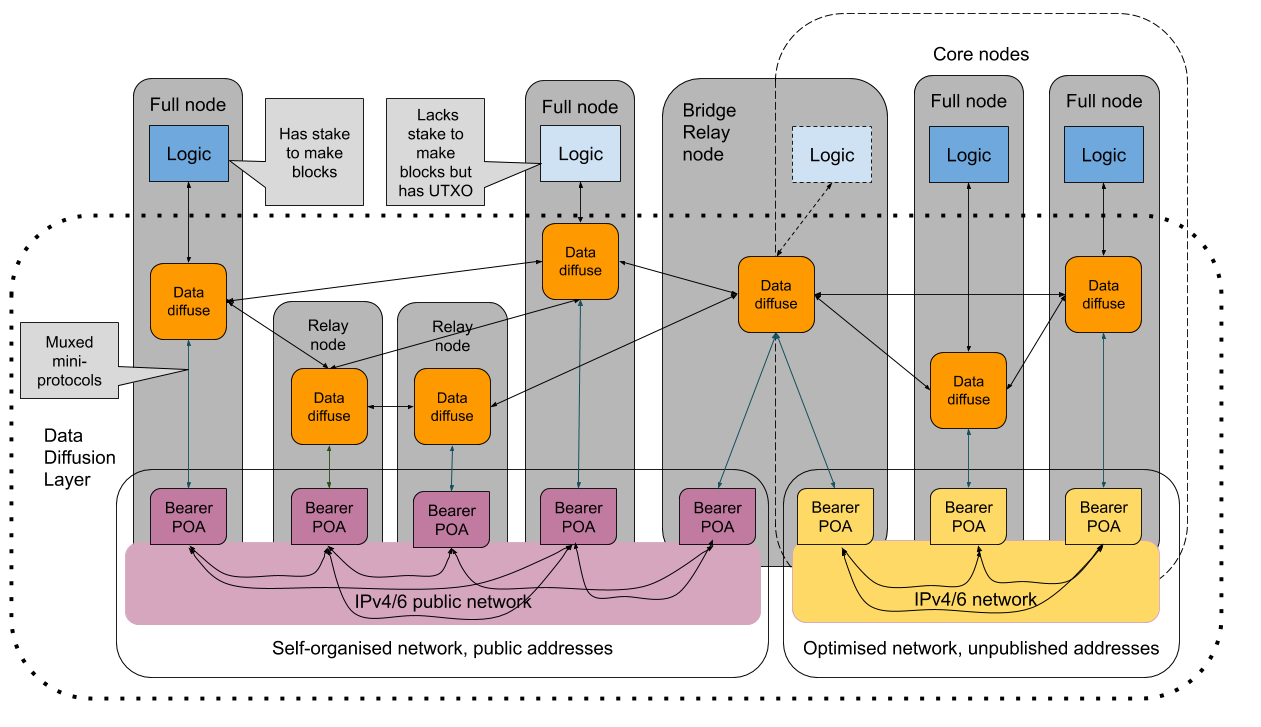
\includegraphics[width=6.26772in,height=3.61111in]{./media/image5.png}

\subsection{Development approach}
\label{development-approach}

To deal with the threat of an adversary who knows the code (which is
inevitable for an open-source project), two methods were used to
eliminate implementation errors:

\begin{enumerate}
\def\labelenumi{\arabic{enumi}.}
\item
  \begin{quote}
  Make maximum use of the Haskell type system;
  \end{quote}

  \begin{enumerate}
  \def\labelenumii{\alph{enumii}.}
  \item
    \begin{quote}
    Using a simple version of session types\footnote{Session types:
      \href{https://groups.inf.ed.ac.uk/abcd/}{{https://groups.inf.ed.ac.uk/abcd/}}};
    \end{quote}
  \end{enumerate}
\item
  \begin{quote}
  Build on the idea of an executable specification by being able to run
  the actual code in a simulated mode, which enables;
  \end{quote}

  \begin{enumerate}
  \def\labelenumii{\alph{enumii}.}
  \setcounter{enumii}{1}
  \item
    \begin{quote}
    control over entropy and timing for reproducibility;
    \end{quote}
  \item
    \begin{quote}
    regression testing;
    \end{quote}
  \item
    \begin{quote}
    trying out worst-case scenarios.
    \end{quote}
  \end{enumerate}
\end{enumerate}

\subsubsection{Session Type Framework}
\label{session-type-framework}

An important feature of any protocol design is avoiding deadlock, in
which both parties are either waiting for something or trying to send
something to the other at the same time. The solution in Shelley is
agency management, in which exactly one peer has agency at any time,
enforced by the Haskell type system. This approach avoids deadlock while
allowing pipelining, which overcomes the effect of bearer latency on
performance-critical protocols. Pipelining can be implemented without
changing protocol description or the server implementation -- only the
client side of the code has to be altered.

This is achieved using a Session Type framework, in which protocols are
described as state machines encoded into Haskell types. The
implementations that engage in these typed protocols are required to
respect the protocol description, and this is enforced by the types. The
state machine descriptions are constrained so that in each protocol
state only one peer may send, while the other must receive. This
guarantees that the protocols are free from race conditions or
deadlocks. This eliminates a class of bugs and makes testing
significantly easier.

The session type framework was also developed to allow the construction
of polymorphic protocols: protocols which can be instantiated with
different concrete data, e.g. the developed chain sync protocol is
independent of the block type\footnote{It is also similarly independent
  of the codec (transformation between concrete and abstract syntax).}
which allows it to be used for different ouroboros protocols like
Ouroboros-BFT or Ouroboros-Praos. Applying types to protocols rather
than channels allows the channels to be polymorphic, so that there is no
need to create a separate channel for each protocol.\\
~\\
The session type framework has been tremendously helpful in the design
phase of each mini-protocol. It allowed us to communicate and discuss
concise ideas, both within our own team and to other teams (e.g. the
Wallet team). This is similar to the way other teams are using
mathematical notation to precisely formulate and communicate ideas. The
difference is that we used the strong type system of Haskell to encode
protocols with mathematical precision, providing proofs of their
correctness. We can also write tests for the protocols without running
them on a network or using multiple threads.

\subsection{Point-to-point bearers}
\label{point-to-point-bearers}

The idea is to use a single `bearer' between peers over which all
interactions are multiplexed . This allows us to control the resources
that can be consumed at a node by any connected peer, thereby minimising
the scope for resource consumption attacks, including peer-related
denial-of-service attacks. This has the downside of making the RTT more
of a problem for performance, which we manage with pipelining (see
\cref{performance}). We apply backpressure to
manage edge conditions, while minimising head-of-line blocking
effects\footnote{Failure to clear the queues by reading from the TCP
  socket will cause the receive window to fill up and the sender will
  stop sending more data. No data is lost and no packets are
  retransmitted, but no progress is made.} by means of explicit
multiplexing on the bearer. This gives us control over precedence of
delivery and the emergent properties of the bearer by having the point
of contention within the local node's domain of control.

The abstract notion\footnote{Following the principle of
  compositionality,} of a `bearer' carrying a single ordered stream
allows a range of connectivity types to be accommodated, from local
sockets to satellite links. Although the initial wide-area bearer will
be TCP, this generic approach means that other interprocess
communication mechanisms can be used. For example communication between
different processes (e.g. wallet backend) and the node can be done
entirely within the security confines of a single machine.

This also accords with the `minimise resource usage' principle expressed
at the start of §6, by using only one TCP port per connected peer. Also,
using a uniform abstraction reduces the attack surface.

\subsection{Demand-driven spanning tree}
\label{demand-driven-spanning-tree}

The set of nodes that blocks need to reach quickly is given by the stake
distribution/number of stake pools. The block distribution time then
depends on the topology of the peer interconnections between these
nodes. As discussed in
\cref{decentralisation-constraints}, Cardano nodes
can detect eclipse attacks, unlike PoW systems such as Bitcoin, and so
the Kademlia approach of enforcing randomness on the connectivity graph
to make such attacks more difficult is not required. A more pressing
requirement for Cardano is to limit the number of hops blocks must
traverse\footnote{So that the per-node hop time target is achievable for
  a globally distributed system: this is discussed in more detail in the
  Annex.}, and so the decision was taken to use a demand-driven spanning
tree approach, in which each node makes independent choices of which of
its peers to download new data from. Each node maintains a local list of
peers, divided into three sets:

\begin{longtable}[]{@{}ll@{}}
\toprule
\textbf{State} & \textbf{Definition}\tabularnewline
\midrule
\endhead
Cold & A `cold' peer is one which the node is aware of but has not yet
connected with\tabularnewline
Warm & A `warm' peer is one that the node has established a bearer
connection with, and is following its chain, but is not currently using
to obtain new blocks or transactions\tabularnewline
Hot & A `hot' peer is one that the node is actively using to obtain
blocks and/or transactions\tabularnewline
\bottomrule
\end{longtable}

Peers delivering data that is incorrect or late are rapidly deselected,
i.e. removed or demoted from `hot' to `warm'. The `cold' set is
populated at start-up (as described in
\cref{decentralisation-design}) and refreshed by
lists of addresses provided on connection with peers. A node will move
peers between these sets in response to receiving (or not) the number of
well-formed blocks that it expects. Ultimately, if this fails (which
could indicate a possible eclipse attack) it will have to return to its
bootstrap procedure to obtain new `cold' peers.

While it is important to minimise block propagation time, it is also
important to avoid forming cliques (strongly-connected subgraphs)
because this creates the risk that the network could be partitioned by
the loss of only a few bearers. This means some `warm' peers will need
to be `far off' (i.e. kept in the set even if they perform poorly).

As discussed in
\cref{decentralisation-constraints}, one constraint
is the total capacity of the network interface of a node. Each connected
peer that is downloading blocks from the node will consume up to
\textasciitilde{}1Mbit/s. Thus a `domestic' node with a 10Mbit/s uplink
capacity could not accept requests from more than 10 peers. In extreme
cases it might only serve blocks it generated itself!

\subsection{Protocol framework}
\label{protocol-framework}

\subsubsection{Compositionality}
\label{compositionality}

Shelley fundamentally improves on Byron by having a \emph{compositional}
design. This strong form of modularity means that separate aspects of
each protocol's behaviour, resource consumption, and robustness can be
designed and reasoned about independently.

The protocol framework is designed to maximise compositionality by using
independent `mini-protocols' for distinct functions (sidestepping the
typical combinatorial complexity explosion) so that no single protocol
becomes too complex to reason about. Key mini-protocols are:

\begin{itemize}
\item
  \begin{quote}
  Bulk block sync
  \end{quote}
\item
  \begin{quote}
  Chain following -- filter useful interactions to the consensus
  component
  \end{quote}
\item
  \begin{quote}
  Transaction submission
  \end{quote}
\end{itemize}

A separate function called `the Mux' multiplexes these mini-protocols
onto a point-to-point bearer for each connected peer node. This provides
a common approach to version control, managing load and controlling
resource consumption using isometric flow control.

The wireformat used by Mux is simple and compact which gives a low
overhead, both in bytes over the network and in CPU cycles\footnote{Note
  that the efficiency of the encoding is important as it affects the
  network interface capacity required, which in turn constrains who can
  effectively run a Cardano node, as discussed in
  \cref{fundamental-tradeoffs}}.

\subsubsection{Structured information exchanges}
\label{structured-information-exchanges}

A naive implementation of Ouroboros would transmit far more data than
strictly necessary, making it impossible to meet the timeliness
constraint. Thus an important design approach was to analyse the
information exchange requirements (IERs) and then map these onto data
transfers in the most efficient way, while avoiding opening up
opportunities for adversaries to attack the system. This is described
above in
\cref{consensus-constraints-and-design-decisions}

Resulting design decisions include:

\begin{itemize}
\item
  \begin{quote}
  Exchanging blocks rather than broadcasting chains;
  \end{quote}

  \begin{itemize}
  \item
    \begin{quote}
    All practical consensus algorithms do this -- it is simply a
    mathematical convenience to formulate the Ouroboros algorithm in
    terms of broadcasting chains;
    \end{quote}
  \end{itemize}
\item
  \begin{quote}
  Interleaving forwarding with validation
  \end{quote}

  \begin{itemize}
  \item
    \begin{quote}
    To prevent adversaries consuming resources by sending invalid data;
    \end{quote}
  \end{itemize}
\item
  \begin{quote}
  Sending block headers ahead of whole blocks, using the chain-sync
  protocol;
  \end{quote}

  \begin{itemize}
  \item
    \begin{quote}
    this allows a node to decide whether it needs to download a full
    block;
    \end{quote}
  \item
    \begin{quote}
    if it does it can choose which peer to download it from;
    \end{quote}
  \end{itemize}
\item
  \begin{quote}
  Sending transaction IDs ahead of full transactions;
  \end{quote}

  \begin{itemize}
  \item
    \begin{quote}
    Request a number of transactions;
    \end{quote}
  \item
    \begin{quote}
    Receive a set of (short) transaction IDs and sizes;
    \end{quote}
  \item
    \begin{quote}
    Request a subset of those transactions.
    \end{quote}
  \end{itemize}
\end{itemize}

Details of these protocols can be found in the
\href{https://hydra.iohk.io/build/1011577/download/1/network.pdf}{{second
part of the design documentation}}.

\subsubsection{Protocol polymorphism}
\label{protocol-polymorphism}

A key point is the separation of:

\begin{itemize}
\item
  \begin{quote}
  codec
  \end{quote}
\item
  \begin{quote}
  channel, and
  \end{quote}
\item
  \begin{quote}
  consensus logic
  \end{quote}
\end{itemize}

This enables early and thorough testing ahead of the integration of the
parts.

The protocol driver takes the codec as a parameter, which allows for
different choices of encoding. Codecs themselves can also be
polymorphic, for example in the type of blocks or transactions. This
aids in enabling the consensus and network layer combination to be
parameterized by the choice of the ledger rules and representation.
Allowing different choices of ledger rules improves the future
flexibility and enables reuse of these components in other products.

The protocols are also polymorphic in the consensus algorithm, which
provides a clean separation of concerns between the components and
allows consensus algorithm evolution without changing the data diffusion
code.

\subsection{Performance assessment and optimisation}
\label{performance-assessment-and-optimisation}

The strict timeliness constraints of block diffusion means that the data
diffusion component must constantly monitor and optimise performance.
Each node evaluates the performance of its peer connections by measuring
their $\Delta{}Q$ {[}Comp20{]}, at both the bearer and mini-protocol levels. This
enables efficient performance-optimising decisions by the
mini-protocols; for instance, the block-fetch protocol can select
between several different peers offering the same block(s) on the basis
of which would be expected to deliver soonest based on their measured
$\Delta{}Q$.

Congestion between each pair of nodes is managed by the Mux function,
and overall congestion at the network interface of a node is bounded by
\emph{isometric flow-control} (meaning that the potential outstanding
traffic is limited)

The `topography' is the combination of topology and performance.
Performance is a function of both capacity and distance, because
achievable TCP download speeds depend on the round-trip time (RTT) of
the bearer (this is discussed in more detail in \cref{tcp-rpc-response-behavior}).
The goal is to optimise the topography of the data diffusion network,
not just its topology.

\subsection{Summary response to threats}
\label{summary-response-to-threats}

Here we summarise the responses to the threats discussed in
\cref{high-level-threat-model} embodied in the
Shelley network design.

\begin{longtable}[]{@{}ll@{}}
\toprule
\textbf{Threat} & \textbf{Response}\tabularnewline
\midrule
\endhead
Adversarial peers & Detect adversarial behaviour (including poor
performance) and drop the connection to that peer\tabularnewline
Resource exhaustion attacks & Structure protocols so as to strictly
bound the resources that any connected peer can consume (attempting to
consume more than the protocol allows would be adversarial, see row
above)\tabularnewline
Tier-1 actors & Ensure nodes are sufficiently distributed and diverse so
that no single tier-1 actor can isolate a large proportion of the total
stake\tabularnewline
Bearer-level attacks & Design the network architecture so that large
stake-holding nodes are defended against DoS attacks\tabularnewline
\bottomrule
\end{longtable}

\subsection{Bootstrap}
\label{bootstrap}

Note that the problem of NAT/firewalls means that there is no way to
construct a network without at least some nodes having accessible public
IP addresses. A new node joining the network needs to be able to find
these addresses. This can be achieved in different ways, depending on
the deployment scenarios:

\begin{itemize}
\item
  \begin{quote}
  The node can be provided with IP addresses in a configuration file;
  \end{quote}

  \begin{itemize}
  \item
    \begin{quote}
    This would be the default option for an exchange or stakepool node,
    or in an enterprise setting;
    \end{quote}
  \end{itemize}
\item
  \begin{quote}
  The node can be provided with DNS names in a configuration file;
  \end{quote}

  \begin{itemize}
  \item
    \begin{quote}
    This would be the default option for smaller nodes, including
    wallets
    \end{quote}
  \end{itemize}
\end{itemize}

Once a node has succeeded in connecting to one peer, that peer can
provide addresses of other peers that it knows; note that the receiving
node does not need to trust the addresses that it is given, as it can
try them out for itself and make dynamic decisions about which peers it
uses as described in §7.5. This exchange of information about (the
addresses of) other nodes is called `gossiping', and is required for the
fully decentralised version of Shelley (2.2). The implementation that
will be taken here is inspired by Kademlia, but can be far less complex.

\section{Outstanding and unresolved issues}
\label{outstanding-unresolved-issues}

\subsection{Cold/black start scenarios}
\label{coldblack-start-scenarios}

Cold start scenarios arise when some event has taken all block-producing
nodes and other intermediate nodes offline for some time. Examples
include natural disasters such as solar storms, or catastrophic software
or configuration failures.

In such a scenario, restarting the system cannot be achieved by the
network layer alone. These scenarios break the assumptions of Ouroboros
and handling them may require Ouroboros protocol modifications, and may
also require additional out-of-band communication between stake pool
operators. This requires further analysis.

\subsection{Resources and decentralisation}
\label{resources-and-decentralisation}

The size ratio between empty and full blocks is more than 3000, and to
create full blocks a similar amount of data must be moved in
transactions. Thus the minimum amount of data to be received by each
node varies from \textasciitilde{}1kb/20s (system idle) to
\textasciitilde{}2Mb/20s (leaf node) to \textasciitilde{}4Mb/20s (full
node). The amount of data transmitted by a full node will exceed this in
proportion to the number of peers downloading from it.

This creates a risk (which occurs in practice in other industries) that
the capacity of nodes may be dimensioned on the basis of historical
`typical' load (i.e. mostly empty blocks), so that if a burst of large
transactions occurs requiring full-sized blocks to be created, such
nodes will not be able to keep up. If such load is sustained, the
integrity of Cardano might be at risk.

This is an example of a hazard which, although it appears distributed,
has a correlate (and part of potential normal operation) criteria for
arming that hazard, with an associated reputational risk. Although there
are node configuration parameters to contain this problem, their correct
use cannot be enforced once the system is decentralised

There are a number of non-technical risks related to third-party
behaviour in Ouroboros/Cardano related to the operation of stakepools.
Typical industry practice for handling this is to create a certification
/ conformance programme, i.e. tie this into aspects of branding.
Assuring the veracity of stakepool holders claims about the resource
allocation and other stakepool operation is, perhaps, something that the
Cardano Foundation could help manage through a suitable conformance /
certification programme.

\section{Annexes}
\label{annexes}

\subsection{Business requirements}
\label{business-requirements}

The high level business requirements reproduced below were signed
off in late 2017.

They are expressed in informal prose, often following a ``user story''
style. Roughly, there are three kinds of users:

\begin{enumerate}
\def\labelenumi{\arabic{enumi}.}
\item
  \begin{quote}
  users who have delegated,
  \end{quote}
\item
  \begin{quote}
  small stakeholders, and
  \end{quote}
\item
  \begin{quote}
  large stakeholders.
  \end{quote}
\end{enumerate}

\subsubsection{Network connectivity}
\label{network-connectivity}

\paragraph{Participate as a user who has delegated}

As a Daedalus home user with my stake delegated to other users I would
like to join the Cardano network so I can participate in the network.

\begin{enumerate}
\def\labelenumi{\arabic{enumi}.}
\item
  \begin{quote}
  The system must be designed to provide this user segment with the
  ability to catch up and keep up with the blockchain without having to
  do any local network configuration.
  \end{quote}
\item
  \begin{quote}
  The system must be designed to provide this user segment with the
  ability to continuously find and maintain a discovery of a sufficient
  number of other network participants that have reasonable
  connectivity.
  \end{quote}
\item
  \begin{quote}
  The system must be designed to provide this user segment with the
  ability to find and maintain a minimum of 3 other network participants
  to maintain connectivity with performance that is sufficient to catch
  up with the blockchain.
  \end{quote}
\item
  \begin{quote}
  The system design will take into account that this user will probably
  be behind a firewall.
  \end{quote}
\item
  \begin{quote}
  Users in the segment can be defined by having all their stake
  delegated to other network participants. As such they will never be
  selected as a slot leader (i.e required to generate a block).
  \end{quote}
\end{enumerate}

\paragraph{Participate in network as small stakeholder}

As a Daedalus home user operating a node with a small stake, I would
like to join the Cardano network so I can participate in the network as
a node that produces blocks i.e. my stake is not delegated to someone
else.

\begin{enumerate}
\def\labelenumi{\arabic{enumi}.}
\item
  \begin{quote}
  The system must be designed to provide this user segment with the
  ability to receive the transactions that will be incorporated into
  blocks (although sizing the operation of the distributed system to
  ensure that all such participants would be able to receive all
  transactions is not a bounding constraint).
  \end{quote}
\item
  \begin{quote}
  The system must be designed to provide this user segment with the
  ability to participate in the MPC protocol\footnote{Note that this
    requirement is now redundant as the MPC protocol is required only
    for Ouroboros Classic}.
  \end{quote}
\item
  \begin{quote}
  The system will be designed to provide this user segment with the
  ability to catch up and keep up with the blockchain without having to
  do any local network configuration (this is a bounding constraint).
  \end{quote}
\item
  \begin{quote}
  The user will have sufficient connectivity and performance to receive
  a block within a time slot AND they have to be able to create and
  broadcast a block within a time slot in which the block is received by
  other participating nodes.
  \end{quote}
\item
  \begin{quote}
  The system will be designed to maximise the likelihood that 50\% of
  home users operating a participating node are compliant with the
  previous requirement at any one time.
  \end{quote}
\item
  \begin{quote}
  The system will be designed to provide this user segment with the
  ability to continuously find and maintain a discovery of a sufficient
  number of other network participants that have reasonable
  connectivity.
  \end{quote}
\item
  \begin{quote}
  The system will provide a discovery mechanism that will find and
  maintain a minimum of 3 other network participants to maintain
  connectivity with performance that is sufficient to catch up with the
  blockchain.
  \end{quote}
\item
  \begin{quote}
  The system design will take into account that this user may be behind
  a firewall (i.e being behind a firewall should not preclude a user
  participating in this fashion).
  \end{quote}
\item
  \begin{quote}
  The Delegation workstream will provide a UI feature for the user to
  choose to control their own stake.
  \end{quote}
\item
  \begin{quote}
  Users in this segment will be defined as NOT
  \end{quote}

  \begin{enumerate}
  \def\labelenumii{\alph{enumii}.}
  \item
    \begin{quote}
    being in the top 100 users ranked by stake or
    \end{quote}
  \item
    \begin{quote}
    in a ranked set of users who together control 80\% of the stake
    \end{quote}
  \end{enumerate}
\item
  \begin{quote}
  Users in this segment will not be part of the Core Dif, but still
  subject to the normal incentives related to creating blocks.
  \end{quote}
\end{enumerate}

\paragraph{Participate in network as a large stakeholder}
\label{participate-in-network-as-a-large-stakeholder}

As a user running a core node on a server and with large stake in the
network, I would like to join the Cardano network so I can participate
in the network as a core server node that produces blocks i.e. have not
delegated to someone else.

\begin{enumerate}
\def\labelenumi{\arabic{enumi}.}
\item
  \begin{quote}
  A large stakeholder will be defined as
  \end{quote}

  \begin{enumerate}
  \def\labelenumii{\alph{enumii}.}
  \item
    \begin{quote}
    being in the top 100 users ranked by stake; or
    \end{quote}
  \item
    \begin{quote}
    in a ranked set of users who combined control 80\% of the stake
    \end{quote}
  \end{enumerate}
\item
  \begin{quote}
  Assuming that this user has sufficient connectivity and performance,
  the system should ensure that the collective operation of the
  distributed system will ensure that they have a high probability of
  receiving a block within a time slot such that they have sufficient
  time to be able to create and broadcast a block within a time slot
  where the block is received by other core nodes.
  \end{quote}
\item
  \begin{quote}
  It is expected that the previous requirement will be fulfilled to a
  high degree of reliability between nodes in this category -- assuming
  normal network operations
  \end{quote}
\end{enumerate}

\begin{longtable}[]{@{}ll@{}}
\toprule
Threshold & \textgreater{} 95\%\tabularnewline
\midrule
\endhead
Target & \textgreater{} 98\%\tabularnewline
Stretch & \textgreater{} 99\%\tabularnewline
\bottomrule
\end{longtable}

\begin{enumerate}
\def\labelenumi{\arabic{enumi}.}
\setcounter{enumi}{3}
\item
  \begin{quote}
  The system will be designed to provide this user segment with the
  ability to continuously find and maintain a discovery of a sufficient
  number of other network participants that have reasonable
  connectivity.
  \end{quote}
\item
  \begin{quote}
  Discovery will find and maintain a minimum of 10 other network
  participants to maintain connectivity with performance that is
  sufficient to catch up with the blockchain.
  \end{quote}
\item
  \begin{quote}
  Ability to receive the transactions that will be incorporated into
  blocks.
  \end{quote}
\item
  \begin{quote}
  Ability to participate in the MPC protocol\footnote{Note that this
    requirement is now redundant as the MPC protocol is required only
    for Ouroboros Classic}.
  \end{quote}
\item
  \begin{quote}
  The user will catch up and keep up with the blockchain.
  \end{quote}
\item
  \begin{quote}
  The server firewall rules will be such that it can communicate with
  other core nodes on the system (and vice versa) -- The system will
  provide the necessary information to update firewall rules if the
  server is operating behind a firewall to ensure the server can
  communicate with other core nodes.
  \end{quote}
\item
  \begin{quote}
  The threshold which defines the group of large stakeholders may be
  configurable on the network layer. The configuration may include
  toggling between the rules a) and b) in the previous requirement and
  the threshold numbers within these (this is pending a decision from
  the Incentives workstream.
  \end{quote}
\item
  \begin{quote}
  The rules and threshold configuration may need to be a protocol
  parameter that is updated by the update system.
  \end{quote}
\end{enumerate}

\subsubsection{Network performance}
\label{network-performance}

\paragraph{Poor network connectivity notification}

As a home user, I want to see a network connection status on Daedalus so
that I know the state of my network connection.

\begin{itemize}
\item
  \begin{quote}
  If the user receives a notification that they are in red or amber
  mode, Daedalus will give the user some helpful information on how to
  resolve common connectivity issues.
  \end{quote}
\end{itemize}

There are three (at least) the following three distinct modes that the
network can be operating in: each one has a red, green, amber status.

\begin{longtable}[]{@{}ll@{}}
\toprule
Initial block sync &\tabularnewline
\midrule
\endhead
red & receiving \textless{} 1 blocks per 10s\tabularnewline
amber & receiving \textless{} 10 blocks per 10s\tabularnewline
green & otherwise\tabularnewline
Recovery &\tabularnewline
red & receiving \textless{} 1 block per 10s\tabularnewline
amber & otherwise\tabularnewline
green & (not applicable)\tabularnewline
Block chain following &\tabularnewline
red & it has been more than 200s since a slot indication was
received.\tabularnewline
amber & it has been more than 60s since a slot indication was
received.\tabularnewline
green & otherwise.\tabularnewline
\bottomrule
\end{longtable}

This assumes that the slot time remains 20 seconds\footnote{Under Praos
  this should be interpreted as the average time between production of
  new blocks is 20 seconds.}.

\paragraph{Transaction Throughput}

The transaction per second of the system as a whole will be:

\begin{longtable}[]{@{}ll@{}}
\toprule
\emph{Threshold} & 8 tps\tabularnewline
\midrule
\endhead
\emph{Target} & 16 tps\tabularnewline
\emph{Stretch} & 50 tps\tabularnewline
\bottomrule
\end{longtable}

This assumes that the slot time remains 20 seconds.

\paragraph{Network Bearer Resource Use -- end user control}

As a user operating on the network as a home user not behind a firewall,
I would like a cap on the total amount of network capacity in terms of
short-term bandwidth that other network users can request from my
connection so I am assured my network resource is not eaten up by the
data diffusion function.

\begin{enumerate}
\def\labelenumi{\arabic{enumi}.}
\item
  \begin{quote}
  The cap should be based on a fraction of a typical home internet
  connection -- it can be changed by configuration including ``don't act
  as a super node''.
  \end{quote}
\item
  \begin{quote}
  The system will allow users syncing with the latest version of the
  blockchain to download blocks from more then one and up to five
  network peers concurrently.
  \end{quote}
\item
  \begin{quote}
  A cap on the number of incoming subscribers.
  \end{quote}
\item
  \begin{quote}
  A cap on number of outbound requests for block syncing from other
  users.
  \end{quote}
\item
  \begin{quote}
  The cap will not be imposed on core nodes running on a server.
  \end{quote}
\item
  \begin{quote}
  If these resources are available, a reasonable connection speed should
  be available to users requesting to sync the latest version of the
  blockchain e.g. downloading blocks from 5 peers concurrently to
  aggregate the bandwidth.
  \end{quote}
\item
  \begin{quote}
  (nice to have) the actual number and capacity being used is available
  to users.
  \end{quote}
\end{enumerate}

\paragraph{Participant performance measurement}

There may be a requirement for measuring if a large stakeholder is not
meeting their network obligation Br\"unjes et al. (2018).

It is accepted that this requirement is a ``nice to have'', and it has
not been established that it is possible, nor has it been incorporated
into the incentives mechanism.

\subsubsection{Distributed System Resilience and Security}
\label{distributed-system-resilience-and-security}

\paragraph{Resilience to abuse}

As a user I should not be able to attack the system using an asymmetric
denial of service attack that will deplete network resources from other
users.

\begin{enumerate}
\def\labelenumi{\arabic{enumi}.}
\item
  \begin{quote}
  The system should achieve its connectivity and performance
  requirements even in the presence of a non-trivial proportion of bad
  actors on the network.
  \end{quote}
\item
  \begin{quote}
  There is an assumption that there are not large numbers of bad actors
  in the network.
  \end{quote}
\item
  \begin{quote}
  The previous assumption does not follow from the assumptions of
  Ouroboros which states that the users that control 50\% of the stake
  are non-adversarial.
  \end{quote}
\end{enumerate}

\paragraph{DDoS protection}

As a large stakeholder running a core node on a server, I should still
be able to communicate with other users in this segment, even if the
system comes under a DDoS attack.

\begin{itemize}
\item
  \begin{quote}
  Users in this segment will be able to generate and broadcast blocks to
  each other within the usual timing constraints in this situation.
  \end{quote}
\end{itemize}

IP addresses will be hidden.

\begin{itemize}
\item
  \begin{quote}
  Encrypted IP addresses will be published by 10 of the other members of
  the group of large stakeholder core nodes.
  \end{quote}
\end{itemize}

Assumption

\begin{itemize}
\item
  \begin{quote}
  Core node operators will not publish their IP addresses publicly.
  \end{quote}
\item
  \begin{quote}
  Encrypted IP addresses will be published by the 10 of the other
  members of the group of large stakeholder core nodes.
  \end{quote}
\item
  \begin{quote}
  If a node operator's IP address is compromised the operator will
  respond and change the IP address of their node.
  \end{quote}
\item
  \begin{quote}
  The system will allow operators to change the address of their core
  nodes and communicate with that new IP address within a reasonable
  period of time.
  \end{quote}
\end{itemize}

\subsubsection{Network decentralisation}
\label{network-decentralisation}

\paragraph{No hegemony}

As a user I want to be assured that IOHK and its business partners are
not in an especially privileged position in terms of trust,
responsibility and necessity to the network so that network hegemony is
avoided.

\begin{itemize}
\item
  \begin{quote}
  IOHK should be in the same position on the network as any other
  stakeholder with an equivalent amount of stake.
  \end{quote}
\item
  \begin{quote}
  There is a more general requirement that no other actor could achieve
  hegemonic control of the operation of the data diffusion layer.
  \end{quote}
\end{itemize}

\subsection{TCP RPC response behavior}
\label{tcp-rpc-response-behavior}

In Shelley we are using (pre-established) TCP/IP bearers, over which
information exchanges are multiplexed.

\begin{enumerate}
\def\labelenumi{\arabic{enumi}.}
\item
  \begin{quote}
  Given the interval between block diffusions we are assuming that the
  TCP/IP congestion window will be reset to its \emph{IW} (initial
  window)\footnote{See §4.1 in
    \href{https://tools.ietf.org/html/rfc5681}{{https://tools.ietf.org/html/rfc5681}}
    -- the reset to initial conditions timer is based on the TCP
    retransmit timer (see
    \href{https://tools.ietf.org/html/rfc6298}{{https://tools.ietf.org/html/rfc6298}}
    §2). For Cardano deployments within AWS this has a credible upper
    bound of one second (by observation and analysis), even between the
    most distant locations.}.
  \end{quote}
\item
  \begin{quote}
  There is a plethora of options for TCP/IP window scaling
  algorithms\footnote{See
    \href{https://en.wikipedia.org/wiki/TCP_congestion_control}{{https://en.wikipedia.org/wiki/TCP\_congestion\_control}}
    -- it should be noted that this work has as its goal throughput
    fairness under saturation of a common resource with long lived data
    flows, whereas our data flows are relatively short. Other flow
    control mechanisms that are not available in a TCP/IP environment,
    such as rate-based, may be more suitable for our needs.}, but
  changing them on a particular machine requires superuser access, which
  violates the constraint in §6.
  \end{quote}
\item
  \begin{quote}
  As our exemplar environment here we are considering AWS linux
  deployments, specifically contemporary AWS Ubuntu images.
  \end{quote}
\end{enumerate}

\subsubsection{Time to transmit a block of given size across given latencies}
\label{time-to-transmit-a-block-of-given-size-across-given-latencies}

The $\Delta{}Q|_G$ value\footnote{The concept of $\Delta{}Q$ is
  explained in {[}Comp20{]}. Here is a link to
  \href{https://www.slideshare.net/pnsol-slides/q-and-blockchain-83943683}{{slides
  on applicability to block chain}}.} here is for the round trip time,
the $\Delta{}Q|_S$ is 8\texttimes{}10\textsuperscript{-8} s/o (the
typical value from tests), and the $\Delta{}Q$ per direction is taken to be ½ the
round trip (reasonable in an AWS environment, not so in an asymmetric
networking case e.g. residential, SME)

Note that window size is always restricted in practice: the unrestricted
window case is presented here to capture the causality restriction
within the slow-start TCP paradigm.

The tables show the time in seconds to achieve the bulk transfer (as per
the outcome description above) -- their likely accuracy is ± 1 RTT (left
hand column) due to various vagaries of how actual behaviour is context
sensitive. Note that this does not model the initial request time, but
also note that the IW size can be 10, which reduces RTT count by one or
so, so these effects are cancelled out for longer transfers as the
actual ``bandwidth-delay product'' dominates those (i.e. once the TCP
window is fully open). The red `danger' colour shows block transfer
times that risk missing the targets set in §6.1.

\begin{longtable}[]{@{}lllllllllll@{}}
\toprule
Unrestricted Window Size & & & & & & & & & &\tabularnewline
\midrule
\endhead
& File size (kb) & & & & & & & & &\tabularnewline
$\Delta{}Q|_G$ (s) & 2 & 5 & 10 & 20 & 50 & 100 & 200 &
500 & 1000 & 2000\tabularnewline
0.002 & 0.001 & 0.001 & 0.003 & 0.005 & 0.007 & 0.010 & 0.012 & 0.017 &
0.025 & 0.042\tabularnewline
0.005 & 0.003 & 0.003 & 0.008 & 0.013 & 0.018 & 0.023 & 0.028 & 0.035 &
0.044 & 0.061\tabularnewline
0.010 & 0.005 & 0.005 & 0.015 & 0.025 & 0.035 & 0.046 & 0.056 & 0.068 &
0.080 & 0.097\tabularnewline
0.020 & 0.010 & 0.010 & 0.030 & 0.050 & 0.070 & 0.091 & 0.111 & 0.133 &
0.155 & 0.180\tabularnewline
0.050 & 0.025 & 0.025 & 0.075 & 0.125 & 0.175 & 0.226 & 0.276 & 0.328 &
0.380 & 0.435\tabularnewline
0.100 & 0.050 & 0.050 & 0.150 & 0.250 & 0.350 & 0.451 & 0.551 & 0.653 &
0.755 & 0.860\tabularnewline
0.150 & 0.075 & 0.075 & 0.225 & 0.375 & 0.525 & 0.676 & 0.826 & 0.978 &
1.130 & 1.285\tabularnewline
0.200 & 0.100 & 0.100 & 0.300 & 0.500 & 0.700 & 0.901 & 1.101 & 1.303 &
1.505 & 1.710\tabularnewline
0.250 & 0.125 & 0.125 & 0.375 & 0.625 & 0.875 & 1.126 & 1.376 & 1.628 &
1.880 & 2.135\tabularnewline
0.300 & 0.150 & 0.150 & 0.450 & 0.750 & 1.050 & 1.351 & 1.651 & 1.953 &
2.255 & 2.560\tabularnewline
\bottomrule
\end{longtable}

The next table represents the ``best credible case'' (between AWS
instances before kernel parameters have to be changed) for a large
window size that can be set from within a user program.

\begin{longtable}[]{@{}lllllllllll@{}}
\toprule
Large max window size (near default maximum) & & & & & & & & &
&\tabularnewline
\midrule
\endhead
& File Size (ko) & & & & & & & & &\tabularnewline
$\Delta{}Q|_G$ (s) & 2 & 5 & 10 & 20 & 50 & 100 & 200 &
500 & 1000 & 2000\tabularnewline
0.002 & 0.001 & 0.001 & 0.003 & 0.005 & 0.007 & 0.010 & 0.012 & 0.017 &
0.025 & 0.042\tabularnewline
0.005 & 0.003 & 0.003 & 0.008 & 0.013 & 0.018 & 0.023 & 0.028 & 0.035 &
0.044 & 0.062\tabularnewline
0.010 & 0.005 & 0.005 & 0.015 & 0.025 & 0.035 & 0.046 & 0.056 & 0.068 &
0.087 & 0.119\tabularnewline
0.020 & 0.010 & 0.010 & 0.030 & 0.050 & 0.070 & 0.091 & 0.111 & 0.133 &
0.172 & 0.234\tabularnewline
0.050 & 0.025 & 0.025 & 0.075 & 0.125 & 0.175 & 0.226 & 0.276 & 0.328 &
0.427 & 0.579\tabularnewline
0.100 & 0.050 & 0.050 & 0.150 & 0.250 & 0.350 & 0.451 & 0.551 & 0.653 &
0.852 & 1.154\tabularnewline
0.150 & 0.075 & 0.075 & 0.225 & 0.375 & 0.525 & 0.676 & 0.826 & 0.978 &
1.277 & 1.729\tabularnewline
0.200 & 0.100 & 0.100 & 0.300 & 0.500 & 0.700 & 0.901 & 1.101 & 1.303 &
1.702 & 2.304\tabularnewline
0.250 & 0.125 & 0.125 & 0.375 & 0.625 & 0.875 & 1.126 & 1.376 & 1.628 &
2.127 & 2.879\tabularnewline
0.300 & 0.150 & 0.150 & 0.450 & 0.750 & 1.050 & 1.351 & 1.651 & 1.953 &
2.552 & 3.454\tabularnewline
\bottomrule
\end{longtable}

Note a $\Delta{}Q|_{G,S}$ of (300ms, 8\texttimes{}10\textsuperscript{-8} o/s) is not the
absolute worst case -- the worst we've measured (in other work) is
$\Delta{}Q|_{G,S}$ of (188ms, 6.14\texttimes{}10\textsuperscript{-5} o/s) \emph{one-way}
between San Paulo and Singapore. This would give a time-to-complete of
5.38s in the 2000 ko transfer case.

The next table represents the default case -- i.e. no special action on
the code and hence acceptance of the contemporary window size default.

\begin{longtable}[]{@{}lllllllllll@{}}
\toprule
Medium max window size (near default) & & & & & & & & & &\tabularnewline
\midrule
\endhead
& File Size (ko) & & & & & & & & &\tabularnewline
$\Delta{}Q|_{G,S}$  (s) & 2 & 5 & 10 & 20 & 50 & 100 & 200 &
500 & 1000 & 2000\tabularnewline
0.002 & 0.001 & 0.001 & 0.003 & 0.005 & 0.007 & 0.010 & 0.012 & 0.017 &
0.025 & 0.042\tabularnewline
0.005 & 0.003 & 0.003 & 0.008 & 0.013 & 0.018 & 0.023 & 0.028 & 0.039 &
0.055 & 0.090\tabularnewline
0.010 & 0.005 & 0.005 & 0.015 & 0.025 & 0.035 & 0.046 & 0.056 & 0.076 &
0.107 & 0.178\tabularnewline
0.020 & 0.010 & 0.010 & 0.030 & 0.050 & 0.070 & 0.091 & 0.111 & 0.151 &
0.212 & 0.353\tabularnewline
0.050 & 0.025 & 0.025 & 0.075 & 0.125 & 0.175 & 0.226 & 0.276 & 0.376 &
0.527 & 0.878\tabularnewline
0.100 & 0.050 & 0.050 & 0.150 & 0.250 & 0.350 & 0.451 & 0.551 & 0.751 &
1.052 & 1.753\tabularnewline
0.150 & 0.075 & 0.075 & 0.225 & 0.375 & 0.525 & 0.676 & 0.826 & 1.126 &
1.577 & 2.628\tabularnewline
0.200 & 0.100 & 0.100 & 0.300 & 0.500 & 0.700 & 0.901 & 1.101 & 1.501 &
2.102 & 3.503\tabularnewline
0.250 & 0.125 & 0.125 & 0.375 & 0.625 & 0.875 & 1.126 & 1.376 & 1.876 &
2.627 & 4.378\tabularnewline
0.300 & 0.150 & 0.150 & 0.450 & 0.750 & 1.050 & 1.351 & 1.651 & 2.251 &
3.152 & 5.253\tabularnewline
\bottomrule
\end{longtable}

\subsubsection{Examples of TCP/IP window opening between London and Sydney}
\label{examples-of-tcpip-window-opening-between-london-and-sydney}

The figure below shows the window size over a four-minute run:

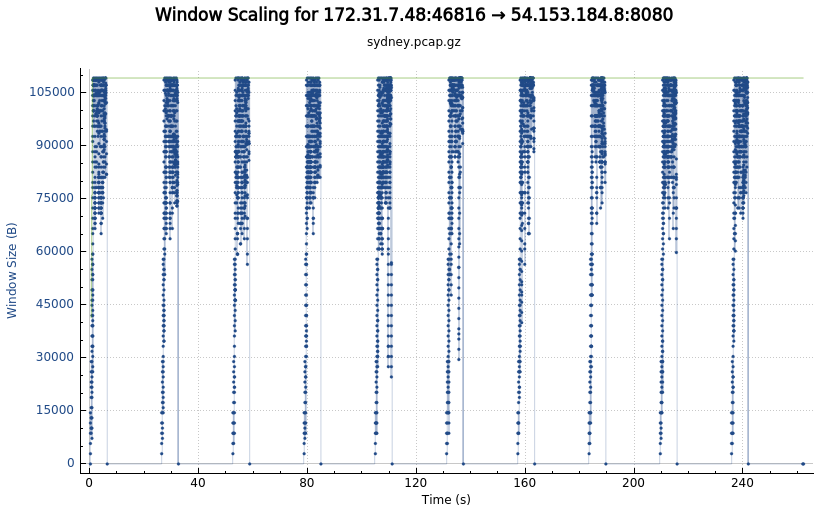
\includegraphics[width=6.27083in,height=3.88889in]{./media/image1.png}

The following figure shows the contemporaneous round trip (as reported
from TCP):

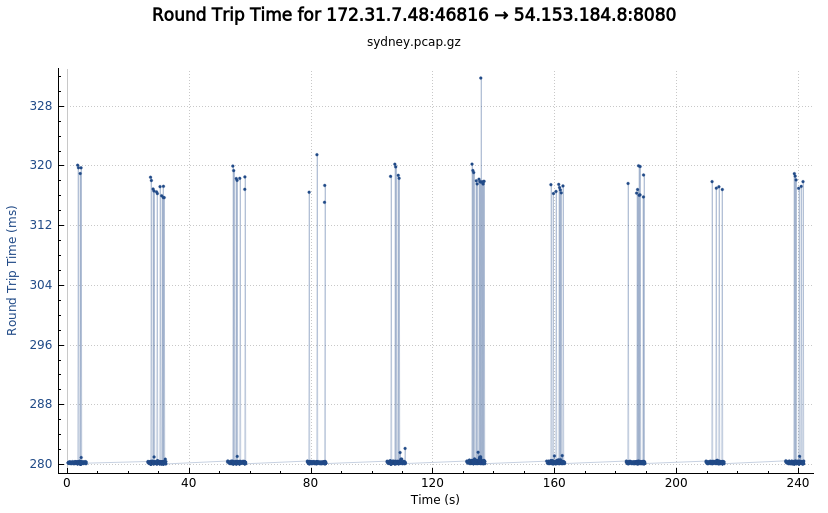
\includegraphics[width=6.27083in,height=3.88889in]{./media/image4.png}

Note that the outliers in round trip time are (most likely) relating to
those packets that were at the end of the round trip time / window
closing -- most ACKs would have been triggered by the ``two packet
rule''; if an odd number of packets arrived just before a pause, its
acknowledgement would be dependent on the ACK timeout
(\textasciitilde{}40ms ?).

\subsection{Model of network scaling}
\label{model-of-network-scaling}

Per-hop budget for ``data diffusion''

\begin{longtable}[]{@{}llll@{}}
\toprule
& Threshold & Target & Stretch\tabularnewline
\midrule
\endhead
\textbf{Max hops} & \textbf{20s budget} & \textbf{15s budget} &
\textbf{10s budget}\tabularnewline
2 & 10.0s & 7.5s & 5.0s\tabularnewline
3 & 6.6s & 5.0s & 3.3s\tabularnewline
4 & 5.0s & 3.75s & 2.5s\tabularnewline
5 & 4.0s & 3.0s & 2.0s\tabularnewline
\bottomrule
\end{longtable}

These budgets should be compared with the time-to-complete for
delivering a block in \cref{time-to-transmit-a-block-of-given-size-across-given-latencies}.

Size of spanning tree as a function of depth and node valency (assuming
homogeneity):

\begin{longtable}[]{@{}llllll@{}}
\toprule
& Valency & & & &\tabularnewline
\midrule
\endhead
Depth & 2 & 3 & 4 & 5 & 6\tabularnewline
2 & 7 & 26 & 63 & 124 & 215\tabularnewline
3 & 15 & 80 & \emph{\textbf{255}} & \emph{\textbf{624}} &
1295\tabularnewline
4 & 31 & 242 & \emph{\textbf{1023}} & \emph{\textbf{3124}} &
7775\tabularnewline
5 & 63 & 728 & \emph{\textbf{4095}} & \emph{\textbf{15624}} &
46655\tabularnewline
6 & 127 & 2186 & 16383 & 78124 & 279935\tabularnewline
\bottomrule
\end{longtable}

The shading represents increasing `success' in reaching a large number
of nodes. However, as discussed in §6.2, a large depth is problematic
because it reduces the per-hop time budget, and a large valency is
problematic because it increases the resources required by a node. The
figures in red represent reasonable compromises.

\subsection{Performance model of Ouroboros Praos}
\label{performance-model-of-ouroboros-praos}

\begin{longtable}[]{@{}lll@{}}
\toprule
\textbf{Parameter} & \textbf{Description} &
\textbf{Notes}\tabularnewline
\midrule
\endhead
N & Number of active nodes & Expected to be
\textasciitilde{}1000\tabularnewline
T\textsubscript{s} & Duration of a slot & Expected to be
\textasciitilde{} 2s\tabularnewline
f & Active slot fraction & $0 < f \leq 1$\tabularnewline
$\Delta$ & Maximum number of slots before a diffused message is received & $\Delta \geq 1$\tabularnewline
k & Depth of chain for effective immutability &\tabularnewline
\bottomrule
\end{longtable}

\subsubsection{Distribution of leadership}
\label{distribution-of-leadership}

From {[}BGKR17{]}, the probability of stakeholder U\textsubscript{i}
with relative stake \(\alpha_{i}\)being chosen in any slot is:

\(p_{i} = {\phi_{f}\left( \alpha_{i} \right) = 1 - \left( 1 - f \right)^{\alpha_{i}}}_{}\)

We assume here that each of the N active nodes has an equal amount of
stake\footnote{The incentive system is designed to encourage a uniform
  distribution of stake between major nodes.},
\(\alpha_{i} = \frac{1}{N}\), and hence equal probability of being a
leader in any particular slot. Then:

\(p_{i}{= 1 - \left( 1 - f \right)^{\frac{1}{N}}}_{}\)

The probability that stakeholder Ui is not the leader is
\({1 - p}_{i} = \left( 1 - f \right)^{\frac{1}{N}}\), and so the
probability that no stakeholder is the leader (i.e. we have an empty
slot) is\footnote{Each node decides independently whether it is the
  leader, so we just multiply probabilities.}:

\(P\left( \text{no\ leader} \right) = \left( \left( 1 - f \right)^{\frac{1}{N}} \right)^{N} = \ 1 - f\)

(Hence the definition of f as the active slot fraction). If the
probability of leadership was directly proportional to stake it would be
\(\frac{f}{N}\) for each node. The error relative to the true function
above is:

\({E_{f,N} = p}_{i} - \frac{f}{N} = 1 - \frac{f}{N} - \left( 1 - f \right)^{\frac{1}{N}} \simeq 1 - \frac{f}{N} - \left( 1 - \frac{f}{N} + {\frac{\left( \frac{1}{N} - 1 \right)}{2N}f}^{2} \right) \simeq \frac{f^{2}}{2N}\)

For reasonably large N and small f we could ignore this error term, and
use the linear approximation\footnote{Which is simpler than the true
  Binomial distribution.}. This would imply:

\(P\left( \text{one\ leader} \right) = f\left( 1 - \frac{f}{N} \right)^{N - 1}\)

In the large N limit\footnote{The intention is to encourage
  \textasciitilde{}1000 stake pools, which is enough for the large N
  limit to be quite accurate.} this becomes:

\(P\left( \text{one\ leader} \right) = fe^{- f}\)

Conversely, the probability of a run of m successive empty slots (since
these are independent trials) is:

\(P_{m}^{\text{NL}} \equiv P(m\ slots\ no\ leader)\  = {P(no\ leader)}^{m} = \left( 1 - f \right)^{m}\)

This gives the following table:

\begin{longtable}[]{@{}lllllllllll@{}}
\toprule
& \textbf{Active slots fraction \emph{f}} & & & & & & & &
&\tabularnewline
\midrule
\endhead
m & 0.1 & 0.2 & 0.3 & 0.4 & 0.5 & 0.6 & 0.7 & 0.8 & 0.9 &
1\tabularnewline
1 & 9.00E-01 & 8.00E-01 & 7.00E-01 & 6.00E-01 & 5.00E-01 & 4.00E-01 &
3.00E-01 & 2.00E-01 & 1.00E-01 & 0.00E+00\tabularnewline
3 & 7.29E-01 & 5.12E-01 & 3.43E-01 & 2.16E-01 & 1.25E-01 & 6.40E-02 &
2.70E-02 & 8.00E-03 & 1.00E-03 & 0.00E+00\tabularnewline
10 & 3.49E-01 & 1.07E-01 & 2.82E-02 & 6.05E-03 & 9.77E-04 & 1.05E-04 &
5.90E-06 & 1.02E-07 & 1.00E-10 & 0.00E+00\tabularnewline
31 & 3.82E-02 & 9.90E-04 & 1.58E-05 & 1.33E-07 & 4.66E-10 & 4.61E-13 &
6.18E-17 & 2.15E-22 & 1.00E-31 & 0.00E+00\tabularnewline
100 & 2.66E-05 & 2.04E-10 & 3.23E-16 & 6.53E-23 & 7.89E-31 & 1.61E-40 &
5.15E-53 & 1.27E-70 & 1.00E-100 & 0.00E+00\tabularnewline
\bottomrule
\end{longtable}

We can convert slots into a time interval by multiplying by Ts.
Conversely, if we want to know the probability that a certain time
interval t will be leaderless, we can approximate this\footnote{Ignoring
  the quantisation of m.} as:

\(P_{t}^{\text{NL}} \equiv P(t\ seconds\ no\ leader)\  = {P(slot\ has\ no\ leader)}^{\frac{t}{T_{s}}} = \left( 1 - f \right)^{\frac{t}{T_{s}}} = \left( \left( 1 - f \right)^{\frac{1}{T_{s}}} \right)^{t}\)

If we set a threshold Y (say 0.999) for the probability of having at
least one leader in time t, then t is bounded by:

\(t \geq T_{s}\frac{\log\left( 1 - Y \right)}{\log\left( 1 - f \right)}\)

This is relevant for the consideration of timeouts that might be
triggered by a leaderless interval.

\subsection{Comparison with general overlay networks}
\label{comparison-with-general-overlay-networks}

One approach to building a large-scale decentralized blockchain
applications is to take existing P2P protocols designed for other
applications domains (notably P2P file sharing) and use them as the
distributed application infrastructure to build the blockchain itself.
It is a temptingly fast approach, but it comes with a number of
security, scalability and performance hazards:

\begin{enumerate}
\def\labelenumi{\arabic{enumi}.}
\item
  \begin{quote}
  Protocols that were designed for a specific environment (e.g.
  efficient location of distributed content) are not well-suited to the
  requirements of a blockchain. For example, the adoption of the
  Kademlia protocol in Ethereum facilitates low-resource Eclipse attacks
  on the nodes of the blockchain {[}MHG15{]}.
  \end{quote}
\item
  \begin{quote}
  Protocols in a P2P framework are usually designed for a single
  environment, integrated into their original application, and hard to
  repurpose to different requirements. This exercise usually requires a
  redesign and re-implementation of the protocol from scratch, since the
  protocol is not designed with adaptability in mind {[}S19{]}
  \end{quote}
\item
  \begin{quote}
  P2P frameworks mostly focus on the construction and maintenance of the
  overlay structure and on routing application requests / disseminating
  information. Other aspects that are also important for the
  communication of application instances are usually not covered, such
  as:
  \end{quote}

  \begin{itemize}
  \item
    \begin{quote}
    Quality of service: ability to handle multiple classes of
    application traffic within the overlay and differentially allocate
    loss and delay to them.
    \end{quote}
  \item
    \begin{quote}
    Security: authentication, access control, confidentiality and
    message integrity, usually achieved through protocols that are not
    part of the P2P framework such as TLS or DTLS.
    \end{quote}
  \item
    \begin{quote}
    Ability to operate over multiple IP networks (e.g. public Internet
    or private IP networks) or other non-IP bearers (e.g. directly over
    Ethernet).
    \end{quote}
  \end{itemize}
\item
  \begin{quote}
  Scalability of the overlay is achieved ad-hoc. Some P2P frameworks
  introduce the concept of ``super-peers'' {[}M15{]}, but there is no
  formal means of creating hierarchies within the overlay framework.
  \end{quote}
\item
  \begin{quote}
  It is hard to reason about the correctness of a group of
  independently-designed protocols working in conjunction. The
  properties of their joint operation in production environments are
  going to be emergent and hence hard or impossible to control by
  design. The system is always going to be suboptimal from an
  efficiency, security and performance standpoint compared to a solution
  that designs the complete ``communications middleware'' in a coherent
  and integrated fashion.
  \end{quote}
\end{enumerate}

A piecemeal approach to addressing these communication challenges will
not deliver a robust and sustainable solution. In the same way that
following a typical industry `low assurance' approach to software
development risks sinking effort into constantly debugging
poorly-specified code, continuing with a `business as usual' approach to
network issues risks creating a complex and fragile solution that
similarly consumes an ever-increasing fraction of the available
development and maintenance resources. Instead, we need a consistent
framework in which to define and describe issues and posit and refine
solutions without piling up complexity and technical debt.

\begin{longtable}[]{@{}ll@{}}
\toprule
Feature & Standard P2P overlay framework\tabularnewline
\midrule
\endhead
\textbf{Authentication, access control, confidentiality, integrity} &
Such functions are usually not part of the overlay framework, which
relies on protocols such as TLS and/or DTLS.\tabularnewline
\textbf{Routing and forwarding} & Most literature on P2P overlay
frameworks is about efficient location of distributed content,
leveraging DHT (Distributed Hash Table) technology to achieve consistent
access this goal {[}M15{]}\tabularnewline
\textbf{Support for multihoming} & Rely on limited definition of
multihoming (load balancing only) provided by IP-based technologies
(e.g. multipath TCP or SCTP) or implement specialized
protocols\tabularnewline
\textbf{Support for node mobility (e.g. wallet nodes)} & Relies on home
and foreign agents, tunnels, anchors, and specialized protocols to
construct and maintain the overlay connectivity graph, which are
use-case specific {[}MA13{]}\tabularnewline
\textbf{Efficient operation over heterogeneous physical media (e.g.
fibre, satellite, cellular, WiFi, etc.)} & Would require development of
a specialized transport protocol within the overlay with support for
congestion management. Interconnection with other IP systems dependent
on widespread adoption / specialist gateways. Not addressed by P2P
overlay frameworks\tabularnewline
\textbf{Support for QoS (traffic differentiation, routing)} & Multiple
techniques and algorithms available in the literature {[}RS14{]}, but
these are hard (that is, not achieved end-to-end in practice after
\textasciitilde{}50 years since first proposed) to integrate into a
coherent solution\tabularnewline
\textbf{Extensibility / adaptability} & Protocols designed for a single
purpose, need to be redesigned for different environments
{[}S19{]}\tabularnewline
\textbf{Efficiency of the system specification and implementation} &
Each ``control protocol'' specifies its own encoding format, information
modelling and dissemination mechanisms.\tabularnewline
\textbf{Structured / generic approach towards scalability} & No, ad-hoc
extensions (e.g. ``super-peers'' {[}M15{]})\tabularnewline
\textbf{Support for non-IP bearers?} & No, designed to be overlaid on
top of IP networks\tabularnewline
\textbf{Collaborative management of the overlay} & Hard to manage a
group of independently designed protocols working in conjunction: lack
of commonality and of a consistent theory of operation\tabularnewline
\bottomrule
\end{longtable}

\subsection{Time synchronisation constraints}
\label{time-synchronisation-constraints}

Ouroboros Praos (in common with the original `classic' version) assumes
that the notion of a time-slot is unambiguous, which requires
participating nodes to have adequately synchronised local clocks. The
assumption is made in {[}BGKR17{]} that ``any discrepancies between
parties' local clocks are insignificant in comparison with the length of
time represented by a slot''. Since in reality there will be skew
between the local clocks of participating nodes, this implicitly places
a lower limit on the slot time T\textsubscript{s}, and potentially opens
a new attack vector in which an adversary manipulates the time reference
of honest parties.

The current implementation approach is to rely on the NTP service
maintained by OS kernels. This has a number of performance and security
constraints; security concerns are in principle mitigated by the
`secure' variant of the protocol, but few servers support this due to
the computational cost of the cryptographic operations required. In
terms of performance, there is little reliable research, but the
consensus is (from {[}Mills12{]}):

\begin{quote}
As a rule of thumb, the accuracy over the Internet is proportional to
the propagation delay. For a lightly loaded 100-Mb/s Ethernet, the
accuracy is in the order of 100 μs. For an intercontinental Internet
path, the accuracy can be up to several tens of milliseconds.

On network paths with large asymmetric propagation delays, such as when
one direction is via satellite and the other via landline, the errors
can reach 100 ms or more. There is no way these errors can be avoided,
unless there is prior knowledge of the path characteristics.
\end{quote}

Taking 100ms as the credible worst-case, if we interpret `insignificant'
as \textless{} 5\%, this means the minimum slot time T\textsubscript{s}
should not be less than 20 x 100ms = 2s, unless steps are taken to
mitigate sources of NTP inaccuracy. Further research is advisable into
the consequences of violating the clock-synchronisation assumption of
{[}BGKR17{]}, since Cardano is otherwise potentially vulnerable to
NTP-spoofing attacks.

\subsubsection{Leap seconds}
\label{leap-seconds}

A further complication arises from the occasional insertion of `leap
seconds' into UTC. A leap second is a one-second adjustment that is
occasionally applied to civil time Coordinated Universal Time (UTC) to
keep it close to the mean solar time at Greenwich, in spite of the
Earth's rotation slowdown and irregularities. UTC was introduced on
January 1, 1972, initially with a 10 second lag behind International
Atomic Time (TAI). Since that date, 27 leap seconds have been inserted,
the most recent on December 31, 2016 at 23:59:60 UTC, so in 2018, UTC
lags behind TAI by an offset of 37 seconds. When it occurs, a positive
leap second is inserted between second 23:59:59 of a chosen UTC calendar
date and second 00:00:00 of the following date. The definition of UTC
states that the last day of December and June are preferred, with the
last day of March or September as second preference, and the last day of
any other month as third preference. All leap seconds (as of 2017) have
been scheduled for either June 30 or December 31.

Leap seconds do not pose a problem to Praos by themselves; however, the
widespread ambivalence towards them and varied/patchy implementation of
them does. Not all clocks implement leap seconds in the same manner as
UTC {[}RFC7164{]}: leap seconds in Unix time are commonly implemented by
repeating the last second of the day; Network Time Protocol freezes time
during the leap second; other schemes such as those deployed by Google
and Amazon in their public cloud infrastructure smear the lengths of
seconds in the vicinity of a leap second. It would thus be prudent to
avoid generating blocks in the immediate vicinity of a leap second, but
this would require knowing when this is going to happen. Although the
decision about insertion of a leap second is made a long time in
advance, most time distribution systems (SNTP, IRIG-B, PTP) only
announce leap seconds at most 12 hours in advance and sometimes only in
the last minute.

It seems that at worst one validly-generated block may be rejected by
other nodes depending on a temporary time difference, which represents a
level of `adversarial' behavior that Praos can easily withstand.
However, inconsistent implementations of leap second insertion make the
problem much worse. For example, the NTP packet includes a leap second
flag, which informs the user that a leap second is imminent. It has been
reported {[}Malone16{]} that never, since the monitoring began in 2008
and whether or not a leap second should be inserted, have all NTP
servers correctly set their flags on a potential leap second day. This
is one reason many NTP servers broadcast the wrong time for up to a day
after a leap second insertion. Detailed studies of the leap seconds of
2015 and 2016 show that, even for the Stratum-1 servers which anchor the
NTP server network, errors both in leap second flags and the server
clocks themselves are widespread, and can be severe {[}CV18{]}.

Thus, even with all Cardano nodes using NTP, local variations in the
propagation of a leap second could result in persistent differences in
local clock values over many slot times. This clearly violates the
assumption in the Praos paper that differences between local clocks are
insignificant; deeper analysis would be required to understand the
consequences of this to normal operation and what opportunities it
represents for an adversary.

Another problem is that different time standards do not recognise the
accumulation of leap seconds. International Atomic Time (TAI) is exactly
37 seconds ahead of UTC (the 37 seconds results from the initial
difference of 10 seconds at the start of 1972, plus 27 leap seconds in
UTC since 1972). GPS time remains at a constant offset with TAI (TAI −
GPS = 19 seconds), and hence at a constant offset with UTC, although
this offset changes whenever a leap-second is introduced. If a Cardano
node happened to be synchronised with GPS time, say, and failed to
account for the offset to UTC, it would be unable to participate
properly in the protocol.

\subsection{Ouroboros Network Components}
\label{ouroboros-network-components}

The \textbf{Ouroboros Network} implementation consists of the following
Haskell packages:

\begin{enumerate}
\def\labelenumi{\arabic{enumi}.}
\item
  \begin{quote}
  \textbf{typed-protocols} -- a standalone session type framework, which
  allows communication protocols to be expressed and enforced;
  \end{quote}
\item
  \begin{quote}
  \textbf{typed-protocols-cbor} -- a small extension to provide codec
  support for the CBOR format;
  \end{quote}
\item
  \begin{quote}
  \textbf{network-mux} -- a standalone multiplexing library;
  \end{quote}
\item
  \begin{quote}
  \textbf{ouroboros-network-framework} -- a library which makes low
  level choice for \emph{ouroboros-network} and implements low level
  network components / primitives, e.g. connection manager, server.
  \end{quote}
\item
  \begin{quote}
  \textbf{ouroboros-network} -- a library which implements the consensus
  application-level protocols to support \emph{node-to-node} as well as
  \emph{node-to-client} communication (each consists of a bundle of
  \emph{mini-protocols} expressed with \emph{typed-protocols} package),
  and all the required architecture to run them.
  \end{quote}
\end{enumerate}

For the larger picture how all the network components fit together with
the consensus components in a full node, see the diagram in
\cref{consensus-components}.

All the \emph{node-to-node} mini-protocols (\emph{chain-sync},
\emph{block-fetch} and \emph{tx-submission} protocols) are multiplexed
over a single bearer (e.g. TCP socket) using a network-mux package. For
a \emph{node-to-node} (similarly for \emph{node-to-client} protocol) the
networking components are schematically aligned in the following stack:

The bearer is an abstraction which allows reading / writing bytes from
the underlying network (TCP socket, Unix socket, Windows named pipes,
etc.). Protocols are expressed using the session type framework.

\subsubsection{Typed Protocols}
\label{typed-protocols}

Typed protocols is a standalone library which implements a form of
\textbf{session types}. It allows expression of both a server and a
client which stay dual to each other (i.e. being in the same state, and
only one side having the agency to send a message) throughout the
evolution of the protocol. In particular this also means that one cannot
have a deadlock (when two nodes are waiting for the next message), or
being in different states (which would result in receiving an unexpected
message). This library is novel in that it allows the addition of
pipelining, which gives good performance through latency hiding. This
library gives us a way to write protocols in which correctness is proven
by the compiler and still can provide necessary performance
characteristics.. Session types have been a main research topic at some
of the best academic centers, and we received interest from well-known
scientists in the field (prof. Philip Wadler) as well as from the
Haskell community during various events where the framework was
presented\footnote{The framework was presented by Duncan Coutts at
  \href{https://skillsmatter.com/skillscasts/14633-45-minute-talk-by-duncan-coutts}{{Haskell
  eXchange 2019}} , and Marcin Szamotulski at
  \href{https://www.youtube.com/watch?v=j8gza2L61nM}{{Monadic Party
  2019}}.}.

The only prerequisite for using \emph{typed-protocols} is to use bearers
that guarantee order of delivery. Currently, we target TCP, but there
are possible extensions of UDP that could satisfy this constraint, using
other low level network protocols is also plausible. Within a local
computational context we can use named pipes as the bearers, which
removes a lot of complexity.

\subsubsection{Network-Mux}
\label{network-mux}

\emph{network-mux} is a general multiplexing library which allows us to
run multiple protocols over a single bearer. The multiplexer avoids
head-of-line blocking, guarantees fairness and is designed to use
minimal resources.

On the egress end (outbound messages) mini-protocols are competing for a
common resource. The important part of the technical design is to impose
fair share of the resource. In this context we define (and guarantee)
fairness defined as:

\begin{itemize}
\item
  \begin{quote}
  no starvation;
  \end{quote}
\item
  \begin{quote}
  when presented with equal demand (from a selection of mini protocols)
  deliver equal service.
  \end{quote}
\end{itemize}

\emph{network-mux} is designed to support full-duplex bearer
capabilities. This means it can run initiator / responder (client /
server) parts of a mini-protocol at both ends of the connection
simultaneously.

This component is independent of typed-protocols (or any protocol
library), and thus can be used for many different purposes.

\paragraph{Data Flow in Network-Mux}

\subparagraph{Incoming Data path (Ingress path)}

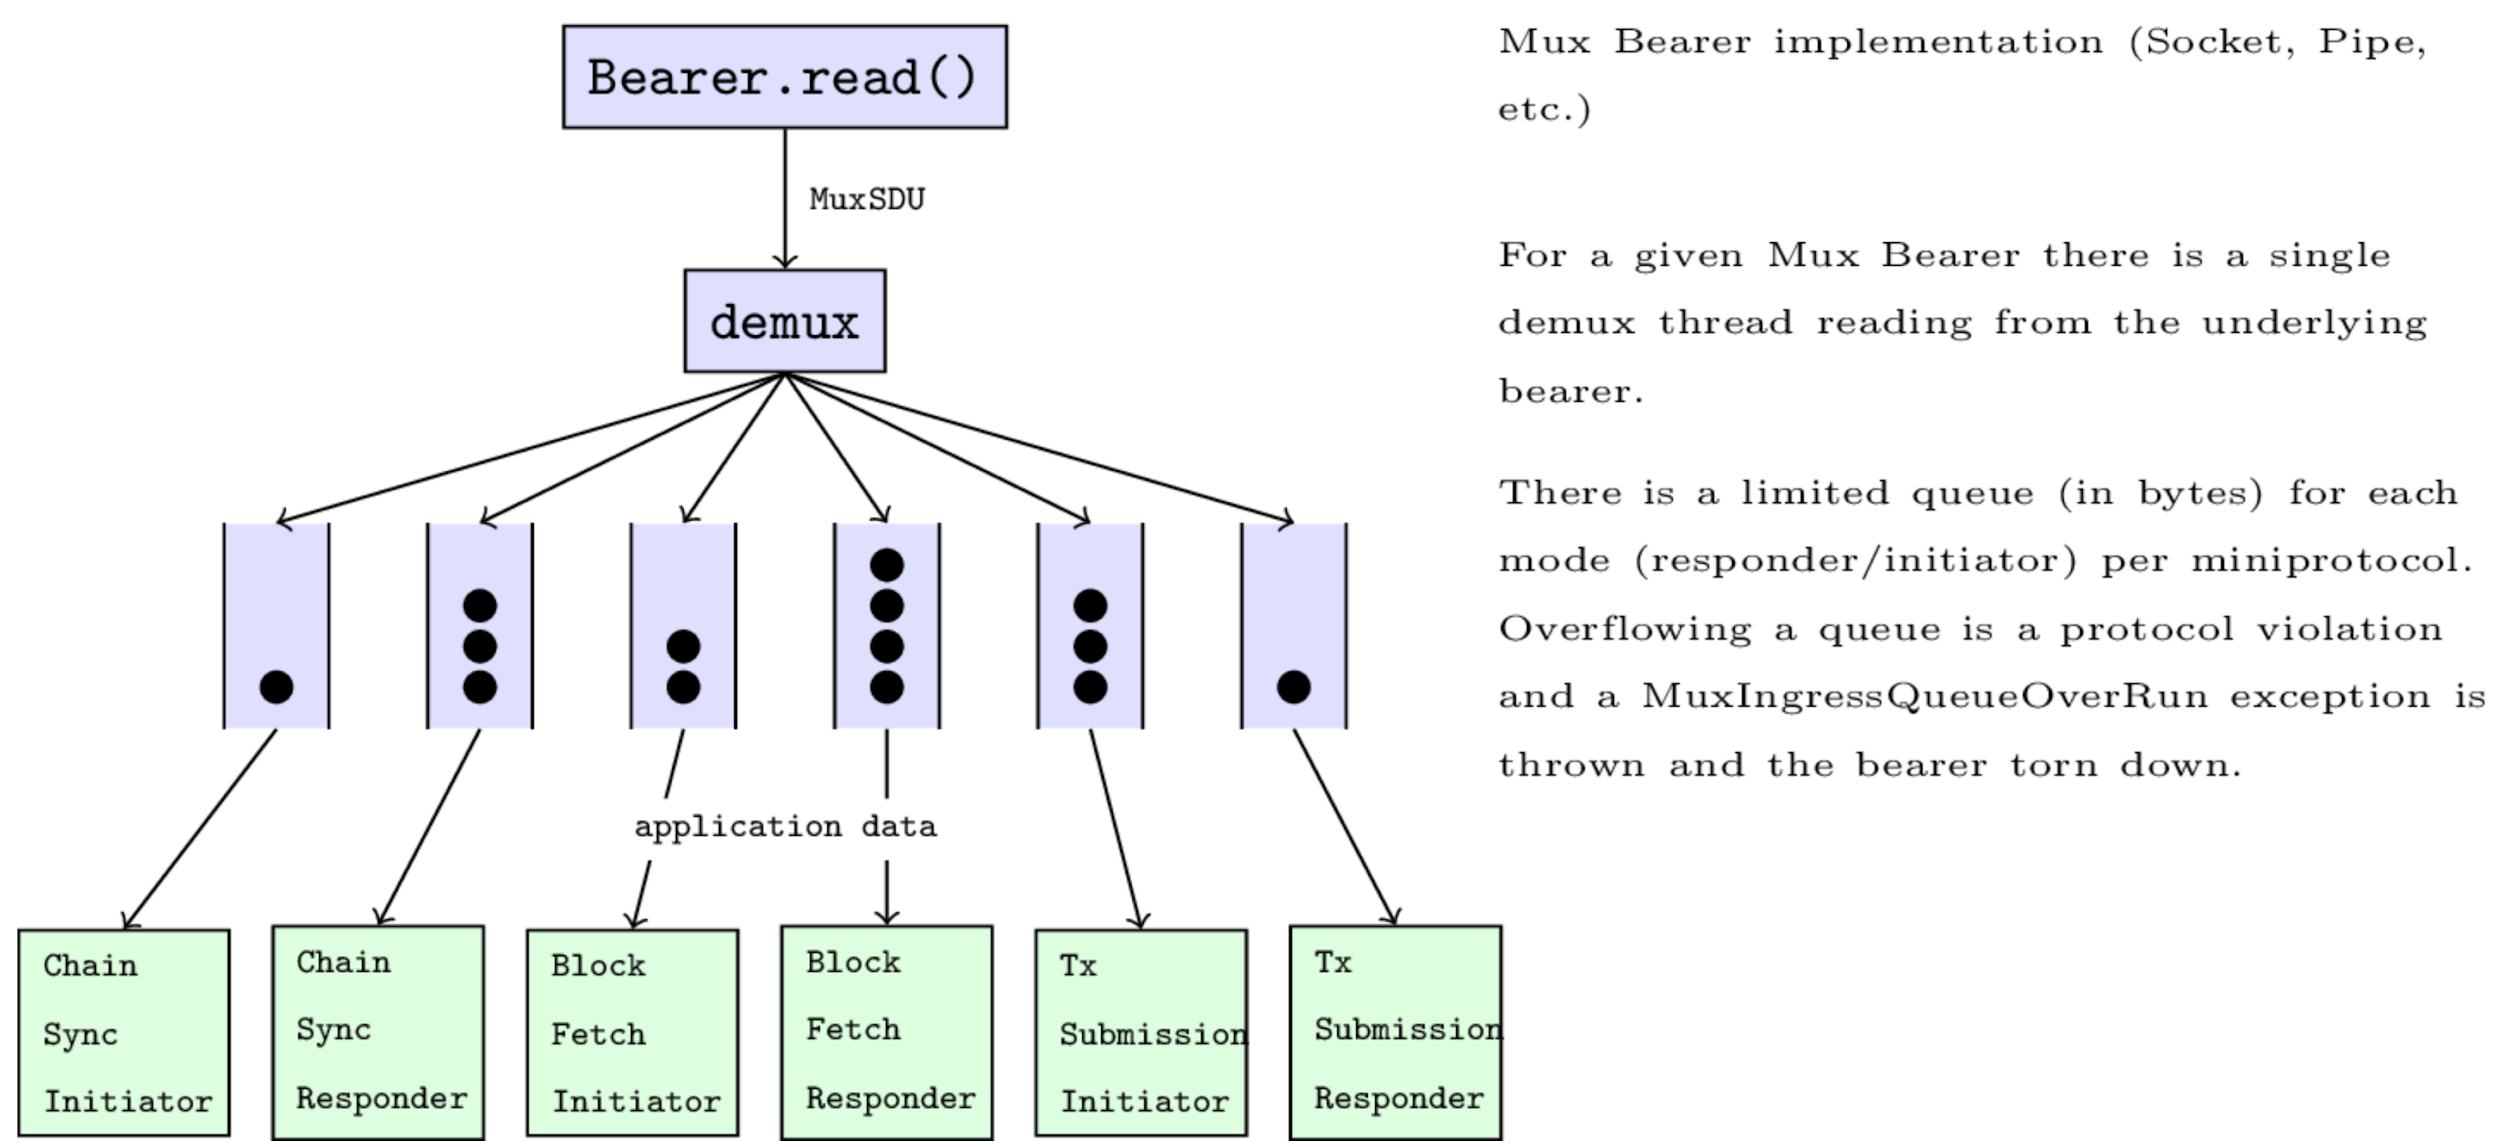
\includegraphics[width=6.27083in,height=2.875in]{./media/image2.png}

\subparagraph{Outgoing Data Path (Egress Path)}

~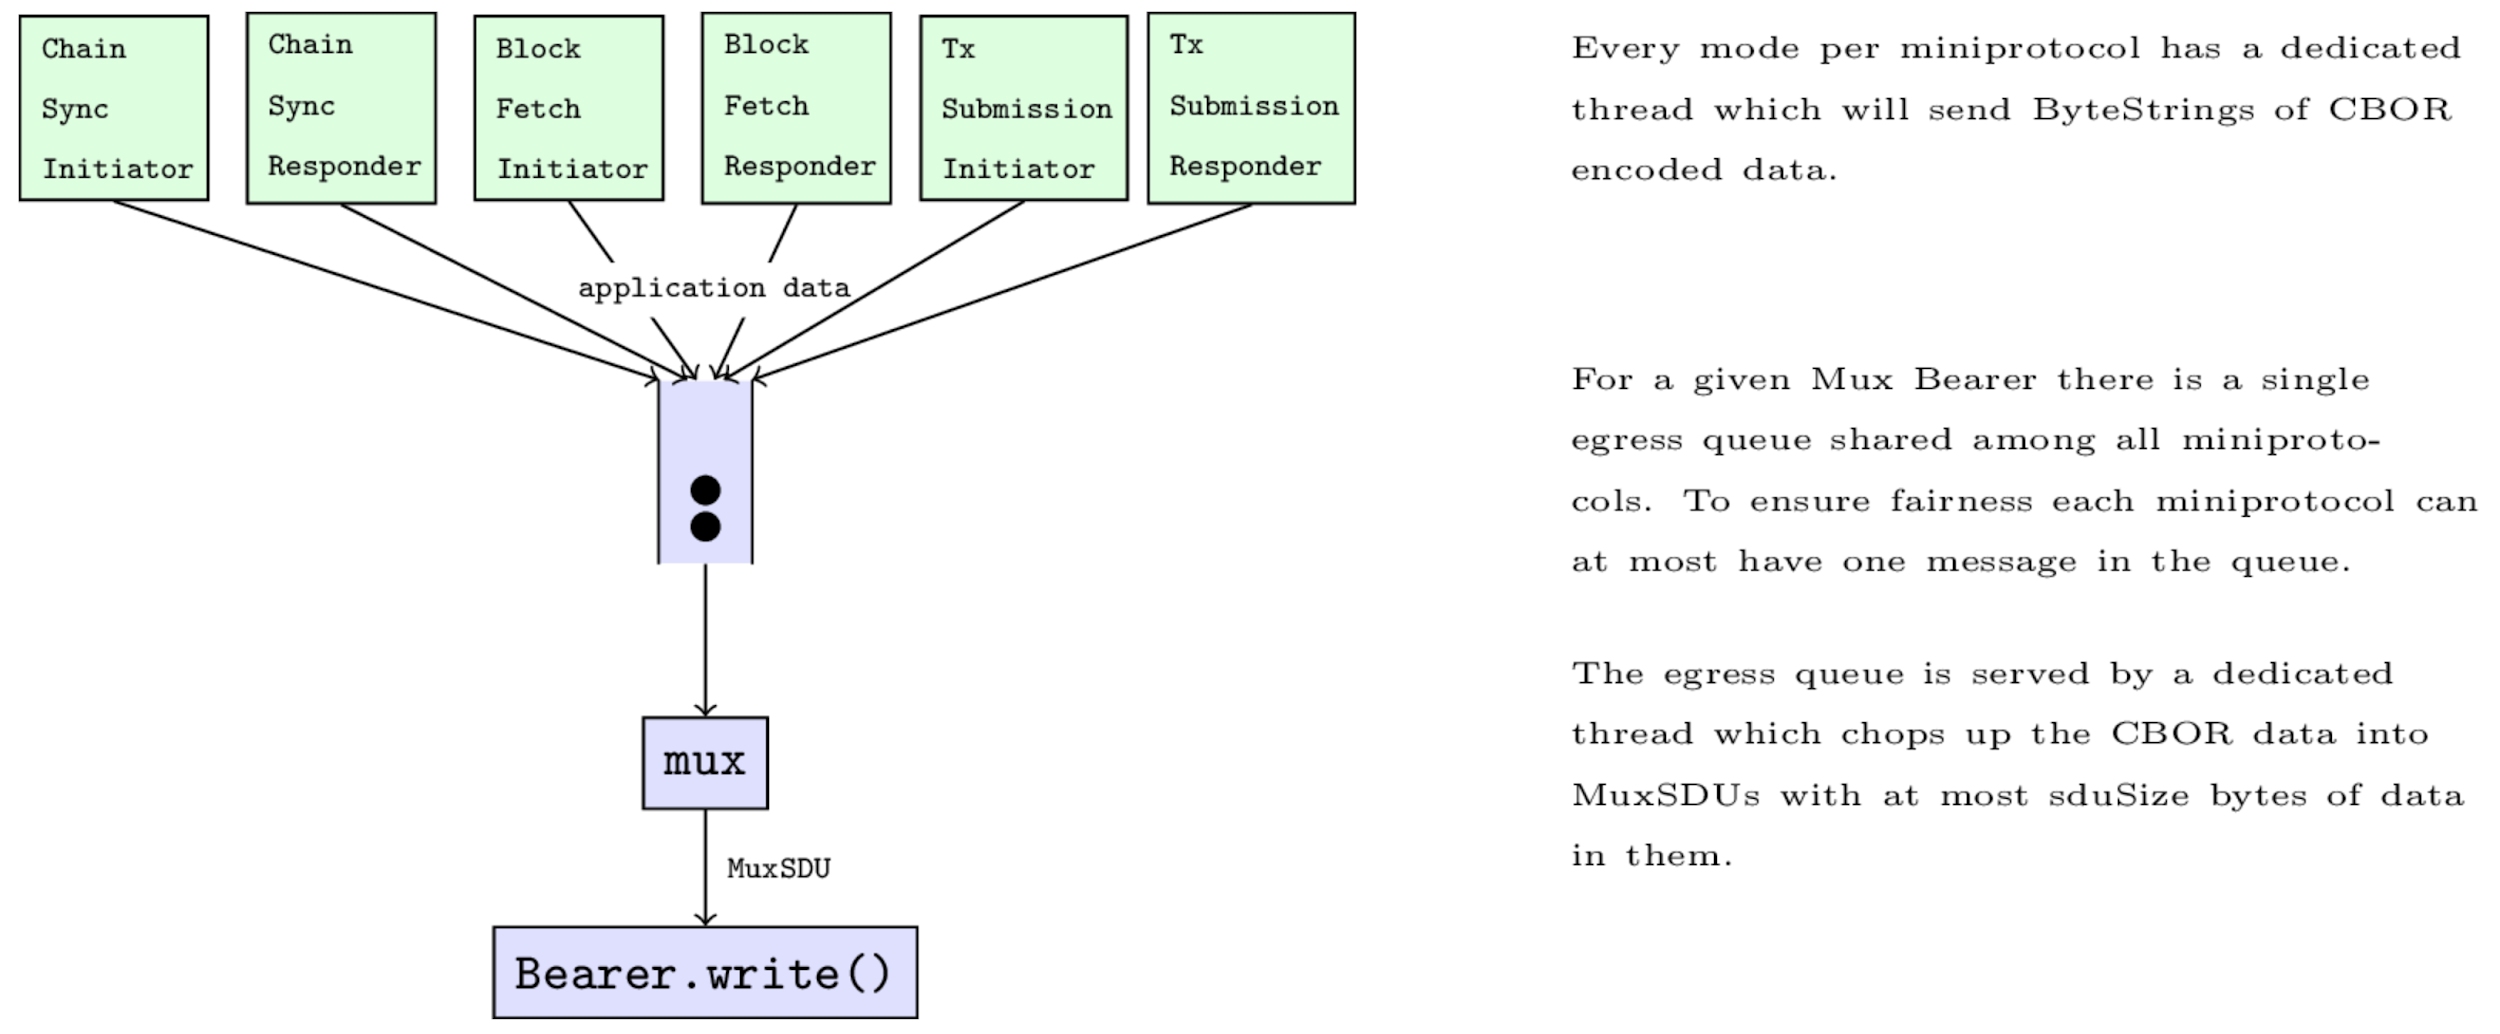
\includegraphics[width=6.27083in,height=2.59722in]{./media/image6.png}

\subsubsection{Ouroboros-Network}
\label{ouroboros-network}

The \emph{ouroboros-network} library implements \textbf{mini-protocols}
for \emph{node-to-node} and \emph{node-to-client} communication using
the typed-protocols package; it provides the means to run them over TCP
sockets, unix sockets, Windows named pipes and can be easily extended to
unix pipes. It also exports an API for writing nodes and clients.

A \emph{node-to-node} protocol consists of:

\begin{itemize}
\item
  \begin{quote}
  \textbf{chain-sync} mini-protocol -- a protocol which allows a node to
  reconstruct a chain of an upstream node;
  \end{quote}
\item
  \begin{quote}
  \textbf{block-fetch} mini-protocol -- a protocol which allows a node
  to download block bodies from various peers;
  \end{quote}
\item
  \begin{quote}
  \textbf{tx-submission} mini-protocol -- a protocol which allows
  submission of transactions.
  \end{quote}
\end{itemize}

A client is a standalone local application which communicates with a
node using a unix-socket (or named-pipe on Windows). This avoids the
design flaw in the Byron era, which is using tcp-sockets and thus needs
to use tls. This has been a source of frustration for many end-users).
Example local clients are: wallets, explorers, command line tools for
various third-parties (e.g. exchanges).

The \emph{node-to-client} protocol consists of:

\begin{itemize}
\item
  \begin{quote}
  \textbf{chain-sync} mini-protocol
  \end{quote}
\item
  \begin{quote}
  \textbf{local-tx-submission} mini-protocol
  \end{quote}
\item
  \begin{quote}
  \textbf{local-state-query} mini-protocol
  \end{quote}
\end{itemize}

From the networking perspective it is not important which flavour of
Ouroboros protocol is being used, and all the protocols reflect that
(the current Haskell implementation is using polymorphism to achieve
this goal). Both \emph{node-to-client} and \emph{node-to-node} protocols
are using the same \emph{chain-sync} protocol, but the difference is
that for the former we are only sending headers through the network,
while the latter is sending whole blocks.

\paragraph{Block Fetch Component}

Block fetch logic is the component responsible for downloading blocks
from connected peers. It runs the client and server sides of the block
fetch protocol, block fetch state per peer and a block fetch logic
component which orchestrates all the downloads. The block fetch logic
makes decisions from whom to download a block (as blocks may be
available from various peers).

\paragraph{Handshake Mini Protocol}

On all incoming connections, before starting the multiplexer we run a
handshake protocol. It allows agreement on protocol parameters. It is
designed so that the whole mini-protocol conversation fits into a single
round trip (at the TCP level).

Currently, in version `V1` we only support network magic, which supports
distinguishing various networks, e.g. stage-net, test-net, main-net. The
protocol is extensible in the sense that any future version can support
its own set of protocol parameters.

\paragraph{Other components of Ouroboros-Network package}

We implemented a peer-to-peer governor which role is to drive decisions
about promotions, demotions and gossip. It is there to provide the rest
of the system with possible peers to communicate with and govern their
state (hot peer / worm peer / cold peer). We are implementing a
connection manager which will manage active connections and threads and
will provide low level primitives which are to be used by the
peer-to-peer governor. The peer-to-peer governor is flexible enough to
handle various deployment scenarios as well as internal usage - we plan
to use it not only in a decentralised setting but also to subscribe
clients (wallets, explorers) over a local bearer to a node.

\subparagraph{Chain Fragments}
\label{chain-fragments}

This is a small part of the Ouroboros-Network package which implements
efficient chain data structure: `ChainFragment` and `AnchoredChain`.
They are hidden at the bottom of the stack since they are useful in
`BlockFetch` component and in various \emph{Ouroboros-Network} tests.

The implementation represents the sequence of headers using a
\href{http://www.staff.city.ac.uk/~ross/papers/FingerTree.html}{finger
tree} data structure instantiated for block headers to enable efficient
O(log n) operations based on slot numbers and block numbers, in addition
to the normal efficient sequence operations.

\subsubsection{Simulator environment SimM}
\label{simulator-environment-simm}

\emph{Source Lines of Code:\\
}

\begin{longtable}[]{@{}lll@{}}
\toprule
\emph{Component} & \emph{sloc} & \emph{sloc of tests}\tabularnewline
\midrule
\endhead
\emph{io-sim-classes} & \emph{\textbf{1148}} & -\tabularnewline
\emph{io-sim} & \emph{\textbf{822}} & \emph{\textbf{601}}\tabularnewline
\bottomrule
\end{longtable}

We wrote a simulation environment for the \emph{IO} monad (which is
called \emph{SimM} or \emph{sim-io}). This is similar to the system that
was used to test the Bitcoin backbone protocol is {[}MJ15{]}. This,
unlike the other components, is very Haskell-specific, and thus its
description below will use language which might be more familiar for
Haskell developers. It is a pure monad (in the same sense as the
\emph{Identity} functor or \emph{Free} monad from the \emph{free}
package). The simulator monad supports the following interfaces:

\begin{itemize}
\item
  \begin{quote}
  software transactional memory \emph{STM}
  \end{quote}
\item
  \begin{quote}
  concurrency in the form of low level \emph{fork} interface and the
  \emph{async} package
  \end{quote}
\item
  \begin{quote}
  \emph{ST} monad interface
  \end{quote}
\item
  \begin{quote}
  synchronous and asynchronous exception handling
  \end{quote}
\item
  \begin{quote}
  timers \emph{API}
  \end{quote}
\item
  \begin{quote}
  monotonic time
  \end{quote}
\end{itemize}

The interface is presented as a set of type classes; its instances are
written with the following principles:

\begin{itemize}
\item
  \begin{quote}
  the \emph{IO} instances are as close to the \emph{base}, \emph{stm}
  and \emph{async} packages as possible (we have very few places where
  we slightly diverge).
  \end{quote}
\item
  \begin{quote}
  the \emph{Sim} instances are faithful to \emph{IO} instances.
  \end{quote}
\end{itemize}

This allows us to write computations that can be interpreted both in
\emph{IO} and the simulator monad \emph{SimM}.

Currently \emph{SimM} provides a single scheduling policy, but it is
possible to extend it, which would improve assurance for tests expressed
using \emph{SimM} monad.

The time in \emph{SimM} is simulated, which allows running tests that
otherwise would take a very long time to complete. Not surprising this
was very useful for testing networking code, but also turned out to be
very useful testing the \emph{ouroboros-consensus} package maintained by
the consensus team.

The simulator environment allows collection of a trace of a computation
(similar to Haskell's eventlog). This is valuable for constructing
complex property tests of some of the components and it has proven
useful in finding low-level bugs that would be extremely difficult to
diagnose in a running system.

The \emph{stm} interface is more general than that of the \emph{stm}
package. It defines strict and lazy versions of stm mutable variables,
what allows tracing of memory leaks.

The hierarchy of classes is slightly different than that of standard
Haskell packages, and it was designed to help in the reviewing process
(both during development, and for external evaluation). Standard Haskell
instances are also exported.

\subsubsection{Testing Strategies}
\label{testing-strategies}

All the protocols are tested on several different levels:

\begin{itemize}
\item
  \begin{quote}
  the \emph{typed-protocol} level, the tests prove that the
  implementation meets the specification. The \emph{type-protocol}
  package turns test errors into type errors. These tests are carried
  for both non-pipelined and pipelined clients.
  \end{quote}
\item
  \begin{quote}
  The wrapper API for each protocol is tested. This is an un-typed
  version of the previous tests. It assures that the client and server
  types are dual to each other. These tests are carried for both
  non-pipelined and pipelined clients.
  \end{quote}
\item
  \begin{quote}
  Test the protocols using example clients and servers over:
  \end{quote}

  \begin{itemize}
  \item
    \begin{quote}
    a channel (using \emph{STM}'s \emph{TMVar}'s)
    \end{quote}
  \item
    \begin{quote}
    using pipes
    \end{quote}
  \end{itemize}
\end{itemize}

All the tests are done in both the \emph{IO} monad and the \emph{SimM}
monad.

Beside protocol tests we also maintain codecs for each protocol and a
testing architecture for them. The typed protocols package exports
properties which allows us to:

\begin{itemize}
\item
  \begin{quote}
  test that decoding is the right inverse to encoding (e.g. decoding an
  encoded message brings back the original message)
  \end{quote}
\item
  \begin{quote}
  test incremental decoders, which allows guarding against boundary
  errors.
  \end{quote}
\end{itemize}

Some of the tests rely on the \emph{SimM} monad which has extensive
tracing support. This allows checking invariants of the running
component. This also permits us to see the evolution of state maintained
by the component, and trace events that are happening in various testing
scenarios. We use this technique in the \emph{BlockFetch},
\emph{peer-to-peer governor} as well as some other components. In all
cases it allowed us to catch subtle bugs early in the development
process.

\section{References}
\label{references}

{[}MM02{]} Maymounkov P., Mazières D. (2002) Kademlia: A Peer-to-Peer
Information System Based on the XOR Metric. In: Druschel P., Kaashoek
F., Rowstron A. (eds) Peer-to-Peer Systems. IPTPS 2002. Lecture Notes in
Computer Science, vol 2429. Springer, Berlin, Heidelberg

{[}JD08{]} John Day, Patterns in Network Architecture: A Return to
Fundamentals, Prentice Hall 2008 ISBN:0132252422 9780132252423

{[}MHG15{]} Y. Marcus, E. Heilman, S. Goldberg. ``Low-Resource Eclipse
Attacks on Ethereum's Peer-to Peer Network''. 24th USENIX Security
Symposium, 2015.

{[}MJ15{]} Andrew Miller, Rob Jansen, Shadow-Bitcoin: Scalable
Simulation via Direct Execution of Multi-threaded Applications, 8th
Workshop on Cyber Security Experimentation and Test, 2015

{[}BGKR17{]} David Bernado, Peter Gaži, Aggelos Kiayias, Alexander
Russell. Ouroboros Praos: An adaptively-secure, semi-synchronous
proof-of-stake blockchain

{[}BGKRZ19{]} Christian Badertscher, Peter Gaži, Aggelos Kiayias,
Alexander Russell, and Vassilis Zikas. Ouroboros Genesis: Composable
Proof-of-Stake Blockchains with Dynamic Availability

{[}SSVV12{]} Setty, Vinay \& van Steen, Maarten \& Vitenberg, Roman \&
Voulgaris, Spyros. (2012). PolderCast: Fast, Robust, and Scalable
Architecture for P2P Topic-Based Pub/Sub. 7662. 271-291.
10.1007/978-3-642-35170-9\_14.

{[}DW13{]} Christian Decker, Roger Wattenhofer, Information Propagation
in the Bitcoin Network, 2013,
\href{https://tik-old.ee.ethz.ch/file//49318d3f56c1d525aabf7fda78b23fc0/P2P2013_041.pdf}{{https://tik-old.ee.ethz.ch/file//49318d3f56c1d525aabf7fda78b23fc0/P2P2013\_041.pdf}}

{[}VFV17{]} Shaileshh Bojja Venkatakrishnan, Giulia Fanti, Pramod
Viswanath, Dandelion: Redesigning the Bitcoin Network for Anonymity
SIGMETRICS'17, June 5-9, 2017

{[}M15{]} A. Malatras. ``State of the art survey on P2P overlay networks
in pervasive computing environments''. Elsevier Journal of Network and
Computer Applications, Volume 55, September 2015, pages 1-23.

{[}RS14{]} K. Ramalakshmi, P. K. Sasikumaar. ``Study on security and
Quality of Service implementations in P2P Overlay Network for efficient
content distribution''. International Journal of Research in Engineering
and Technology, Volume 3, Issue 4, April 2014.

{[}S19{]} Matthew Slippe, A Study of Libp2p and ETH2 2019
(\href{https://docs.google.com/document/d/17OMi1MedOetF4Febijsc6KvGeNZdDQMb0yeC4QixOxw/edit\#}{{https://docs.google.com/document/d/17OMi1MedOetF4Febijsc6KvGeNZdDQMb0yeC4QixOxw/edit\#}})

{[}MA13{]} A. Mohammadi, B. Akbari. ``Design a peer to peer overlay
protocol for mobility management of mobile nodes using Bluetooth
media''. International Conference on Computing, Communications and
Networking Technologies (ICCNT 2013).

{[}N18{]} Till Neudecker, Characterization of the Bitcoin Peer-to-Peer
Network (2015-2018),
\href{https://dsn.tm.kit.edu/bitcoin/publications/bitcoin_network_characterization.pdf}{{https://dsn.tm.kit.edu/bitcoin/publications/bitcoin\_network\_characterization.pdf}},
associated data
\href{https://dsn.tm.kit.edu/bitcoin/\#propagation}{{https://dsn.tm.kit.edu/bitcoin/\#propagation}},
sampled only in Germany)

{[}Mills12{]} David L. Mills. Executive Summary: Computer Network Time
Synchronization, 2012. Accessed at:
https://www.eecis.udel.edu/\textasciitilde{}mills/exec.html

{[}RFC7164{]} K. Gross, R. van Brandenburg, RTP and Leap Seconds, 2014
\href{https://tools.ietf.org/html/rfc7164}{{https://tools.ietf.org/html/rfc7164}}

{[}Malone16{]} David Malone (2016). The Leap Second Behaviour of NTP
Servers. Proc.Traffic Monitoring and Analysis workshop. 2016.
(\href{https://web.archive.org/web/20161023201948/http://tma.ifip.org/2016/papers/tma2016-final27.pdf}{{Archived
copy}})

{[}CV18{]} Yi Cao, Darryl Veitch, 'Network Timing, Weathering the 2016
Leap Second'. IEEE Infocom 2016, Honolulu, USA, April 15-19, 2018.

{[}Watts99{]} Duncan J Watts, Small Worlds: The Dynamics of Networks
between Order and Randomness, Princeton University Press, 1999

{[}Marlow13{]} Simon Marlow: Parallel and Concurrent Programming in
Haskell. 2013. ISBN: 978-1-449-33594-6.

{[}H93{]} Kohei Honda (1993) Types for dyadic interaction. In: Best E.
(eds) CONCUR'93. CONCUR 1993. Lecture Notes in Computer Science, vol
715. Springer, Berlin, Heidelberg

{[}THK94{]} Takeuchi K., Honda K., Kubo M. (1994) An interaction-based
language and its typing system. In: Halatsis C., Maritsas D.,
Philokyprou G., Theodoridis S. (eds) PARLE'94 Parallel Architectures and
Languages Europe. PARLE 1994. Lecture Notes in Computer Science, vol
817. Springer, Berlin, Heidelberg

{[}HVK98{]} Honda K., Vasconcelos V.T., Kubo M. (1998) Language
primitives and type discipline for structured communication-based
programming. In: Hankin C. (eds) Programming Languages and Systems. ESOP
1998. Lecture Notes in Computer Science, vol 1381. Springer, Berlin,
Heidelberg

{[}MV11{]} Mostrous D., Vasconcelos V.T. (2011) Session Typing for a
Featherweight Erlang. In: De Meuter W., Roman GC. (eds) Coordination
Models and Languages. COORDINATION 2011. Lecture Notes in Computer
Science, vol 6721. Springer, Berlin, Heidelberg

{[}MHG18{]} Yuval Marcus, Ethan Heilman, and Sharon Goldberg:
Low-Resource Eclipse Attacks on Ethereum's Peer-to-Peer Network.
\href{https://www.cs.bu.edu/~goldbe/projects/eclipseEth.pdf}{{https://www.cs.bu.edu/\textasciitilde{}goldbe/projects/eclipseEth.pdf}}

{[}CBTBC19{]} Nakul Chawla, Hans Walter Behrens, Darren Tapp, Dragan
Boscovic and K. Selcuk Candan: Velocity: Scalability Improvements in
BlockPropagation Through Rateless Erasure Coding.
\href{http://www.public.asu.edu/~hwbehren/papers/icbc-2019-velocity.pdf}{{http://www.public.asu.edu/\textasciitilde{}hwbehren/papers/icbc-2019-velocity.pdf}}

{[}Comp20{]} Peter Thompson, Neil Davies: Towards a RINA-Based
Architecture for Performance Management of Large-Scale Distributed
Systems, Computers 2020, 9(2), 53;
\href{https://doi.org/10.3390/computers9020053}{{https://doi.org/10.3390/computers9020053}}

\end{document}
